%% ------------------------------------------------------------------------- %%
\chapter{Desenvolvimentos e resultados} %Nome do capítulo.
\label{cap:resultados} %Rótulo para futura referência ao capítulo. Em qualquer lugar da tese, você poderá citar este capítulo através de ~\ref{cap:introducao}. Você escolhe o argumento de \label e pode ser qualquer coisa (Ex: \label{Procedimento_Experimental})
Os resultados explicitados nesta dissertação estão focados no processamento de 
áudio através de códigos em liguagens de programação de computadores e
voltado para a música e na síntese de estruturas musicais. O tema é amplo
e pertinente o suficiente para contar atualmente com ampla bibliografia e um histórico
que remonta desde a própria história da computação e das linguagens de programação.
Desta forma, entendemos cabível focar este texto nas empreitadas realizadas pelos autores
da presente dissertação, com foco nas realizações do primeiro autor. São usos
reais destas tecnologias, manifestadas de forma cultural e com repercussões
sociais, como poderá é relatado neste mesmo capítulo.

Tais realizações possuem um espectro amplo
dentro do escopo proposto e constitui um percurso relativamente completo
pelas possibilidades e decorrências da abordagem da música pelo código computacional\footnote{ao menos dentro do se denomina 'Cultura Livre', veja o primeiro capítulo do presente escrito para maiores informações}.

Estaremos abordando experimentos abertos em áudio, abordagens musicais pelo código, incluindo música em tempo real, diferido, na matéria e repercussões no tecido social. De forma a relatar os resultados destas investidas, segue uma sessão sobre ações coletivas realizadas através das mobilizações que estes códigos criaram, e as estruturas virtuais mantidas na intenet relacionadas a estas mobilizações e ações. Por fim, alguns materiais didáticos criados pelo autor - que possuem algum papel emblemático - são também expostos por comporem o arsenal de repercussões desta investida no em som e código. 

  \section{Experimentos abertos em áudio: LADSPAs, Wavelets e Redes Complexas}

Todos os desenvolvimentos desta dissertação estão em repositórios abertos\cite{repositorios-tese-dev}.
Alguns foram especialmente importantes como percurso para o que é apresentado neste
escrito. Ou seja, são explorações que manifestaram diferentes aspectos
do trabalho do código voltado para o áudio e a música.

O código para a arte sonora, incluindo a musical, manifesta-se como cultura pois é fruto de práticas
espontâneas, diárias e coletivas.
\footnote{As chamadas culturas biopunk, ciberpunk, cipherpunk, hacker, digital e outras mais,
possibilitadas aos recentes desenvolvimentos em telecomunicação, dizem respeito em menor
ou maior grau à produção de código como cultura.}

A seguir apresentamos alguns bons exemplos dos desenvolvimentos
desta dissertação especificamente em áudio, sem o envolvimento direto da música. São
códigos de necessidade para música, mas de uso mais geral e cuja implementação
requer muito mais de processamento de sinais e computação do que de música propriamente dito.

      \subsubsection{Plugins LADSPA e lv2}
      [repos AE, LM, wiki EL, historico CDTL]
LADSPA (Linux Audio Developers Simple Plugin API) é a API livre\footnote{Veja o Capítulo 1 para a definição de livre neste contexto.} estabelecida de plugins de áudio até a presente data. A última versão liberada desta API é a 1.1, em uso corrente até hoje e é de 2002 segundo os arquivos de cabeçalho relacionados.

A exploração de APIs específicas foge ao escopo do presente texto e os códigos completos podem ser encontrados pela rede, junto a tutoriais e plugins de exemplo. O código destes desenvolvimentos e pertinente ao áudio são relativos à síntese e remoção de ruídos. Da síntese, exitem abordagens mais puristas, que no caso sintetiza ruído branco e filtra para resultar nos espectros desejados (veja logo abaixo para maiores especificações). Uma abordagem menos purista porém mais eficiente é a de usar uma amostra curta do ruído e reproduzí-la indefinidamente através de \emph{cross-fades}.

Já na remoção de ruídos as abordagens são as mais variadas e extremamente dependentes da aplicação. A complexidade dos algorítmos pode atingir níveis de especialidade em processamento de sinais que merecem um trabalho dedicado. Aqui iremos expor somente sobre remoção de ruído \emph{'Hum'} causado usualmente pela corrente alternada que alimenta os equipamentos utilizados.

Abaixo dispomos explicações breves sobre os diferentes ruídos e os códigos relacionados. Preferimos expor em Python os códigos de síntese
por questão de clareza e coerência com o resto do texto\footnote{Os códigos em C/C++ e a implementação como plugin lv2 está no repositório git LV2 como pode ser visto em: http://labmacambira.git.sourceforge.net/git/gitweb-index.cgi}.

O procedimento de reprodução do ruído através de uma amostra repetida e em crossfade é a seguinte:

[código da reprodução do ruído em loop e croos-fade ~10 linhas]

Sintetizando diferentes ruídos\footnote{Dado o propósito do texto e da implementação, utilizamos nomenclaturas utilizadas na música para os ruídos, como se pode notar.}:
\begin{itemize}
    \item Ruído Branco: 
    \item Ruído Rosa:
    \item Ruído Marrom:
    \item Ruído Violeta:
    \item Ruído Azul:
    \item Ruído Violeta:
    \item Ruído Cinza:
    (nao oficiais)
    \item Ruído Vermelho:
    \item Ruído Laranja:
    \item Ruído Preto:
    \item Ruído Branco Ruidoso:
    \item Ruído Preto Ruidoso:
    \item Clicks:
\end{itemize} 

A remoção de ruído Hum é baseada em uma sequência de filtros notch (ver fundamentos) idealmente dispostos nos harmônicos da frequência de oscilação da corrente elétrica. Cada um destes filtros deve permitir ajustes finos no fator de qualidade e também na frequência central pois trata-se de um sistema real passivel dos mais diversos efeitos de distorção do modelo ideal. Abaixo expomos o código em Python para tal \emph{removedor de ruído} como é chamado. O código C/C++ e a implementação como plugin está no mesmo repositório disponibilizado para a síntese de ruídos.

[código e explicação do remodedor de ruído Hum]


      \subsubsection{Protocolo de compactação de áudio via wavelets, polinômios e permutações}
Criado por Rafael Santos Mendes em conjunto com o primeiro autor deste trabalho e em decorrência do mestrado de André Luvizotto, este método
consiste em aproximar cada folha de uma decomposição WaveletPacket por um polinômio e uma permutação. A permutação facilita a aproximação polinomial, pois leva folhas WP de coeficientes ordenados para sucessões melhor comportadas de seus valores\footnote{O método é descrito em um artigo de 2009: Compressão de Áudio via Wavelets, Aproximações Polinomiais e Permutações [Fabbri, Mendes]}.
Representamos cada permutação por um conjunto ordenado de números inteiros. Já o polinômimo possui poucos coeficientes (usualmente 6 ou 8) e os representamos como um conjunto ordenado de variáveis de tipo ponto flutuante.


      \subsubsection{Processamento de voz via redes complexas}
Conversar com Chu e com Luciano e decidir se retiro esta sessão ou mantenho.

      [codigos bem comentados no audio experiments. Apresentação do trabalho "Speech Polarity Detection using Complex Networks Measures: First Explorations no Complenet de 2010"]



\section{Música no Som Digitalizado}

\subsection{Caracterização da nota musical discretizada}
Em diversos contextos artísticos e teóricos, 
a música é pensada através de 
unidades chamadas notas e 
estas unidades compreendidas como "átomos" constituintes da música~\cite{Wisnick, Lovelock, Webern}.
Atualmente, estas notas
são tidas como um paradigma de proposta musical
e, de um ponto de vista cognitivo, como discretizações
que facilitam e enriquecem o fluxo de informação através da música
~\cite{Roederer, Lacerda}.

Em sua concepção
simples e canônica, as notas possuem ao menos duração, volume, altura e timbre~\cite{Lacerda}. Embora estas
sejam características apreciadas por leis psicofísicas, podemos lidar com elas através de suas características
fisicamente determináveis~\cite{Roederer}.

Com isso em mente, definiremos as características básicas da nota musical digital através da lida direta com a representação digital do som.
Para nós, este consiste  em amostras sequenciais
igualmente espaçadas no tempo. As amostras assim dispostas,
relativas à onda mecânica do som que representam,
em conjunto formam a chamada \emph{modulação por código de pulsos}\footnote{\emph{Pulse Code Modulation},
de onde vem a sigla PCM, é o formato de codificação de som
padrão em Compact Discs e outras mídias de alta fidelidade e sem compactação com perdas.}.


 Definimos a
frequência (ou taxa) de amostragem $f_a$ como o número de amostras por segundo do áudio digital e
a sequência $T_i=\{t_i\}$ como um conjunto ordenado de amostras reais separadas por $\delta_a=1/f_a$ segundos.


\subsubsection{Duração}
Desta forma, visando uma nota musical de duração $\Delta$,
teremos uma sequência de $ \lfloor \Delta . f_a \rfloor $ amostras\footnote{O
limite superior de uma sequência é um número natural mas $ \Delta . f_a $
só satisfaz esta condição em casos muito excepcionais. É necessário
escolher um inteiro próximo de $\Delta . f_a$ e admitir algum erro. Por simplicidade,
escolheremos sempre a parte inteira da fração, descrita por $\lfloor \Delta . f_a \rfloor$.}:

\begin{equation}
T_{i}^{\Delta}={\{t_i\}}_{i=0}^{\lfloor \Delta . f_a \rfloor -1}
\end{equation}

Denotaremos $\Lambda = \lfloor \Delta . f_a \rfloor$ como o número de amostras da sequência, de forma que $T_i=\{t_i\}_0^{\Lambda-1}$.

\subsubsection{Volume}
O volume depende da reverberação e distribuição dos harmônicos - dentre outras medidas psicofísicas~\cite{Chowning} - mas num primeiro momento podemos obter resultados satisfatórios e de forma prática através da potência da onda:

\begin{equation}\label{potencia}
pot(T_i)=\frac{\sum_{i=0}^{\Lambda -1} t_i^2}{\Lambda}
\end{equation} 

Como o volume final dependerá da amplificação do sinal nos auto-falantes, o mais importante é a potência relativa de uma nota em relação às outras ou de um trecho da música em relação ao resto. As diferenças de volume são medidas em decibels, que são
calculadas diretamente com as amplitudes através das energias ou potências\footnote{Lembrando que, devido à nossa percepção logarítmica,
em um som de volume $v$ a redução da potência $p$ para uma mesma fração $\nu . p $ 
com $\nu \in [0,1]$ é sentido como a mesma diminuição do volume $v-\kappa$ com $\kappa \geq 0$.}:

\begin{equation}\label{decibels}
V_{dB}=10log_{10}\frac{pot(T^{'}_i)}{pot(T_i)}
\end{equation}

A quantidade adimensional $V_{dB}$ é medida pela unidade decibel ($dB$). A cada 10 $dB$ atribuímos canonicamente
a sensação de "volume dobrado". Importantes resultados de referência são os equivalentes em $dB$s de se dobrar
a amplitude ou a potência:

\begin{equation*}
se \quad  t_i^{'}=2 . t_i \quad \Rightarrow \quad pot(T^{'}_i)=4 . pot(T_i) \quad \Rightarrow \quad V^{'}_{dB}=10log_{10} 4 \quad  \approx \quad 6 dB
\end{equation*}
\begin{equation*}
se \quad pot(T^{'}_i)=2 pot(T_i) \quad \Rightarrow \quad V^{'}_{dB}=10log_{10} 2 \quad \approx \quad 3 dB
\end{equation*}

Outro valor de referência é a amplificação de amplitude
necessária para que uma sequência tenha o volume dobrado ($10dB$s a mais):

\begin{gather}
10log_{10}\frac{pot(T^{'}_i)}{pot(T_i)} = 10 \quad \Rightarrow \quad \sum_{i=0}^{\Delta.f_a-1}t^{'2}_i=10\sum_{i=0}^{\Delta.f_a-1}t_i^2=\sum_{i=0}^{\Delta.f_a-1}(\sqrt{10}.t_i)^2 \\
\therefore \quad t^{'}_i=\sqrt{10}t_i \quad \Rightarrow \quad t^{'}_i \approx 3,16t_i
\end{gather}

Ou seja, é necessário pouco mais que triplicar a amplitude para que tenhamos volume drobrado.

Estes valores servem de guia para os aumentos e diminuições dos valores absolutos que compõem as
sequências de amostras sonoras com propósitos musicais. A conversão direta de decibels
em ganho ou atenuação de amplitude se dá da seguinte forma:

\begin{equation}\label{ampDec}
A = 10^{\frac{V_{dB}}{20}}
\end{equation}

Onde $A$ é o fator multiplicativo que relaciona as amplitudes do sinal antes e depois da amplificação.

\subsubsection{Altura}

Neste ponto, correspondendo a uma partícula musical (uma nota), estabelecemos uma sequência $T_i$ cuja
duração e intensidade conseguimos controlar\footnote{Basta alterarmos o tamanho da sequência para alterarmos
a duração e multiplicarmos os elementos da sequência por algum valor para resultar em um ganho de intensidade e, portanto, de volume.}. 


A altura é especificada pela frequência fundamental. A frequência fundamental $f_0$ especifica uma periodicidade temporal
com ciclo de duração $\delta_{f_0} = 1/f_0$. Esta duração multiplicada pela frequência de amostragem $f_a$ resulta no número de amostras
do ciclo $\lambda_{f_0}=f_a . \delta_{f_0} =f_a/f_0$.

Por motivos didáticos, escolhamos por equanto $f$ que divida $f_a$ de forma que $\lambda_f$ resulte inteiro.
É evidente que sendo $T_i^f$ a sequência sonora de frequência fundamental $f$:
    
\begin{equation}\label{periodicidade}
     T^f_i=\{ t_i^f \}=\{ t^f_{i+\lambda_{f}}  \}= \{ t^f_{i+\frac{f_a}{f}} \}
\end{equation}

Na sessão seguinte estaremos sintetizando sons cuja frequência $f$ não divide $f_a$, por hora podemos aceitar esta restrição sem perda de generalidade do conteúdo.

\subsubsection{Timbre}
Enquanto o período da onda corresponde a uma frequência fundamental, o percurso
da onda sonora dentro do período - chamado de forma de onda - define um espectro harmônico e portanto
um timbre\footnote{O timbre é uma característica subjetiva e complexa. Fisicamente,
o timbre é multidimensional e dado pelo comportamento temporalmente dinâmico
de energias em componentes espectrais tanto harmônicas quanto ruidosas.  Vale salientar que nem tudo
o que se atribui ao timbre se acha manifesto em diferenças espectrais. Mesmo
assim se fala que uma nota e um instrumento possuem um timbre.
Além disso, a palavra \emph{timbre} é utilizada para designar coisas diferentes: uma mesma nota
possui diferentes timbres, um mesmo instrumento possui diferentes timbres, dois instrumentos da mesma família possuem o mesmo timbre que o caracterizam mas possuem timbres diferentes porque são instrumentos diferentes.  Por último, até
aspectos culturais ou circunstanciais alteram nossa percepção do timbre.
}. Musicalmente, importa manter em mente que espectros sonoros com diferenças mínimas resultam em timbres com diferenças expressivamente cruciais e que, portanto, podemos produzir timbres diferentes através de espectros diferentes~\cite{Roederer}.


O caso mais simples (e mais importante, como veremos no texto que segue) é o do espectro que consiste somente
de sua própria fundamental $f$. Este é o caso da senoide, frequência em movimento oscilatório puro chamado
movimento harmônico simples. Seja $S_i^f$ uma sequência cujas amostras
$s_i^f$ descrevem uma senoide de frequência $f$:

\begin{equation}\label{senoide}
     S^f_i=\{ s^f_i \}=\Bigl\{ \sin\bigl(2\pi \frac{i}{\lambda_f} \bigr)  \Bigr\} = \Bigl\{ \sin\bigl(2\pi f \frac{i}{f_a}\bigr)  \Bigr\} 
\end{equation}

Onde $\lambda_f=\frac{f_a}{f}=\frac{\delta_f}{\delta_a} \;$ é o número de amostras do período\footnote{Neste ponto já se tem toda a base para música \emph{reduced-fi}.}.

De forma semelhante, outras formas de onda são utilizadas na música por suas qualidades
espectrais e simplicidade. Enquanto a senoide é um ponto isolado no espectro, estas formas
de onda apresentam cadeias de componentes harmônicas e usos específicos.
Além da senóide (eq.~\ref{senoide}), as formas de onda especificadas em~\ref{denteDeSerra},~\ref{triangular} e~\ref{quadrada} são dispostas graficamente na figura~\ref{fig:formasDeOnda}. 
São as formas de onda artificiais tradicionalmente usadas na música para síntese e controle oscilatório de variáveis apresentam diversos usos também fora da música~\cite{Openheim}.

A dente de serra dispõe todos os componentes da série
harmônica com energia decrescente de $-6dB/oitava$. A sequência de amostras temporais pode ser descrita da seguinte forma:
\begin{equation}\label{denteDeSerra}
     D^f_i=\{ d^f_i \}=\Bigl\{ 2\frac{i\,\%\lambda_f}{\lambda_f} -1 \Bigr\}
\end{equation}

A forma de onda triangular apresenta somente os harmônicos ímpares caindo a $-12dB/oitava$:
\begin{equation}\label{triangular}
     T^f_i=\{ t^f_i \}=\Bigl\{1- \Bigl| 2 - 4\frac{i\,\%\lambda_f}{\lambda_f} \Bigr| \Bigr\}
\end{equation}

A onda quadrada apresenta somente os harmônicos ímpares caindo a $-6dB/oitava$:
\begin{equation}\label{quadrada}
     Q^f_i=\{ q^f_i \}= \left\{
         \begin{array}{l l}
              1 & \quad \text{para} \; \; (i\,\%\lambda_f)   <  \lambda_f /2  \\
              -1 & \quad \text{caso contrário}\\
         \end{array} \right.
\end{equation}

A dente de serra é um ponto de partida comum para a síntese subtrativa pois possui
ambos os harmônicos pares e ímpares e em grande quantidade. Para fins musicais, estas formas de onda são bastante ricas em harmônicos agudos.
Assim, para a maior parte dos casos, alguma filtragem atenuante
é útil nos médios e agudos para que o som ganhe naturalidade e fique mais agradável.
Os harmônicos relativamente atenuados da onda triangular
a faz a mais funcional - dentre as citadas - para ser usada sem nenhum tratamento para síntese de notas musicais.

Para citar também um uso possível da onda quadrada, ela pode ser usada em uma síntese
subtrativa que vise imitar um clarinete. Este instrumento também só apresenta os
componentes ímpares do espectro harmônico e a onda quadrada pode convir com sua energia abundante nas altas frequências.



\begin{figure}[h!]
    \centering
    \caption{Formas de onda musicais básicas}
        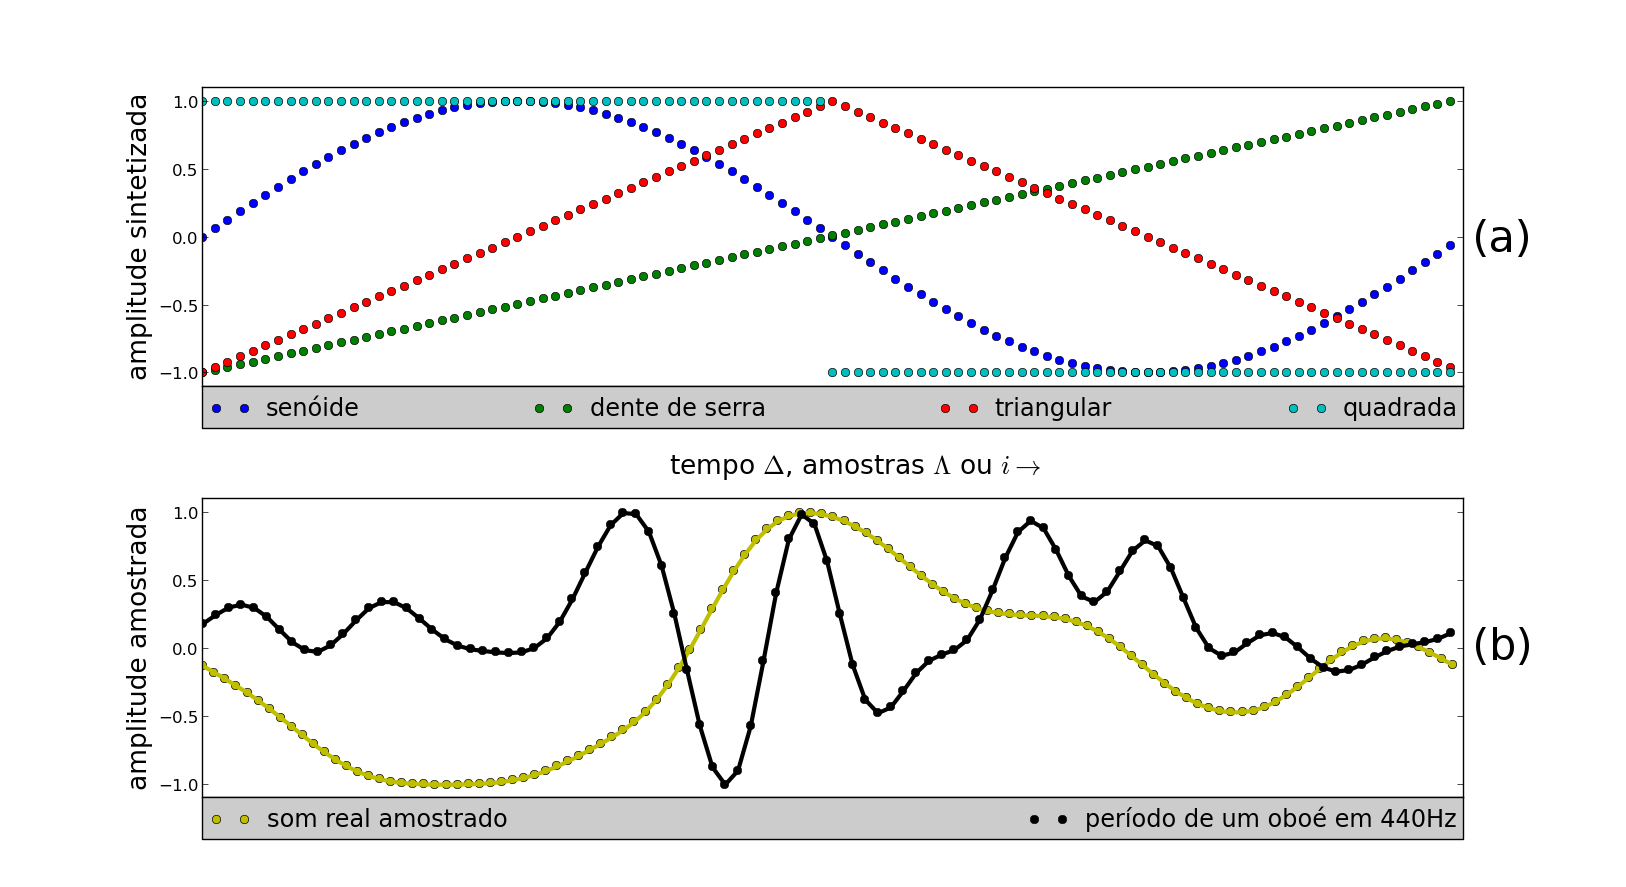
\includegraphics[width=\textwidth]{figuras/formasDeOnda6}
        \label{fig:formasDeOnda}
\end{figure}



A figura ~\ref{fig:formasDeOnda} apresenta
as formas de onda descritas nas equações ~\ref{senoide}, ~\ref{denteDeSerra}, ~\ref{triangular} e ~\ref{quadrada} para $\lambda_f=100$ (período
de $100$ amostras).
Se $t_a=44,1 kHz$, como no padrão PCM de Compact Disks, a onda possui frequência fundamental $f=\frac{f_a}{\lambda_f}=\frac{44100}{100} = 441 \; Herz $. Um lá\footnote{Um lá 4, logo acima do dó central, no segundo espaço do pentagrama na clave de sol comum.}, seja qual for a forma de onda dentre as artificiais apresentadas.

Estas formas de onda possuem usos especiais na música e seus espectros estão dispostos na figura ~\ref{fig:espectroDeOndas}. É importante notar as componentes isoladas e exatamente harmônicas dos espectros,
resultado de um período mantido fixo com exatidão. A senoide consiste de um nódulo único no espectro, frequência pura. A dente de serra é a única com a série harmônica completa (pares e ímpares). Já as ondas triangular e quadrada possuem as mesmas componentes espectrais, mas com decaimentos de $-12dB/oitava$ e $-6dB/oitava$.

\begin{figure}[h!]
    \centering
    \caption{Espectros das ondas sonoras musicais artificiais básicas}
        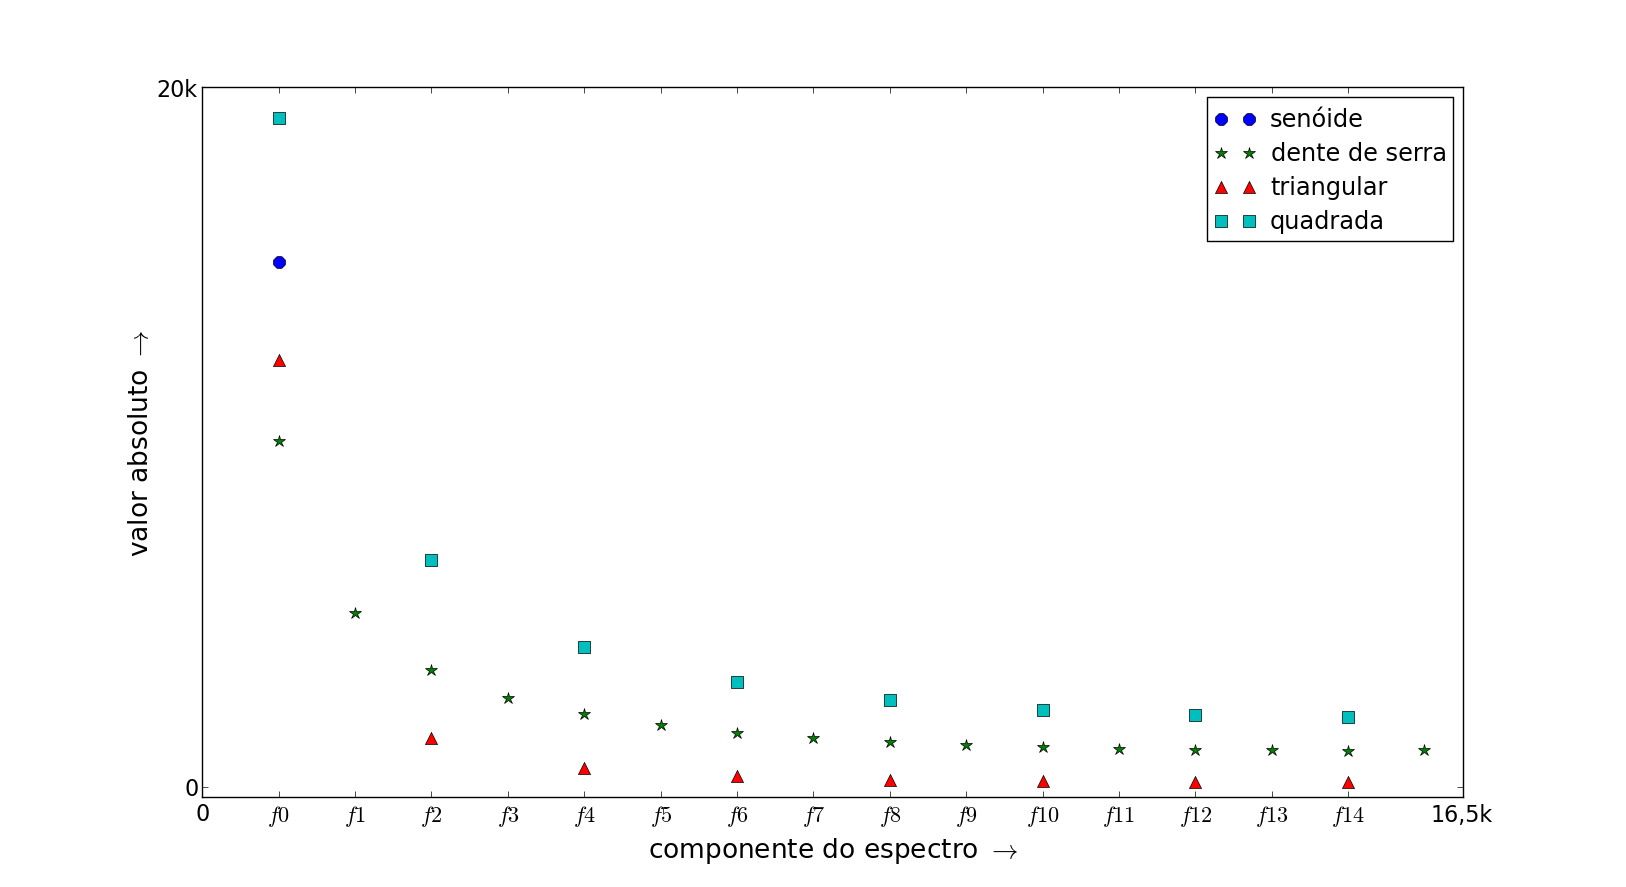
\includegraphics[width=\textwidth]{figuras/espectroDeOndas6}
        \label{fig:espectroDeOndas}
\end{figure}


O espectro harmônico é formado pelas frequências múltiplas da frequência fundamental $f_n=(n+1).f_0$.
Como nossa percepção segue uma progressão geométrica de frequências, o espectro possui notas diferentes da frequência fundamental. Além disso, o número de harmônicos será limitado pela frequência máxima $f_a/2$ (pelo Teorema de Nyquist). 

Musicalmente crucial aqui é internalizar que a presença de
energia\footnote{A energia total equivale à soma dos quadrados das amplitudes
(como as de pressao/voltagem no tempo), e.g. figura~\ref{fig:formasDeOnda}.
As componentes espectrais - e.g. figuras~\ref{fig:espectroDeOndas} e ~\ref{fig:espectroOboe} -
também podem ser elevadas ao quadrado para resultar em quantificação de energia e somam-se na energia total. As energias se equivalem pelo teorema de Parseval: $\frac{1}{\Lambda} . \sum_{k=0}^{\Lambda -1}c_k^2 = \sum_{i=0}^{\Lambda-1}t_i^2$.}
em uma componente de frequência $f_n$ na decomposição por fourier 
implica na presença de uma oscilação senoidal na constituição do som, puramente harmônica no som e naquela frequência $f_n$. Esta energia concentrada especificamente na frequência $f_n$ é separada
 pelo ouvido para adentrar em um nível cognitivo de processamento\footnote{Esta separação em frequência é realizada por diversas espécies através de mecanismos similares à cóclea humana~\cite{Roederer}.}.
  As componentes senoidais são geralmente as principais responsáveis pela qualidade chamada timbre e, caso não apresentem proporções harmônicas (relações de pequenos números), o som é percebido ruidoso, i.e. não são notas com frequência fundamental estabelecida unívocamente como um lá 4 ($440 Hz$) de nossos exemplos. Além disso, nossa noção de altura absoluta em um complexo sonoro é baseada na semelhança do espectro com a série harmônica~\cite{Roederer}.

No caso de uma forma de onda fixa (e de tamanho fixo), o espectro é sempre harmônico e estático. Fixada a frequência fundamental (inverso do comprimento da onda), cada forma de onda é composta de proporções específicas das componentes harmônicas e 
quanto maior a curvatura do trecho na forma de onda, maior a contribuição do trecho para a
concentração de energia nos harmônicos agudos.

Podemos ver isso claramente em sons reais. A onda rotulada como 'som real amostrado' na figura ~\ref{fig:formasDeOnda} é um período extraído de um som real relativamente comportado. Ele possuí $\lambda_f=114$ amostras\footnote{Caso também utilizado diretamente em $f_a=44,1kHz$, é um pouco mais grave que os $441 Hz$ das formas de onda artificiais $\frac{44100}{114}=385,84Hz$.}. A onda de oboé foi amostrada de um lá 4 também em $44,1kHz$.
O período escolhido para a amostragem é relativamente curto, com 98 amostras corresponde a 
uma frequência de $\frac{44100}{98}=450 Hz$. Pode-se perceber, através das curvaturas, o espectro rico em 
frequências agudas do oboé e o espectro mais grave do som real.

Note que, definindo $ R_i=\{ r_i \}_0^{\lambda_f-1}$ a sequência de amostras do som real da figura ~\ref{fig:formasDeOnda},
$R_i$ pode ser tomado como base para um som $T_i^f$ da seguinte forma: 

\begin{equation}\label{sampleandoFormaDeOnda}
     T^f_i=\{ t_i^f \}=\Bigl\{ r_{(i\,\%\lambda_{f})} \Bigr\}
\end{equation}

O som resultante possui o espectro momentâneo do som original. Por ser repetido de forma idêntica,
seu espectro é perfeitamente harmônico, sem os ruídos e variações típicas do fenômeno natural. Isso pode ser 
visto claramente na figura \ref{fig:espectroOboe} onde os espectros da nota original do oboé e de uma nota 
artificial - de mesma duração e cujas amostras consistem no mesmo período da figura ~\ref{fig:formasDeOnda} - estão dispostas juntamente. O espectro natural possui variações na frequência dos harmônicos, nas suas intensidades e uma quantidade de ruído. Já a nota cujo período foi amostrado possui espectro perfeitamente harmônico.



\begin{figure}[h!]
    \centering
    \caption{Espectros das ondas sonoras do oboé natural e de período amostrado}
        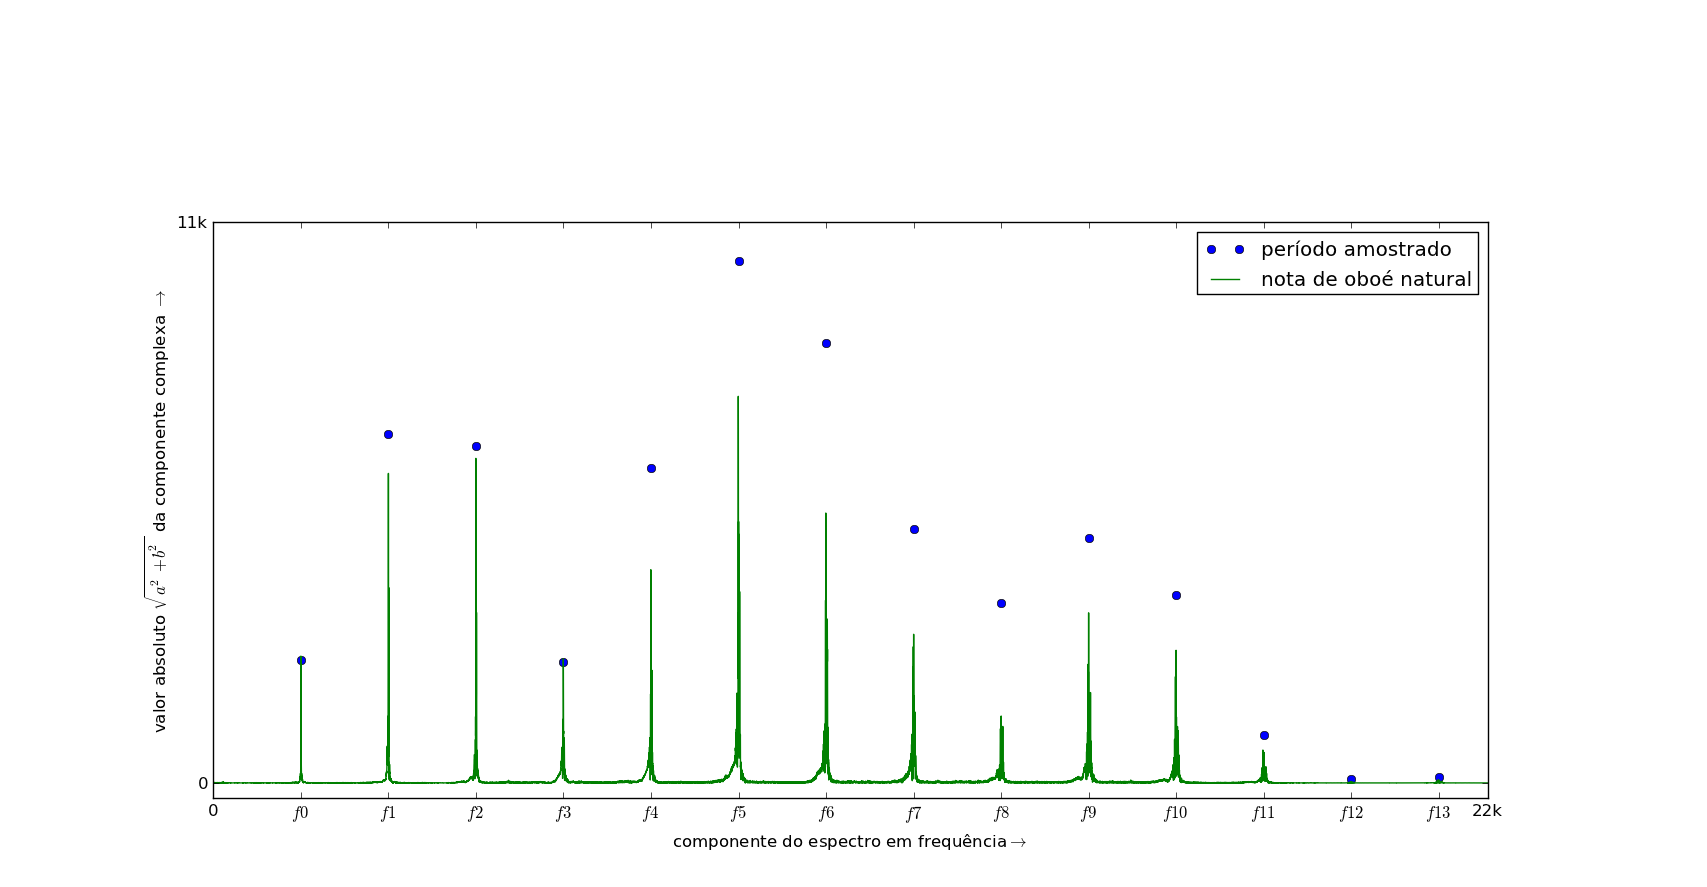
\includegraphics[width=\textwidth]{figuras/espectroOboeAmostradoNatural2}
        \label{fig:espectroOboe}
\end{figure}





\subsubsection{O espectro no som amostrado}
Além deste papel-chave na cognição (especialmente no timbre), a presença e comportamento destas componentes senoidais 
no som discretizado possui particularidades. Considere um sinal $T_i$ e sua decomposição de Fourier $\mathcal{F}\langle T_i\rangle=C_i=\{c_i\}_0^{\Lambda-1}$. Sabemos que a recomposição segue a conversão das componentes frequenciais em amostras temporais\footnote{Lembrando que o fator $\frac{1}{\Lambda}$ pode ser distribuído dentre a transformada e a reconstrução como preferir}:

 
\begin{equation}\label{recomposicaoFourier}
t_i = \frac{1}{\Lambda}\sum_{k=0}^{\Lambda-1}c_ke^{j \frac{2\pi k}{\Lambda} i } = \frac{1}{\Lambda}\sum_{k=0}^{\Lambda-1}(a_k+ j . b_k)\left[cos(w_k i) +j . sen(w_k i)\right]
\end{equation}

Onde $c_k = a_k + j . b_k$ pondera a amplitude e fase de cada frequência: $w_k=\frac{2\pi k}{\Lambda}$ em radianos ou $f_k=w_k\frac{f_a}{2\pi}=\frac{k.f_a}{\Lambda}$ em Herz (com atenção os respectivos limites em $\pi$ e em $\frac{f_a}{2}$). Nosso som possui amostras $t_i$ reais que resultam das contribuições de cada componente de frequência $w_k=\frac{2\pi k}{\Lambda}$ e cujo $c_k$ regula o módulo e a fase. A parte real da equação ~\ref{recomposicaoFourier} nos fornece a componente de forma mais clara:

\begin{equation}\label{moduloEfase}
\begin{split}
t_i& = \frac{1}{\Lambda}\sum_{k=0}^{\Lambda-1}\left[a_k cos(w_k i) -b_k sen(w_k i)\right] \\
   & = \frac{1}{\Lambda}\sum_{k=0}^{\Lambda-1}\sqrt{a_k^2 + b_k^2} \; cos\left[w_k i - tg^{-1}\left(\frac{b_k}{a_k}\right)\right]
\end{split}
\end{equation}

Podemos notar claramente pela equação ~\ref{moduloEfase} que o termo imaginário acrescenta uma fase à senoide real. Os termos imaginários $b_k$ da decomposição espectral por Fourier proporcionam a varredura de fase
 $[-\frac{\pi}{2},+\frac{\pi}{2}]$, basta observar o termo $tg^{-1}\left (\frac{b_k}{a_k}\right )$ que possui este contra-domínio. O sinal de $a_k$ especifica se estamos do lado direito ou esquerdo do circulo trigonométrico, completando a varredura completa de fase (os intervalos $[-\frac{\pi}{2},+\frac{\pi}{2}]$ e $[\frac{\pi}{2},\frac{3\pi}{2}]$ se justapõem em $2\pi$).


\begin{figure}[h!]
    \centering
    \caption{Oscilação de 2 amostras (frequência máxima em qualquer $f_a$)}
        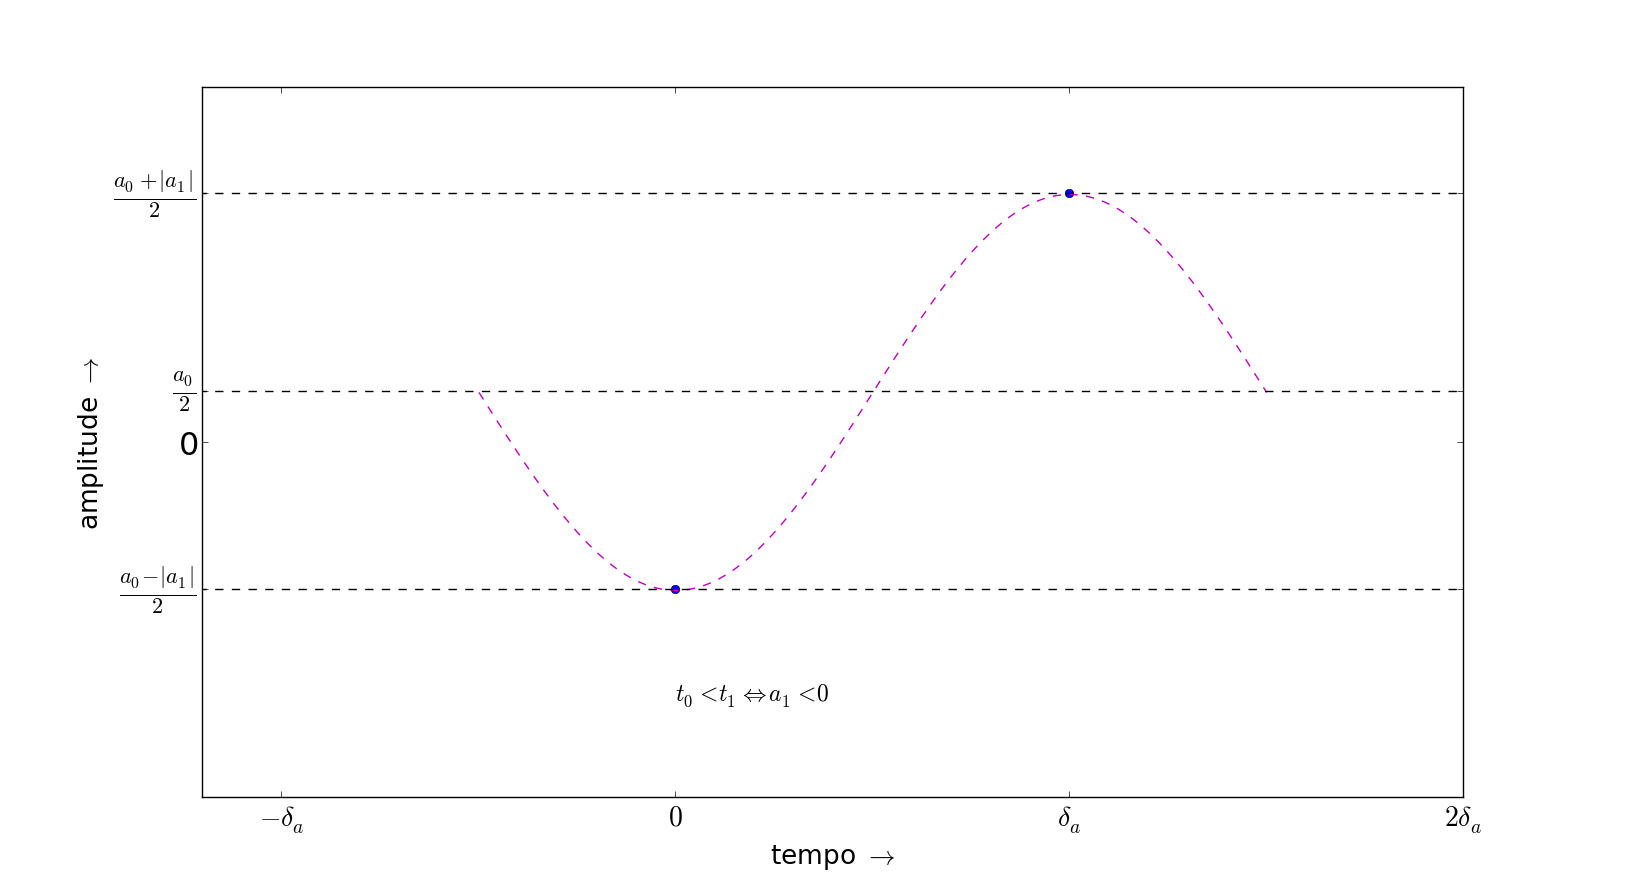
\includegraphics[width=\textwidth]{figuras/amostras2c__}
        \label{fig:amostras2}
\end{figure}

A figura ~\ref{fig:amostras2} exibe duas amostras e a componente espectral que contém. A decomposição de Fourier resulta neste caso em somente dois coeficientes $\{c_k=a_k-j.b_k\}_0^{\Lambda-1=1}$ relativos à frequências $\{f_k\}_0^1=\{w_k\frac{f_a}{2\pi}\}_0^1=\{k\frac{f_a}{\Lambda=2}\}_0^1=\{0,\frac{f_a}{2}=f_{\text{máx}}\}$
com energias $e_k=\frac{(c_k)^2}{\Lambda=2}$. O papel das amplitudes $a_k$ fica bem claro:
 $\frac{a_0}{2}$ é o deslocamento fixo\footnote{Chamado em vários contextos de \emph{bias} ou \emph{offset}.} e $\frac{a_1}{2}$ especifica a amplitude da oscilação em si, dada pela relação $f_k=k . \frac{f_a}{\Lambda=2}$.

Este caso é de especial importância pois o mínimo necessário para representar uma oscilação são 2 amostras e disso resulta a frequência de Nyquist $f_{\text{máx}}=\frac{f_a}{2}$. Esta é a frequência máxima presente em um som amostrado com $f_a$ amostras por segundo\footnote{Qualquer sinal amostrado possui esta característica, não somente o som digitalizado.}.

Vejamos o que acontece no caso de 3 amostras. Todas as sequências fixas $T_i$ de apenas 3 amostras também apresentam
somente 1 frequência, pois sua primeira harmônica usaria 1,5 amostras e ultrapassa o limite inferior de 2 amostras mínimas (a frequência da harmônica ultrapassaria a de Nyquist pois:  $\; \frac{2. f_a}{3} > \frac{f_a}{2} $). Se $\Lambda=3$, 
os coeficiêntes $\{c_k\}_0^{\Lambda-1=2}$ da decomposição por Fourier apresentam-se em 
3 componentes frequenciais. Uma delas é relativa à frequência zero ($c_0$), as outras duas ($c_1$ e $c_2$) contribuem de forma igual na reconstrução da senoide com $f=f_a/3$.

\begin{figure}[h!]
    \centering
    \caption{3 amostras apresentam uma única frequência}
        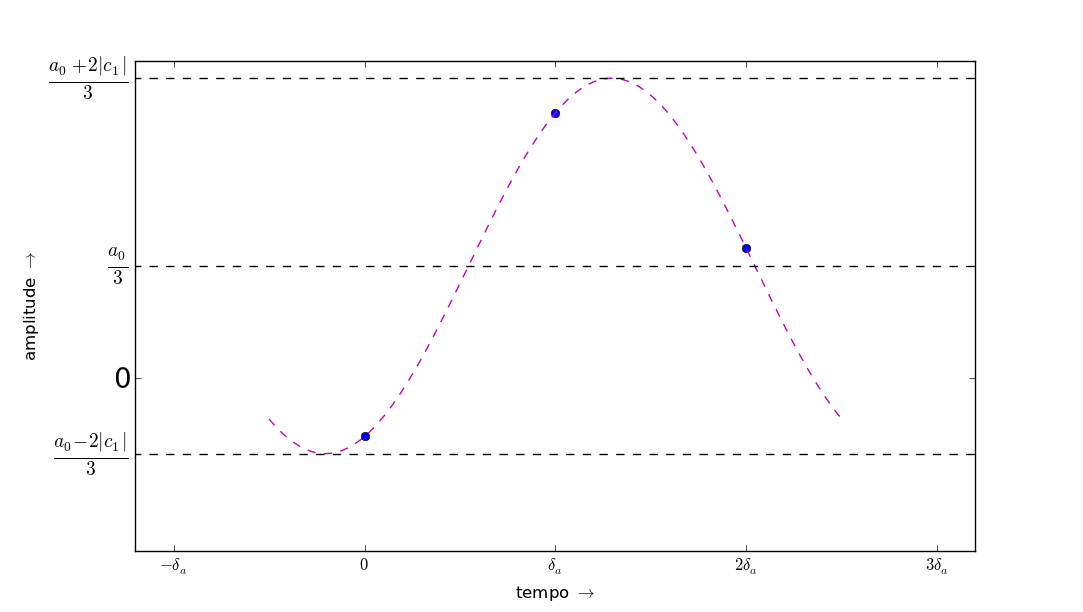
\includegraphics[width=\textwidth]{figuras/amostras3b}
        \label{fig:amostras3}
\end{figure}



Sempre que partimos de $\Lambda$ amostras reais $t_i$ resultamos em $\Lambda$ coeficientes complexos $c_k=a_k+j.b_k$. Os coeficientes $c_k$ se equivalem dois a dois\footnote{Parte real igual e imaginária com sinal trocado: $a_{k1}=a_{k2}$ e $b_{k1}=-b_{k2}$. Como consequência temos módulos iguais e fases com sinais opostos} correspondendo às frequências $f_k = k\frac{f_a}{\Lambda}, \; k \in \{0, ..., \left \lfloor \frac{\Lambda}{2} \right \rfloor \} $.
Quando $k> \frac{\Lambda}{2} $
a frequência $f_k$ é espelhada em $\frac{f_a}{2}$ da seguinte forma $f_k=\frac{f_a}{2} - (f_k-\frac{f_a}{2})=f_a-f_k=f_a - k\frac{f_a}{\Lambda}=(\Lambda-k)\frac{f_a}{\Lambda} \;\;\;\; \Rightarrow \;\;\;\; f_k\equiv f_{\Lambda-k} \; ,\;\; \forall \;\; k<\Lambda$. 

 
 O mesmo pode ser observado com 
 $w_k=f_k.\frac{2\pi}{f_a}$ e lembrando da periodicidade $2\pi$, que resulta em $w_k=-w_{\Lambda-k}$. Como o coseno é uma função par e a tangente inversa é impar, as componentes em $w_k$ e $w_{\Lambda-k}$ se somam na equação de reconstrução das amostras reais mostrada em ~\ref{recomposicaoFourier}.

  Dito de outra forma, em uma decomposição de $\Lambda$ amostras, as $\Lambda$ componentes frequenciais $\{c_i\}_0^{\Lambda-1}$ resultantes
   são equivalentes em pares.
   Excepcional excessão para $f_0$ e, no caso de $\Lambda$ ser par, de $f_{\Lambda/2}=f_{\text{máx}}=\frac{f_a}{2}$ , ambas as componentes são isoladas, i.e. não existe outra componente na frequência $f_0$ ou $f_{\Lambda/2}$ (se $\Lambda$ par) além dela mesma. 
Pois $f_{\Lambda/2}=f_{(\Lambda-\Lambda/2) = \Lambda/2}$ e $f_0=f_{(\Lambda-0)=\Lambda}=f_0$.

Além disso, estas duas frequências (a frequência zero e a frequência máxima) não são representadas com variação de fase e, portanto, são estritamente reais. Assim, podemos 
   concluir que o número $\tau$ de pares de coeficientes equivalentes é:

\begin{equation}\label{coefsPareados}
\tau = \frac{\Lambda - \Lambda \% 2}{2} +\Lambda \% 2 -1
\end{equation}

e resultam evidentes as equivalências ~\ref{equivalenciasFreqs}, ~\ref{equivalenciasModulos} e ~\ref{equivalenciasFases}:

\begin{equation}\label{equivalenciasFreqs}
f_{k}\equiv f_{\Lambda-k}\;, \;\; w_{k}=-w_{\Lambda-k}\;\;\;, \quad \;\; \forall \quad 1 \leq k \leq \tau  
\end{equation}

\begin{figure}[h!]
    \centering
    \caption{Componentes frequenciais em 4 amostras}
        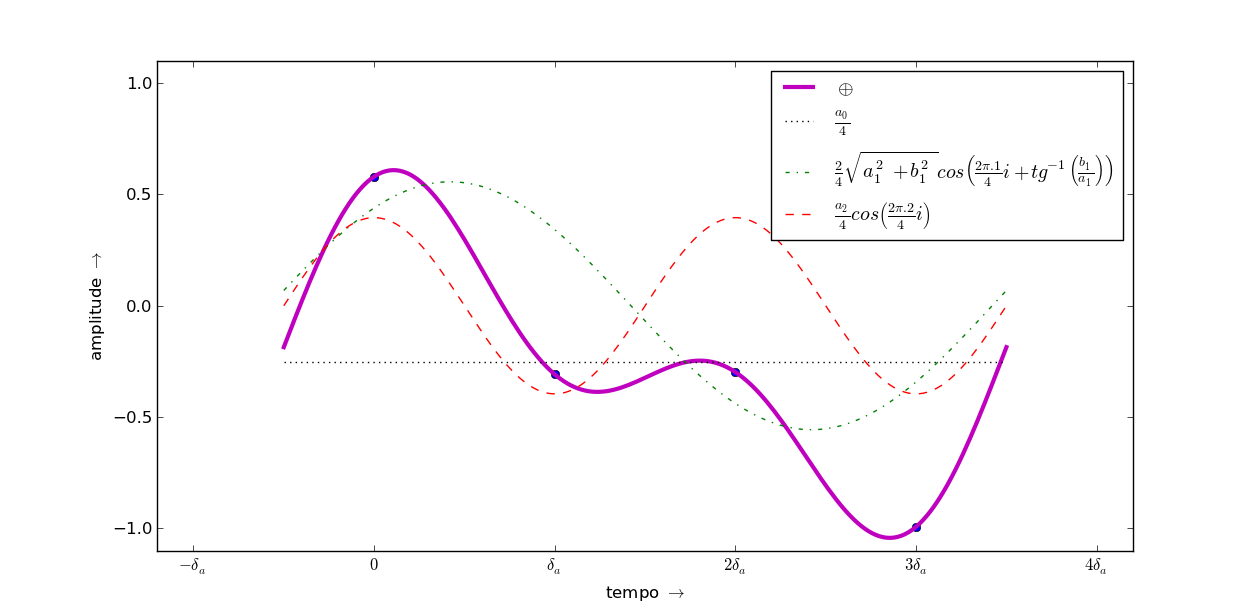
\includegraphics[width=\textwidth]{figuras/amostras4__}
        \label{fig:amostras4}
\end{figure}


Como $a_k = a_{\Lambda -k}\;\;$ e $\;\;b_k = - b_{\Lambda -k}$:

\begin{equation}\label{equivalenciasModulos}
\sqrt{a_k^2 + b_k^2} = \sqrt{a_{\Lambda - k}^2 + b_{\Lambda -k}^2} \;\;, \quad \;\; \forall \quad 1 \leq k \leq \tau  \\
\end{equation}

\begin{equation}\label{equivalenciasFases}
tg^{-1}\left(\frac{b_k}{a_k}\right)=-tg^{-1}\left(\frac{b_{\Lambda -k}}{a_{\Lambda - k}}\right)\;\;,\quad \;\; \forall \quad 1 \leq k \leq \tau
\end{equation}



Com $k \in \mathbb{N}$. A observação da equação de reconstrução para o sinal real ~\ref{moduloEfase} em conjunto com as equivalências dos módulos e fases ~\ref{equivalenciasModulos} e ~\ref{equivalenciasFases}, o número de coeficientes pareados \ref{coefsPareados} e equivalência de pares de frequências \ref{equivalenciasFreqs}
expõe o caso geral da combinação em fase das componentes em cada amostra $t_i$:

\begin{equation}
t_i = \frac{a_0}{\Lambda} + \frac{2}{\Lambda}\sum_{k=1}^{\tau}\sqrt{a_k^2 + b_k^2} \; cos\left[w_k i - tg^{-1}\left(\frac{b_k}{a_k}\right)\right]+ \frac{ a_{\Lambda/2}}{\Lambda}.(1-\Lambda\% 2)
\end{equation}

\begin{figure}[h!]
    \centering
    \caption{Formas de onda básicas em 4 amostras}
        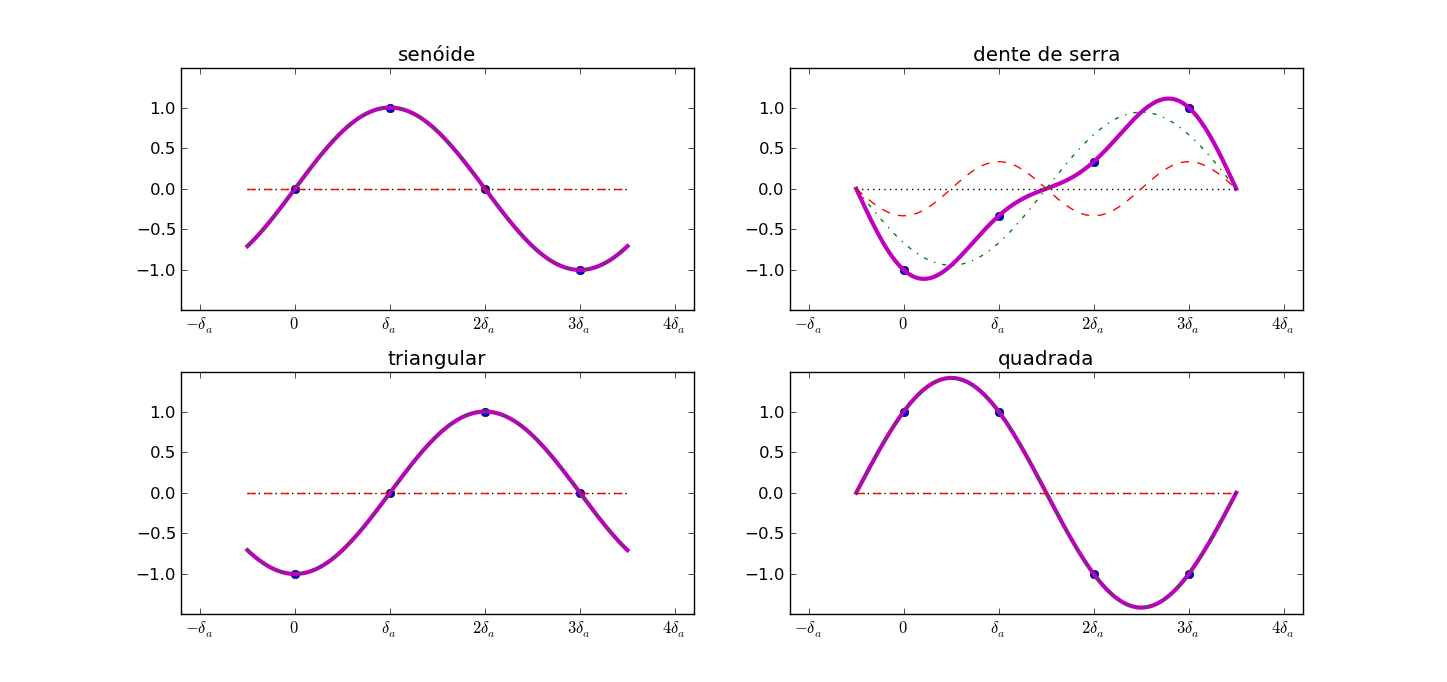
\includegraphics[width=\textwidth]{figuras/amostras4formas__}
        \label{fig:formas4}
\end{figure}


Assim, a exemplo da figura ~\ref{fig:amostras3}, a transformada de Fourier de 3 amostras possui 2 coeficientes frequenciais que possuem quantidades iguais de energia na mesma frequência.

Com 4 amostras, podemos representar 1 ou 2 frequências em proporções diferentes. A figura ~\ref{fig:amostras4} mostra uma 
forma de onda de 4 amostras e suas duas componentes. 
Note que as contribuições individuais se somam de fato na forma de onda 
original, e que as curvaturas maiores são fruto da frequência mais aguda
enquanto um deslocamento fixo da somatória das componentes é fruto
da componente na frequência zero.

A figura ~\ref{fig:formas4} explicita os harmônicos em 4 amostras nas formas de onda básicas das equações ~\ref{senoide}, ~\ref{denteDeSerra}, ~\ref{triangular} e ~\ref{quadrada} e figura ~\ref{fig:formasDeOnda}. Todas consistem em apenas 1 senoide, com excessão da dente de serra que possui os harmônicos pares.


A figura ~\ref{fig:amostras6} mostra uma decomposição senoidal para o caso de 6 amostras e a figura ~\ref{fig:formas6} decompõe as formas de onda básicas para o caso de 6 amostras.
 Note que neste caso de 6 amostras todas as ondas se diferenciam no espectro: as quadrada e triangular possuem as mesmas componentes, mas em proporções diferentes, já a dente de serra possui uma componente a mais.

\begin{figure}[h!]
    \centering
    \caption{Componentes frequenciais em 6 amostras}
        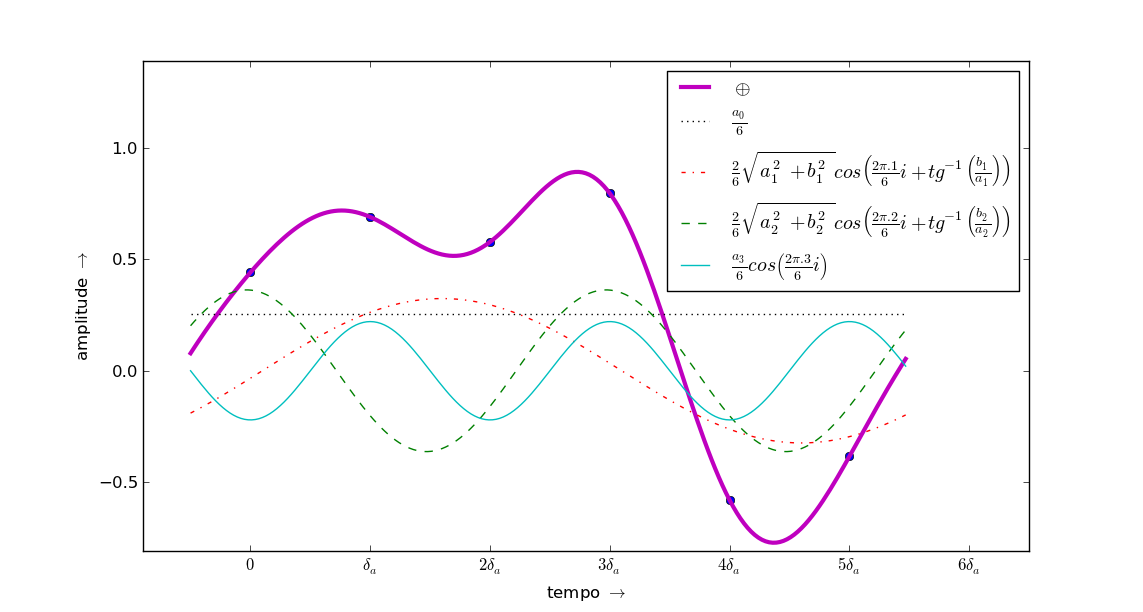
\includegraphics[width=\textwidth]{figuras/amostras6}
        \label{fig:amostras6}
\end{figure}

\begin{figure}[h!]
    \centering
    \caption{Formas de onda básicas em 6 amostras}
        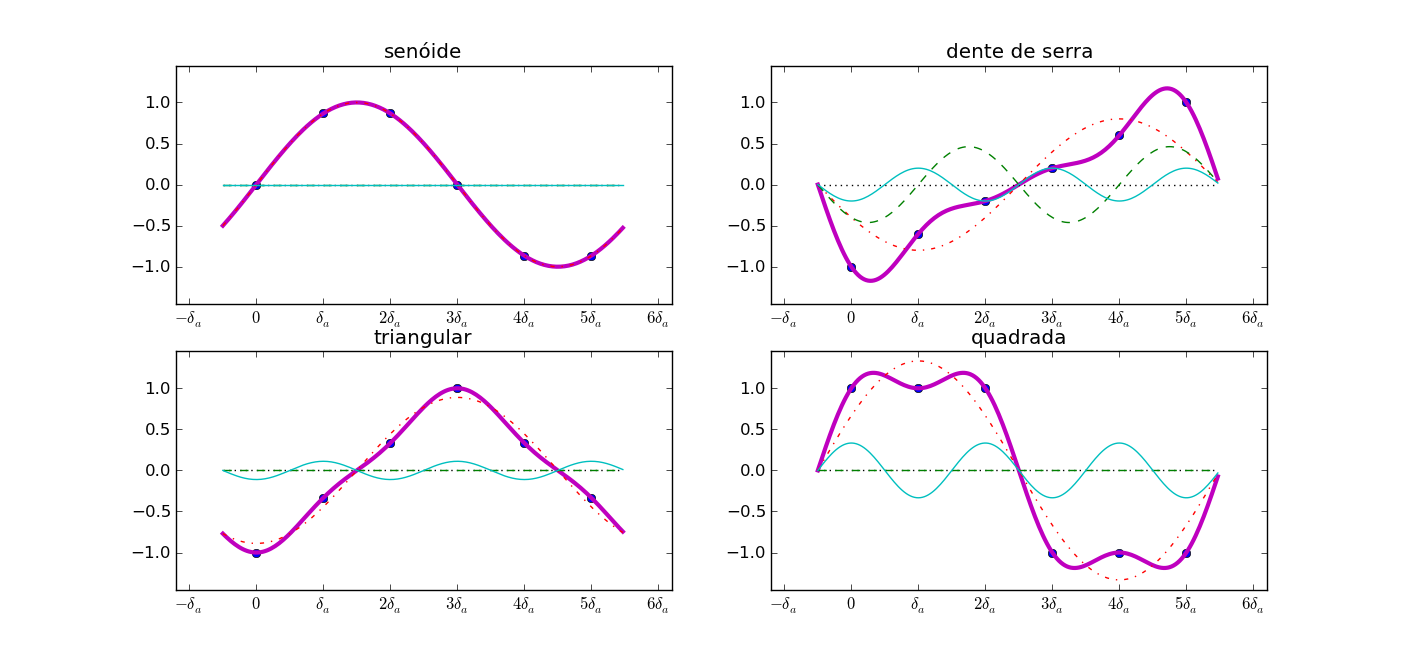
\includegraphics[width=\textwidth]{figuras/amostras6formas___}
        \label{fig:formas6}
\end{figure}

\subsubsection{Localização espacial}
Embora não seja uma das quatro qualidades básicas tradicionalmente elegidas para caracterizar uma nota musical,
a localização espacial é também importante para um som
pois este comumente é emitido por uma fonte localizada, como ocorre com um instrumento musical ou uma pessoa. Além disso, a espacialização é atributo bastante valorizado
 por audiófilos e pela indústria fonográfica~\cite{floEsp}.
Segundo a compreensão atual do fenômeno de percepção da localização espacial do som, nosso sistema nervoso utiliza
três informações: o atraso de chegada do som entre um ouvido e o outro, a diferença de intensidade do som direto em cada ouvido e a 
filtragem realizada pelo corpo, incluindo toráx, cabeça e orelhas~\cite{Roederer, hrtf, Heeger}.


\begin{figure}[h!]
    \centering
    \caption{Detecção de localização espacial de fonte sonora: DTI e DII}
        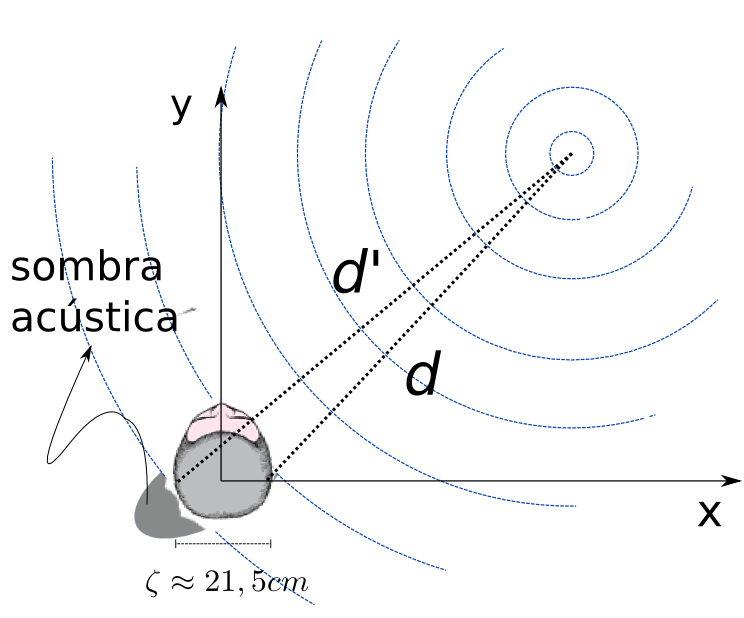
\includegraphics[width=.5\textwidth]{figuras/espacializacao___}
        \label{fig:spac}
\end{figure}



	Se consideradas somente as incidências diretas em cada ouvido, podemos dispor as diferenças de tempo e intensidade em equações simples. Dada a distância entre os ouvidos $\zeta\approx 21,5cm$,
um objeto localizado em $(x,y)$ conforme a figura~\ref{fig:spac}
está distante de cada ouvido:

\begin{equation}
\begin{split}
d & =\sqrt{\left (x-\frac{\zeta}{2} \right )^2+y^2} \\
d' & =\sqrt{\left (x+\frac{\zeta}{2} \right )^2 + y^2}
\end{split}
\end{equation}


e cálculos imediatos nos levam à DTI (Diferença de Tempo Interaural)\footnote{Constata-se que $\zeta \approx 21,5cm$ para um humano adulto.}:

\begin{equation}
DTI=\frac{d'-d}{v_{som\;no\;ar}\approx 343,2 }\quad \text{segundos}
\end{equation}

e à DII (Diferença de Intensidade Interaural):
\begin{equation}
DII=20\log_{10}\left (\frac{d'}{d}\right) \quad dBs
\end{equation}

Convertendo para amplitude temos $DII_a=\frac{d'}{d}$. A $DII_a$ pode
ser utilizada como constante multiplicativa do canal direito de um sinal sonoro estéreo ($\{t_i\}_0^{\Lambda -1}=\{DII_a . t_i'\}_0^{\Lambda -1}$). Pode-se utilizar a DII junto à DTI como adiantamento no tempo do canal direito com relação ao esquerdo, vínculo crucial para a percepção de localidade em sons graves e em sonoridades percussivas~\cite{Heeger}.
Considerando $\Lambda_{DTI}=\lfloor DTI . f_a \rfloor $, podemos escrever:

\begin{equation}
\begin{split}
\Lambda_{DTI} & = \left \lfloor \frac{d'-d}{343,2}  f_a \right \rfloor \\
DII_a & = \frac{d'}{d} \\
\{t_{(i+\Lambda_{DTI})}\}_{\Lambda_{DTI}}^{\Lambda+\Lambda_{DTI}-1} & =\{DII_a . t_i'\}_0^{\Lambda-1} \\
\{t_i\}_0^{\Lambda_{DTI}-1} & = 0
\end{split}
\end{equation}

Com $t_i$ o canal direito e $t_i'$ o canal esquerdo. Caso $\Lambda_{DTI} < 0 $, basta trocar $t_i$ por $t_i'$  e utilizar $\Lambda_{DTI}'= | \Lambda_{DTI} | $.

Embora consideravelmente simples até aqui, a localização espacial depende drasticamente de outras pistas. De forma canonica, resolvemos pelas
DTI e DII somente o ângulo horizontal (azimutal) $\theta$ dado por:

\begin{equation}
\theta=\tan^{-1}\left ( \frac{y}{ x }  \right )
\end{equation}

Mesmo assim, há dificuldades quando $\theta$ incinde sobre o chamado "cone de confusão" em que um mesmo par de especificações DTI, DII resultam de vários dos pontos 
do cone. Nestes pontos, a inferência do ângulo azimutal depende especialmente da filtragem atenuante nos agudos, pois a cabeça interfere um tanto mais nas ondas mecânicas agudas do que nas graves~\cite{Heeger,hrtf}. 

A figura~\ref{fig:spac} mostra esta sombra acústica do crânio, importante para a percepção do ângulo azimutal da fonte no cone de confusão. O cone em si não foi disposto na figura pois não é exatamente um cone e suas dimensões precisas não são especificadas na literatura~\cite{confCone}, mas pode ser entendido como um cone com o ápice no meio da cabeca e saindo por cada uma das orelhas.

Já a localização completa, incluindo distância e elevação da fonte sonora, é dada pela função de transferência de cabeça (HRTF - do inglês \emph{Head Related Transfer Function}~\cite{hrtf}. Exitem bases abertas e conhecidas de HRTF como \emph{CIPIC}~\cite{CIPIC} e podemos aplicar estas funções de transferência em um som por convolução (veja equação~\ref{eq:conv}). Estas funções de transferência mudam de acordo com o corpo do indivíduo e existem diversas técnicas para resultar em funções de transferência que sejam utilizáveis de forma mais universal~\cite{lazaSPA}. 


\subsubsection{A nota básica}\label{notaBasica}

Escolhamos $f$ tal que $f$ divida $f_a$  
 \footnote{Como apontado anteriormente, esta escolha facilita as demonstrações.
Transporemos esta limitação na próxima sessão.}. 
Uma sequência $T_i$ de amostras sonoras separadas por $\delta_a=1/f_a$ descreve uma nota musical de frequência $f$ Herz e duração $\Delta$ segundos se, e somente se, possuir a periodicidade $\lambda_f=f_a/f$
 e tamanho $\Lambda=\lfloor f_a . \Delta \rfloor $:

\begin{equation}
T_i^{f,\; \Delta}=\{t_{i \, \% \lambda_f} \}_0^{\Lambda-1}= \left \{t_{i \; \% \left( \frac{f_a}{f} \right) } \right \}_0^{\Lambda-1}
\end{equation}

Note que a nota por si só não especifica um timbre. Mesmo assim, faz-se necessária a escolha de uma forma de onda para que as amostras $t_i$ tenham um valor estabelecido individualmente. Um único período dentre as ondas básicas pode ser utilizado para a especificação da nota da seguinte forma:

seja $f$ a frequência da nota e escolhamos $f$ tal que $f$ divida $f_a$ (transporemos esta limitação na sessão seguinte). Assim, o inteiro $\lambda_f=\frac{f_a}{f}$ é o número de amostras do período. Temos que $L_i^{f,\, \delta_f} $ é
a sequência que descreve um período da onda $L_i^f \in \{S_i^f,Q_i^f,T_i^f,D_i^f,R_i^f \}$ de duração 
$\delta_f=1/f$ (ver equações ~\ref{senoide}, ~\ref{denteDeSerra}, ~\ref{triangular} e ~\ref{quadrada}; $R_i^f$ 
é uma onda real amostrada):

\begin{equation}\label{periodoUnico}
L_i^{f , \delta_f } = \{ l_i^f \}_0^{\delta_f . f_a -1}=\{ l_i^f \}_0^{\lambda_f-1}
\end{equation}

Então a sequência $T_i$ consistirá em uma nota de duração $\Delta$ e frequência $f$ se:

\begin{equation}
T_i^{f,\; \Delta}=\{t_i^f\}_0^{\lfloor f_a . \Delta \rfloor -1}=\left \{ l^f_{i\,\%\left(\frac{f_a}{f}\right)} \right \}_0^{\Lambda-1}
\end{equation}


\subsubsection{Usos musicais}


Em posse da nota básica, podemos montar estruturas musicais com
sequências destas partículas. Caso somemos $N$ sequências ($T_{k,i}=\{t_{k,i}\}, \;\; k \in 0...N-1$) de mesmo tamanho, seus conteúdos espectrais serão sobrepostos e a isso damos o nome de mixagem:

\begin{equation}\label{eq:mixagem}
\{t_i\}=\left \{ \sum_{k=0}^{N-1}t_{k,i} \right \}
\end{equation}

\begin{figure}[h!]
    \centering
    \caption{Mixagem de três sequências sonoras}
        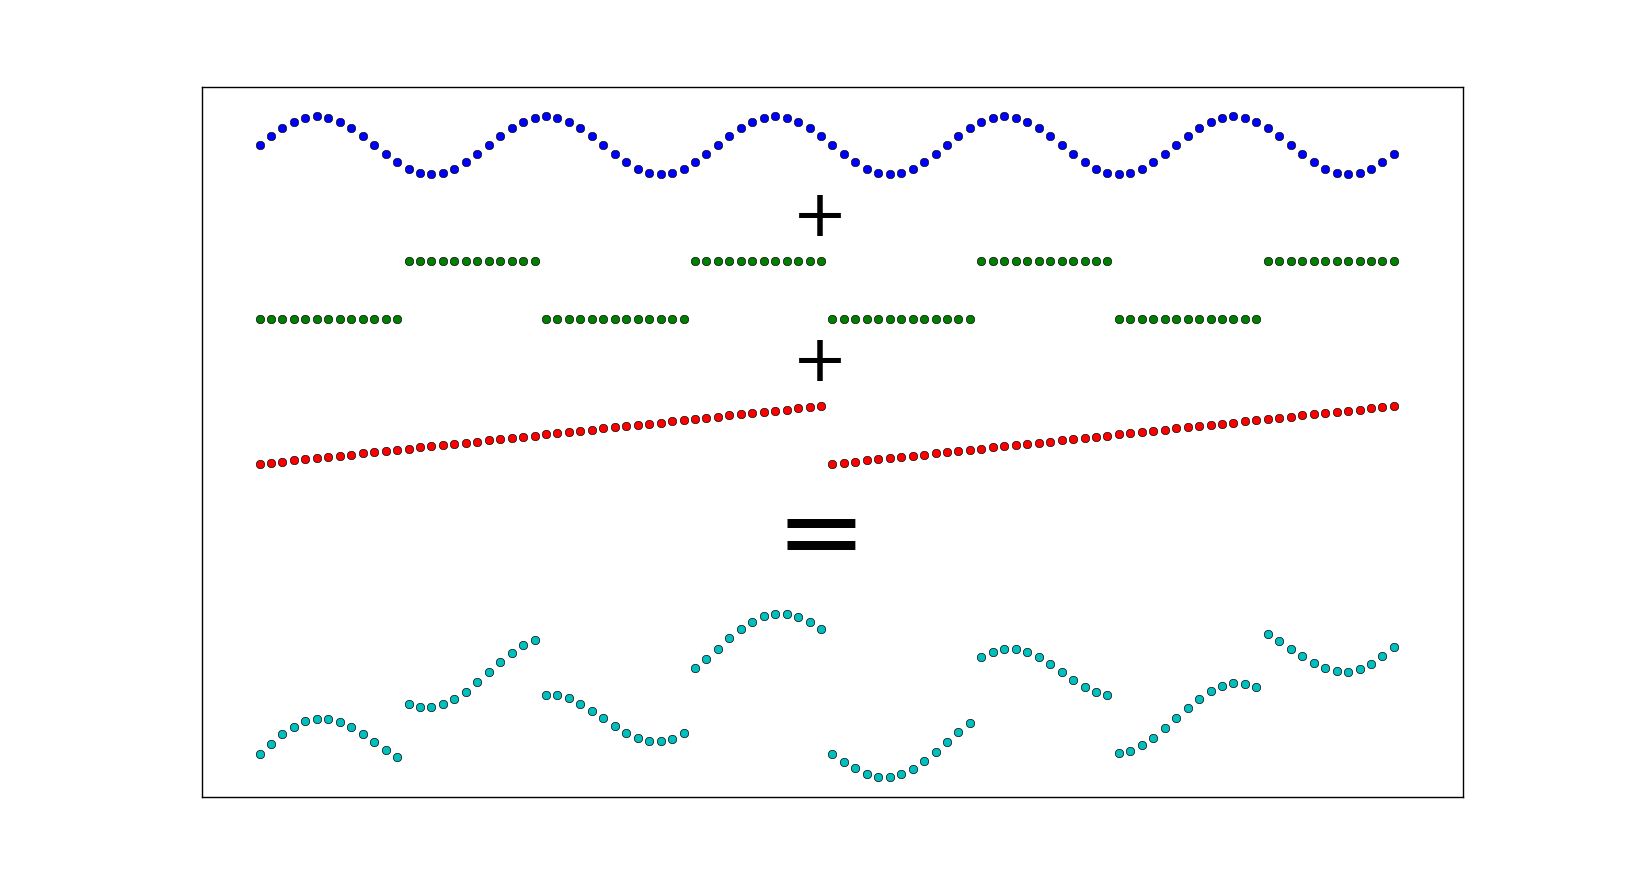
\includegraphics[width=\textwidth]{figuras/mixagem}
        \label{fig:mixagem}
\end{figure}


Ilustramos na figura~\ref{fig:mixagem} este processo de superposição de ondas sonoras discretizadas\footnote{A figura dispõe 100 amostras, de onde podemos concluir que, se $f_a=44,1kHz$, as frequências da dente de serra, da onda quadrada e da senoide são,
respectivamente, $\frac{f_a}{50}=882Hz$, $\frac{f_a}{25}=1764Hz$ e $\frac{f_a}{20}=2205Hz$. A duração do trecho é bastante curto $\frac{f_a=44,1kHz}{100} \approx 2 \text{ milisegundos}$.}.
 As notas mixadas são em grande parte separadas pelo ouvido por leis físicas de ressonância e pelo sistema nervoso~\cite{Roederer}.

Pode-se completar com zeros para somar sequências de tamanhos diferentes. O resultado da mixagem de notas musicais é a harmonia musical, cujos intervalos entre as frequências e os acordes de notas simultâneas regem aspectos subjetivos e abstratos da música e sua apreciação~\cite{Harmonia}. 

As sequências podem também ser concatenadas no tempo. Caso as sequências $\{t_{k,i}\}_0^{\Lambda_k-1}$ de tamanhos $\Lambda_k$  representem $k$ notas musicais, sua concatenação em uma única sequência $T_i$ resultará em uma sequência musical simples ou melodia:

\begin{equation}
\{t_i\}_0^{\sum\Delta_k-1}=\{t_{l,i}\}_0^{\sum\Delta_k-1}, \;\; l\text{ menor inteiro } : \quad \Lambda_l > i -\sum_{j=0}^{l-1}\Lambda_j
\end{equation}

Este mecanismo é demonstrado de forma ilustrativa na figura~\ref{fig:concatenacao} com as mesmas sequências utilizadas na figura ~\ref{fig:mixagem}.
 As sequências são curtas para as taxas de amostragem usuais (cerca de $7$ milisegundos ao total se $f_a=44,1kHz$), mas pode-se observar de forma explícita a concatenação de sequências sonoras e o exemplo é real (cada nota tem a duração maior que $100ms$ se $f_a<1kHz$).

\begin{figure}[h!]
    \centering
    \caption{Concatenação de três sequências sonoras}
        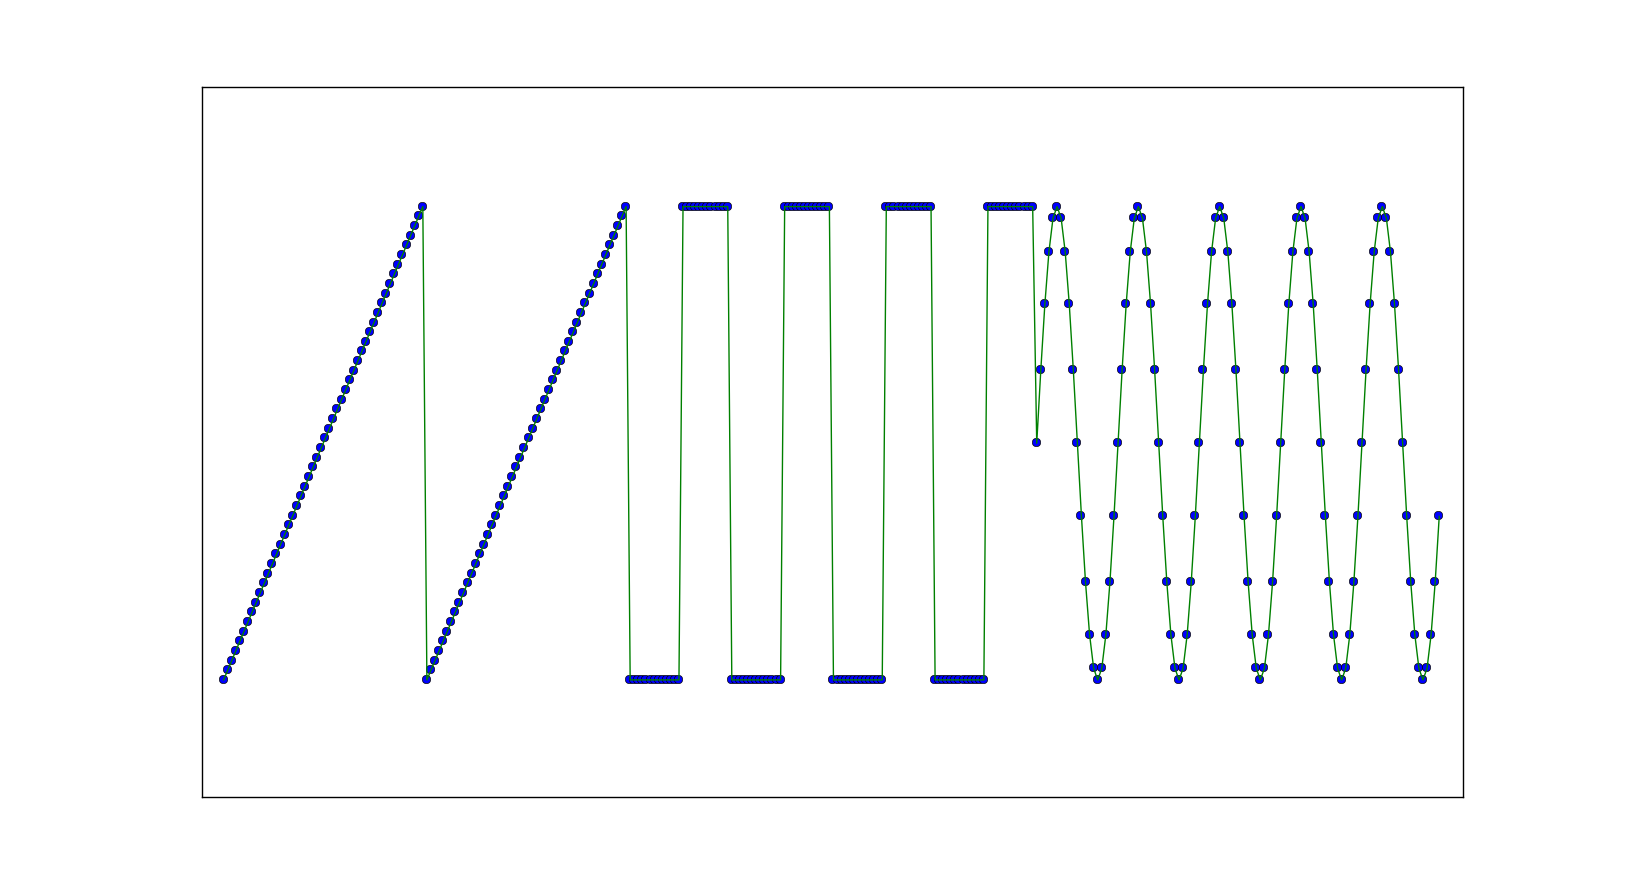
\includegraphics[width=\textwidth]{figuras/concatenacao}
        \label{fig:concatenacao}
\end{figure}

A montagem musical \emph{reduced-fi} demonstra de forma isolada este uso de justaposição temporal das notas, resultando em uma peça homofônica. O princípio vertical está demonstrado nos \emph{quadros sonoros}, sons estáticos com espectros peculiares. Ambas as peças estão em código Python no APÊNDICE~\ref{cap:codigoPecas} e podem ser escutadas e vizualizadas nos links~\cite{reduced-fi} e~\cite{quadros}.

Com isso estabelecemos nossa nota musical básica no som digital. Trabalharemos a seguir estas unidades, a evolução temporal de seus conteúdos e desenvolveremos as notas musicais com parâmetros que evoluem no tempo, como glissandos e envoltórias. 
A filtragem de componentes e os ruídos finalizam sobre a constituição da nota musical como unidade isolada. A estruturação musical destas notas é então abordada do ponto de vista das estruturas fora do tempo (como as escalas), trajetórias cíclicas ou que convirjam ou divirjam.

\clearpage

\subsection{Variações na nota musical básica}

Nossa nota musical digital básica está bem definida com os parâmetros:
duração, altura, intensidade (volume) e timbre. Esta é uma modelagem
útil e paradigmática, mas não esgota o que entendemos por
uma nota musical.

Em primeiro lugar, as características da nota se modificam no decorrer
da própria nota, i.e. em uma nota real os parâmetros
não são absolutamente fixos~\cite{Chowning}. Por exemplo, em uma nota de piano
de 3 segundos, a intensidade tem início abrupto e decaimento progressivo
além de variações do espectro instantâneo, com harmônicos que
decaem antes dos outros e alguns que aparecem com o tempo.
Estas variações não são obrigatórias e sim orientações da
síntese sonora para usos musicais pois é como os sons
se apresentam na natureza\footnote{A regra de ouro
aqui é: para que um som isolado disperte interesse
por si só, faça como que tenha variações internas~\cite{Roederer}.}. 

Explorar todas as formas pelas quais estas variações ocorrem está fora
do escopo de qualquer trabalho dada a considerável sensibilidade do ouvido humano
e a complexidade da nossa cognição sonora. Desta forma, apontaremos
recursos primários para estas variações das características na nossa nota
básica.

Iniciaremos com uma técnica que não resulta propriamente
em variações internas da nota, mas simplificará esta exposição
sem restringir o escopo, além de ser um notável recurso de otimização
computacional.



\subsubsection{Tabela de Busca}

Mais conhecido pelo termo em inglês, a \emph{Lookup Table} (ou simplesmente
LUT), é um procedimento simples que consiste em criar uma tabela
de referência e coletar as amostras desta tabela segundo a 
necessidade\footnote{Em contraposição ao cálculo das amostras individuais
de forma analítica.}. Em nosso caso, usaremos tabelas de busca para os
sons criados, as notas. Assim, estas tabelas são unidimensionais e com
valores reais. Além disso, a tabela consiste nas amostras
de um período de onda, que usamos para sintetizar períodos
de tamanhos diferentes, resultando em frequências diferentes.

O procedimento de busca em tabelas é visto geralmente como um
artifício de otimização. Na música seu uso transcende este
primeiro, facilitando as operações e permitindo que um único
período de onda possa ser usado para sintetizar sons em toda a banda
de frequências audíveis, qualquer que seja a forma de onda amostrada.

Descrevemos esta busca. Seja $\widetilde{\Lambda}$ o tamanho 
da tabela e $\widetilde{L_i} = \{ \widetilde{l}_i \}_0^{\widetilde{\Lambda} -1}$ a tabela de elementos $\widetilde{l_i}$ de um
período de onda qualquer (veja equação ~\ref{periodoUnico}). Uma sequência
$T_i^{f,\,\Delta}$ com amostras de um som de frequência $f$ e duração $\Delta$
pode ser feita a partir de $\widetilde{L_i}$ da seguinte forma:

\begin{equation}
T_i^{f,\,\Delta}=\{t_i^f\}_0^{\lfloor f_a . \Delta \rfloor -1} = \{ \widetilde{l}_{\gamma_i \% \widetilde{\Lambda} } \}_{0}^{\Lambda-1}\; , \quad \text{onde} \;\; \gamma_i = \left \lfloor i . f \frac{ \widetilde{\Lambda}}{f_a} \right \rfloor  
\end{equation}

Ou seja, dada a tabela de busca, basta termos a sequência de índices corretos
para sintetizar o som em qualquer frequência. Para o cálculo do inteiro $\gamma_i$, convencionamos
atribuir a ele o maior inteiro menor que $i.f\frac{\widetilde{\Lambda}}{f_a}$.
Esta aproximação introduz um ruído, mas conseguimos que este ruído seja desprezível
mesmo se o tomarmos como o maior inteiro acima da multiplicação
ou se arredondarmos por outros métodos. Além disso, para fins de síntese, em $f_a=44,1 kHz$
 o padrão é usar $\widetilde{\Lambda} = 1024$ amostras, pois já não gera ruído
 relevante no espectro audível~\cite{Geiger}.

 A expressão que define a variável $\gamma_i$ pode ser facilmente compreendida da
 seguinte forma: a variável $i$ é acrescida de $f_a$ em $1$ segundo (pela
 definição de $f_a$ e $i$, pois temos $f_a$ amostras $t_i$ em $1$ segundo). Caso a dividamos por $f_a$, teremos $\frac{i}{f_a}$,
fração esta que é acrescida de $1$ a cada $1$ segundo. Multiplicado pelo comprimento da
 tabela $\widetilde{\Lambda}$, teremos $i \frac{\widetilde{\Lambda}}{f_a}$
 que resulta na varredura completa da tabela $\widetilde{L_i}$ em 
 1 segundo com o acréscimo de $\widetilde{\Lambda}$ em $1$ segundo. Por fim,
 se multiplicarmos pela frequência $f$ que queremos, teremos $i . f \frac{\widetilde{\Lambda}}{f_a}$
 que resulta em $f$ varreduras completas da tabela $\widetilde{L_i}$ em $1$ segundo, i.e. a sequência
 resultante apresenta a frequência fundamental $f$.

Importantes considerações: $f$ é qualquer, só há limitantes nas frequências
graves quando o tamanho da tabela $\widetilde{\Lambda}$ não é suficientemente grande para a taxa de amostragem
$f_a$. O procedimento de busca em tabela
é computacionalmente bastante barato, substituindo cálculos por buscas simples (por isso geralmente
é entendido como um processo de otimização). Salvo quando assinalado,
no texto que segue usaremos este procedimento para todos os casos cabíveis pois
simplifica diversas rotinas e é computacionalmente coerente. Para um uso clássico das LUTs na síntese sonora musical, recomendamos procurar pela chamada \emph{Wavetable Synthesis} que consiste em várias LUTs utilizadas em conjunto através da mixagem para gerar uma nota musical quasi-periódica~\cite{Cook,Wavetable}.


\subsubsection{Variações incrementais de frequência e intensidade}

Segundo revela a lei de Weber e Fechner, nossa percepção tem uma relação logarítmica com
o estímulo que a causa~\cite{Weber-Fechner}. Mesmo assim, dado o uso, explicitaremos também a variação
linear e começaremos descrevendo esta por razões didáticas.

Em uma nota de duração $\Delta = \frac{\Lambda}{f_a}$, a frequência $f=f_i$ varia de $f_0$ até $f_{\Lambda -1}$
linearmente. Podemos então escrever que:

\begin{equation}\label{freqLinear}
f_i=f_0 + (f_{\Lambda-1}-f_0)\frac{i}{\Lambda-1} \quad ,\quad \quad i \;\in\; \mathbb{N}, \quad i \;\in\; [0,\Lambda-1]
\end{equation}

\begin{equation}\label{indiceLinear}
\Delta_{\gamma_i}=f_i\frac{\widetilde{\Lambda}}{f_a} \quad \Rightarrow \quad \gamma_i=\left \lfloor \sum_{j=0}^{i} f_i\frac{\widetilde{\Lambda}}{f_a} \right \rfloor   =\left \lfloor \sum_{j=0}^{i}  \frac{\widetilde{\Lambda}}{f_a} \left [f_0 + (f_{\Lambda-1}-f_0)\frac{i}{\Lambda-1} \right ] \right \rfloor 
\end{equation}

\begin{equation}\label{serieAmostralLin}
\{t_i^{\;\overline{f_0,\, f_{\Lambda-1}}}\}_0^{\Lambda-1}=\{\widetilde{l}_{\gamma_i \% \widetilde{\Lambda}}\}_0^{\Lambda-1}
\end{equation}

Onde $\Delta_{\gamma_i}=f_i\frac{\widetilde{\Lambda}}{f_a}$ é o incremento da LUT entre duas amostras dada a frequência do som na primeira amostra.

Desta forma, podemos calcular os elementos $t_i^{\;\overline{f_0,f_{\Lambda-1}}}$
com base no período $\{\widetilde{l}_i\}_0^{\Lambda-1}$.

As equações \ref{freqLinear}, \ref{indiceLinear} e \ref{serieAmostralLin} são relativas à progressão linear
da frequência. Como assinalado, nossa percepção segue a progressão logarítmica:
uma progressão de frequência
\emph{percebida} como linear segue uma progressão exponencial\footnote{Ou,
dito ainda de outra forma, uma progressão geométrica da frequência
é percebido como uma progressão aritmética de alturas.}.

Fazendo a varredura com $i$
de $0$ até $\Lambda-1$, podemos dizer que: $f_i=f_0 . 2^{\frac{i}{\Lambda-1} n_8}$ onde 
$n_8=\log_2\frac{f_{\Lambda-1}}{f_0}$ é o número de oitavas entre $f_0$ e $f_{\Lambda-1}$.
De forma que $f_i=f_0 . 2^{\frac{i}{\Lambda-1}\log_2\frac{f_{\Lambda-1}}{f_0}}=
f_0 . 2^{\log_2\left ( \frac{f_{\Lambda-1}}{f_0} \right )^{\frac{i}{\Lambda-1}}}=
f_0 \left ( \frac{f_{\Lambda-1}}{f_0} \right ) ^{\frac{i}{\Lambda -1}}$. Portanto,
nossas equações de referência para a síntese de transições de frequência tidas como
lineares pelo ouvido são:

\begin{equation}
f_i=f_0 \left ( \frac{f_{\Lambda-1}}{f_0} \right ) ^{\frac{i}{\Lambda -1}}
\end{equation}

\begin{equation}\label{indiceExponencial}
\Delta_{\gamma_i}=f_i\frac{\widetilde{\Lambda}}{f_a} \quad \Rightarrow \quad \gamma_i=\left \lfloor \sum_{j=0}^{i} f_i\frac{\widetilde{\Lambda}}{f_a} \right \rfloor   =\left \lfloor \sum_{j=0}^{i} f_0 \frac{\widetilde{\Lambda}}{f_a} \left ( \frac{f_{\Lambda-1}}{f_0} \right ) ^{\frac{i}{\Lambda -1}} \right \rfloor
\end{equation}

\begin{equation}\label{serieAmostralLog}
\{t_i^{\;\overline{f_0,\,f_{\Lambda-1}}}\}_0^{\Lambda-1}=\{\widetilde{l}_{\gamma_i \% \widetilde{\Lambda}}\}_0^{\Lambda-1}
\end{equation}

Onde usamos a equação \ref{indiceExponencial} para calcular a sequência $\{\gamma_i\}_0^{\Lambda-1}$ de índices para para
serem buscados na nossa tabela que contém um único período da forma de onda representado em uma sequência de $\widetilde{\Lambda}$
pontos igualmente espaçados (amostras).
Isso é explicitado na equação ~\ref{serieAmostralLog}, onde estabelecemos a relação
 $t_i^{\;\overline{f_0,f_{\Lambda-1}}}=\widetilde{l}_{\gamma_i \% \widetilde{\Lambda}}$.
Note que a equação \ref{serieAmostralLog} se mantém (permanece idêntica à equação \ref{serieAmostralLin}).

O termo $\frac{i}{\Lambda-1}$ varre o intervalo $[0,1]$ e podemos elevá-lo a uma potência
para que o início da transição seja mais suave ou mais abrupto (compensado pelo final
da transição). Este procedimento é mais comum para o caso de variações de volume através da energia
da onda vibratória\footnote{O aumento do volume pode ocorrer por diversas características, como
a reverberação e a concentração de harmônicos agudos e a energia. A mais facilmente controlada
é a energia da onda (veja equação ~\ref{potencia}) e a energia também pode variar de diferentes formas. A forma mais
simples e conveniente geralmente é a variação de amplitude. A variação de energia sem variação de
amplitude é comumente chamado de \emph{compressão sonora} e é muito útil e corriqueiro na prática
de produção musical atual}. Nestes casos, o procedimento comum é multiplicar a sequência original
(seja ela gerada ou pré-estabelecida) pela sequência $\left ( \frac{i}{\Lambda-1} \right )^\alpha$
onde alpha é o coeficiente citado.

Assim, para variações de amplitude, aplicamos as seguintes fórmulas:

\begin{equation}
\{a_i\}_0^{\Lambda-1}=\left \{ a_0 \left ( \frac{a_{\Lambda-1}}{a_0} \right )^{\left ( \frac{i}{\Lambda-1} \right )^\alpha} \right \}_0^{\Lambda-1}=\left \{ \left ( {a_{\Lambda-1}} \right )^{\left ( \frac{i}{\Lambda-1} \right )^\alpha} \right \}_0^{\Lambda-1} \text{ com } a_0=1
\end{equation}

\begin{equation}\label{transAmp}
T_i^{'}=T_i \odot A_i = \{t_i . a_i\}_0^{\Lambda-1}=\left \{ t_i . (a_{\Lambda-1} )^{\left ( \frac{i}{\Lambda-1} \right )^\alpha} \right \}_0^{\Lambda-1}
\end{equation}

Nosso intuito aqui é modificar a amplitude de um sinal original, seja qual for ele. Desta forma, tomamos
$a_0=1$ para iniciar a nova sequência com a amplitude original e então ir modificando com o decorrer das amostras.
Esta restrição faz com que nosso termo $a_{\Lambda-1}$ seja efetivamente a variação da amplitude.
Caso $\alpha=1$, a variação de amplitude segue exatamente a progressão geométrica que caracteriza
a percepção linear.

Para realizar um \emph{fade out} (diminuição progressiva do volume até o volume zero),
podemos tomar $a_0=1$ e $a_{\Lambda-1}=0$. Para um \emph{fade in} (acréscimo progressivo de volume a partir do volume zero), podemos
tomar $a_0=1$, $a_{\Lambda-1}=2$ e subtrair $1$ de toda sequência: $\{a_i'\}_0^{\Lambda-1}=\{a_i-1\}_0^{\Lambda-1}$.

Para resultar em uma amplificação linear, basta usarmos uma sequência $\{a_i\}$ adequada:

\begin{equation}
a_i=a_0 + (a_{\Lambda-1}-a_0)\frac{i}{\Lambda-1}
\end{equation}

Aqui pode muito nos auxiliar a conversão de decibels para amplitude apresentada na equação ~\ref{ampDec}.
Junto à equação \ref{transAmp}, resulta na sequinte equação para uma transição de $V_{dB}$ decibels:

\begin{equation}
T_i^{'}=\left \{ t_i (10^{\frac{V_{dB}}{20}} )^{\left ( \frac{i}{\Lambda-1} \right )^\alpha} \right \}_0^{\Lambda-1}
\end{equation}

para o caso geral de variações de amplitude segundo a progressão geométrica.

Veremos adiante a aplicação das transições lineares para as oscilações 
de amplitude e frequência nas chamadas sínteses AM e FM e a aplicação das transições
logarítmicas para os trêmolos e vibratos.

\subsubsection{Aplicação de Filtros Digitais}
 As possibilidades
aqui são variadas e a complexidade facilmente
foge ao escopo deste trabalho\footnote{A elaboração de filtros
constitui uma área reconhecidamente complexa, com literatura
e pacotes de software dedicados. 
Recomendamos ao leitor
interessado uma visita à nossa bibliografia, em especial~\cite{Openheim,smith}.},
de forma que focamos em explicitar o que ocorre com as sequências
de amostras e em descrever os procedimentos usuais.
A aplicação de filtros pode
ser parte constituinte da síntese ou feita posteriormente
como parte dos processos tipicamente chamados de tratamento sonoro.

Explicitaremos a aplicação de filtros por convolução
e por equação a diferenças.

\begin{itemize}

\item  Convolução e filtros de resposta ao impulso finita (FIR)

Os filtros aplicados por convolução são conhecidos
pela sua sigla FIR (do inglês Finite Impulse Response)
e são caracterizados por possuirem uma representação amostral
finita no tempo. Esta representação amostral é chamada
de 'resposta ao impulso' $h_i$. Os filtros FIR são aplicados ao som
digitalizado pela convolucão do som com sua 
resposta ao impulso. Para nossos fins, esta
convolução fica definida como\footnote{Convencionamos $t_i=0$ para as
amostras não definidas de antemão.}:

\begin{equation}\label{eq:conv}
\begin{split}
\{t_i'\}_0^{\Lambda_t+\Lambda_h-2\; = \;\Lambda_{t\, '}-1} =\{(t*h)_i\}_0^{\Lambda_{t \, '}-1} & =\left \{ \sum_{j=0}^{min(\Lambda_h,i)}h_{j} . t_{i-j} \right \}_0^{\Lambda_{t\, '}-1} \\
    & =\left \{ \sum_{j=max(i-\Lambda_h,0)}^{i}t_j . h_{i-j} \right \}_0^{\Lambda_{t\, '}-1}
\end{split}
\end{equation}

Ou seja, o som $\{t_i'\}$ resultante da convolução de $\{t_i\}$ com a resposta ao impulso $\{h_i\}$
tem cada i-ésima amostra $t_i$ substituída pela soma de suas últimas $\Lambda_h$ amostras $\{t_{i-j}\}_{j=0}^{\Lambda_h-1}$
multiplicadas pela resposta ao impulso $\{h_i\}_0^{\Lambda_h-1}$ em si. Isso é facilmente
percebido pela visualização gráfica da convolução de sequências arbitrárias e dispomos
para este fim a figura \ref{fig:conv}. Observe que a resposta ao impulso $\{h_i\}$
é disposta na forma retrograda e que mostramos na figura os cálculos explícitos
das amostras $t_{12}'$ e $t_{32}'$ do sinal convoluído. O sinal resultante possui
sempre o tamanho $\Lambda_t+\Lambda_h -1=\Lambda_{t'}$.

\begin{figure}[h!]
    \centering
    \caption{Interpretação gráfica da convolução}
        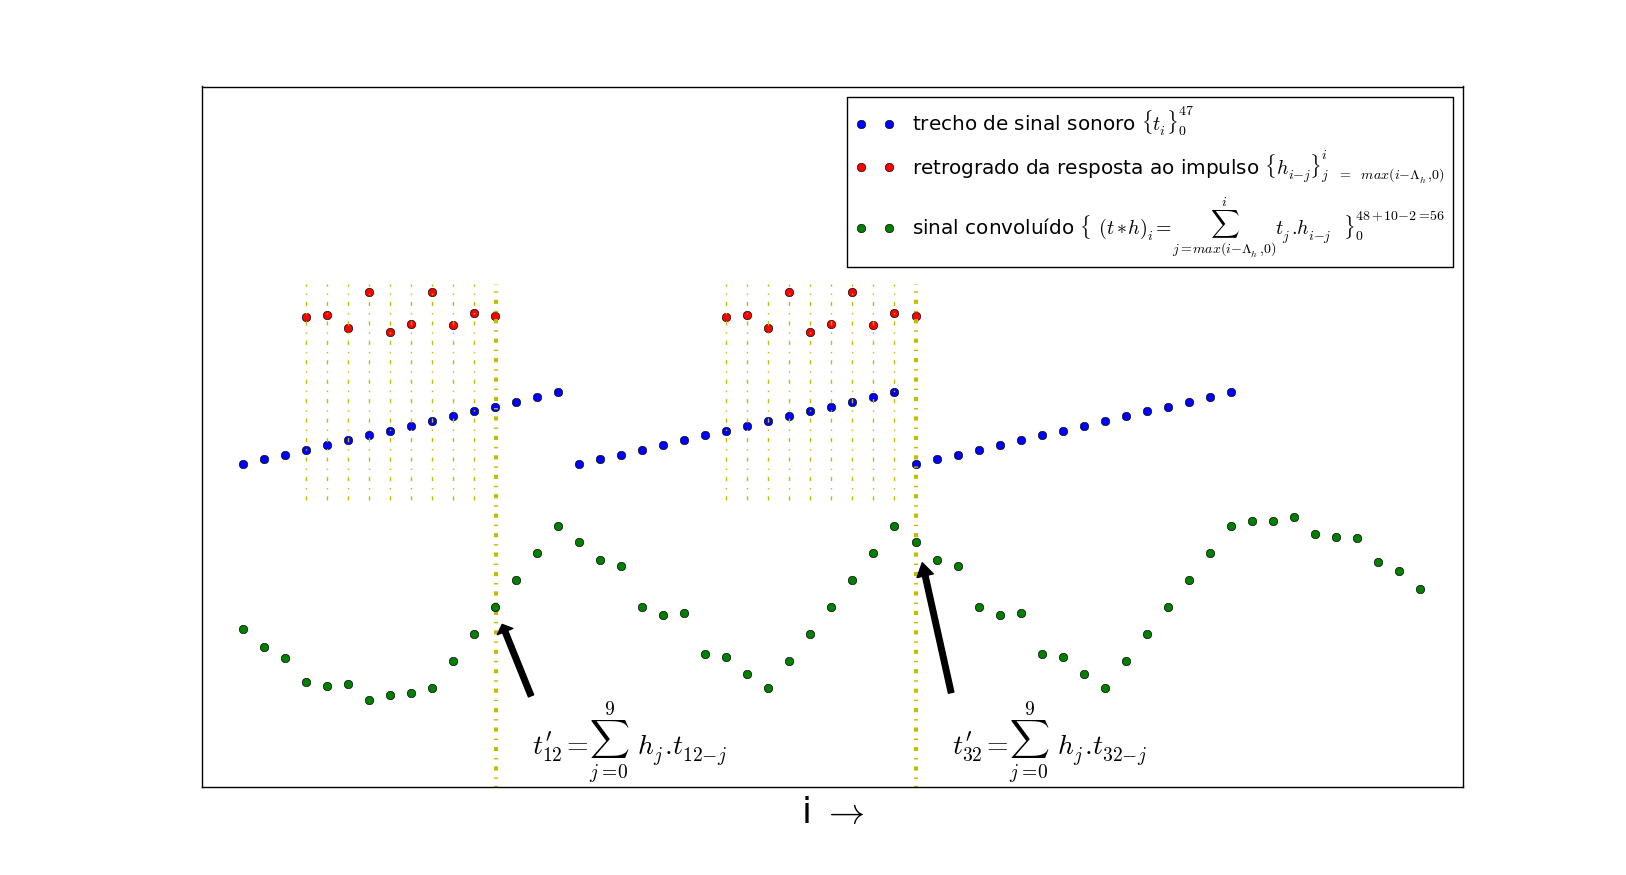
\includegraphics[width=\textwidth]{figuras/convolucao______}
        \label{fig:conv}
\end{figure}


Com este procedimento podemos aplicar reverberadores, equalizadores, delays
e vários outros tipos de filtros para fins de tratamento sonoro ou
efeitos musicais/artísticos.
 
Para a obtenção da resposta ao impulso, pode-se recorrer a medições
físicas ou à síntese direta do filtro. Para citar um exemplo
de medições diretas, uma resposta ao impulso para a aplicação
de reverberação pode resultar da gravação acústica do ambiente ao disparar
um estalo (cuja gravação se aproxima da resposta ao impulso diretamente) ou ao disparar uma
varredura de frequência (cuja gravação se aproxima da resposta em frequência).
Ambas resultam em respostas ao impulso
que, convoluídas com a sequência sonora, resultam na própria sequência
com uma reverberação que se assemelha à reverberação do ambiente 
em que ocorreu a medição.

Como exemplo de resposta ao impulso sintetizadas, pode-se
descrever um perfil espectral, realizar a transformada inversa
de fourier e convoluir o resultante com o som, realizando
uma filtragem cujo perfil é próximo ao especificado inicialmente. Note que este procedimento funciona particularmente bem se for grande o número de amostras utilizadas para especificar o perfil espectral do filtro\footnote{O que resulta em mais processamento computacional.}.

Outro exemplo simples e útil vem do deslocamento temporal causado pela convolução com o impulso deslocado. Assim, podemos aplicar de linhas de \emph{delays} através
da convolução do som com uma resposta ao impulso que possui um impulso
em cada reincidência do som na linha de delays intensionada.
Para ilustrar essa aplicação, dispomos a figura~\ref{fig:delays}
em que pode-se observar o deslocamento causado pela convolução
com o impulso. Dependendo da densidade dos impulsos, o resultado
é de caráter rítmico (20 impulsos por segundo ou menos) ou de amálgama
sonoro (20-40 impulsos por segundo ou mais). Neste último caso,
ocorrem processos tipicamente vinculados à síntese granular e às
equalizações.

\begin{figure}[h!]
    \centering
    \caption{Convolução com o impulso e linhas de delays}
        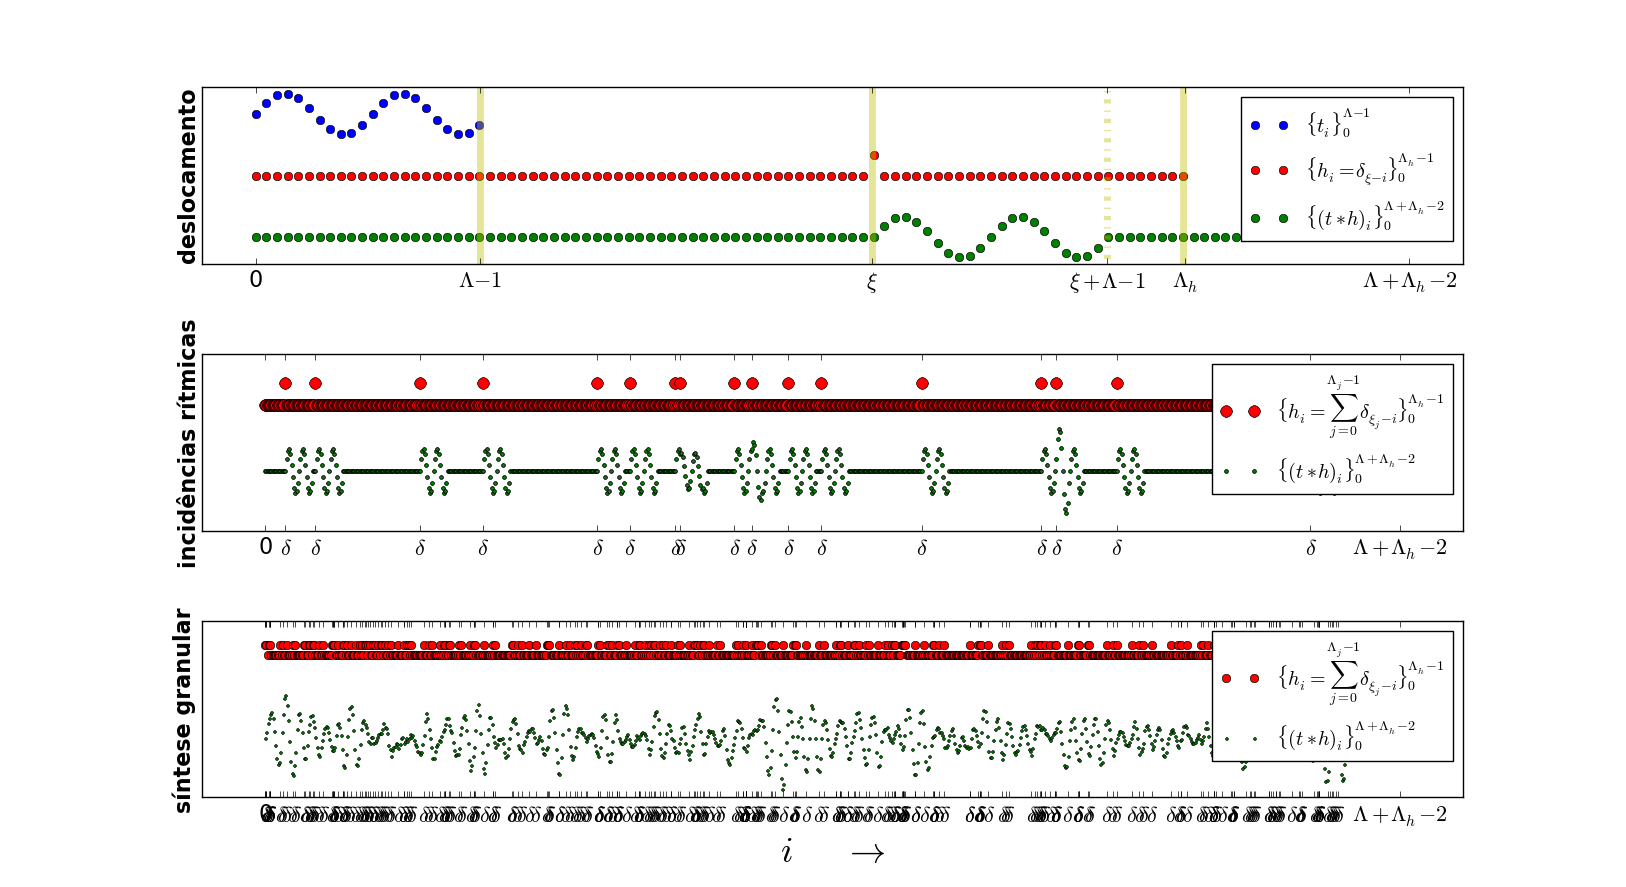
\includegraphics[width=\textwidth]{figuras/delays__}
        \label{fig:delays}
\end{figure}


\item Filtros de resposta ao impulso infinita (IIR)

Esta classe de filtros é
conhecida pela sigla IIR (do inglês Infinite Impulse Response)
e é caracterizada por possuir uma representação temporal
infinita, i.e. a resposta ao impulso não converge para zero. Sua aplicação é usualmente feita pela equação
a diferenças:

\begin{equation}
t_i' = \frac{1}{b_0}\left ( \sum_{j=0}^Ja_j . t_{i-j} - \sum_{k=1}^Kb_k . t_{i-k}' \right )
\end{equation}

com $b_0=1$ na grande maioria dos casos pois basta normalizarmos as variáveis
resultando em filtro idêntico: $a_j'=\frac{a_j}{b_0}$ e $b_k'=\frac{b_k}{b_0} \Rightarrow b_0' = 1$.

Apontamos filtros IIR bastante simples, úteis e usuais abaixo. Existem
diversos métodos e ferrametas para a elaboração de filtros IIR
e esta é uma seleção com fins didáticos e para consulta futura por
utilidade.
São filtros de primeira e segunda ordem bem comportados cujas
filtragens realizadas dispomos na figura~\ref{fig:iir}.

\begin{figure}[h!]
    \centering
    \caption{Filtragens realizadas pelos filtros IIR das equações \ref{eq:passa-baixas}, \ref{eq:passa-altas}, \ref{eq:passa-banda} e \ref{eq:rejeita-banda}}
        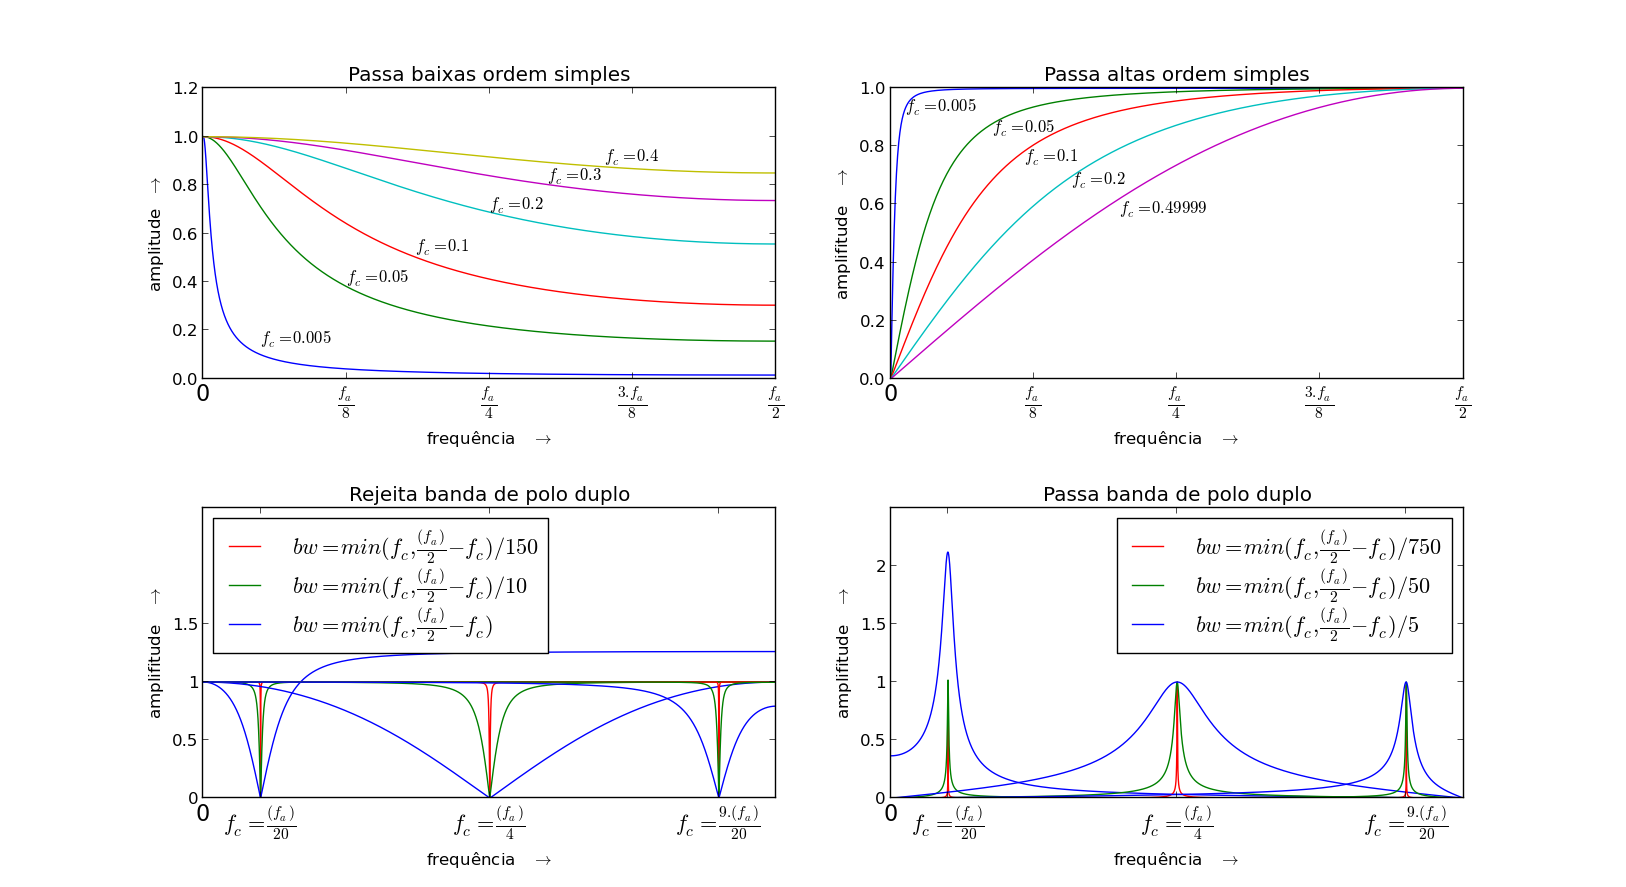
\includegraphics[width=\textwidth]{figuras/iir___}
        \label{fig:iir}
\end{figure}

No caso dos filtros de ordem simples, a frequência de corte $f_c$ é onde 
o filtro realiza uma atenuação de $-3dB \approx 0.707 $ da amplitude original.
No caso dos filtros passa e rejeita banda, esta mesma atenuação é
resultado de duas especificações: $f_c$ (neste caso melhor compreendida como 'frequência central') e a largura de banda $bw$
pois em ambas as frequências $f_c \pm bw$ há uma atenuação de $\approx 0.707$ da amplitude original.

Observe que existe amplificação do som no caso dos filtros passa e rejeita banda quando a frequência
de corte é baixa e a largura de banda é grande o suficiente. Nos agudos, estes filtros apresentam
somente um desvio do perfil esperado, expandindo a envoltória um pouco mais do lado grave da banda em
evidência.

Para conseguir filtros cujas respostas em frequência possuem outras envoltórias (para o módulo),
o recurso mais simples a esta altura
é fazer cascata destes filtros aplicando-os sucessivamente.

Outra possibilidade é usar alguma receita de filtro
biquad\footnote{Abreviação
de 'biquadrado' pois sua função de transferência possue dois polos e dois zeros, i.e. sua
forma normal consiste em dois polinômios quadráticos formando uma fração
$\mathbb{H}(z)=\frac{a_0+a_1.z^{-1}+a_2.x^{-2}}{1+ b_1.z^{-1} +b_2 . z^{-2}}$.}
ou rotinas para cálculo de coeficientes
de filtros Chebichev\footnote{Filtros Butterworth e Elípticos podem
ser considerados como casos específicos dos Filtros do tipo Chebichev~\cite{Openheim,smith}.}.
Ambas as possibilidades são exploradas
por títulos em nossas referências, em especial recomendamos~\cite{JOSFM,smith} e na coleção de filtros da comunidade \emph{Music-DSP}, da Universiade de Columbia~\cite{music-dsp}.
Para uma exposição aprofundada do assunto, recomendamos~\cite{Openheim}.

\end{itemize}

\begin{enumerate}
\item Passa-baixas de polo simples com gráfico do canto superior esquerdo da figura~\ref{fig:iir}. A fórmula geral tem
por referência da frequência de corte $f_c \in (0,\frac{1}{2})$,
fração da frequência de amostragem $f_a$
em que há aproximadamente uma atenuação de $3dB$.
Calculamos os coeficientes do filtro IIR
$a_0$ e $b_1$ 
através da variável intermediária: $x \in [0,1]$:

\begin{equation}\label{eq:passa-baixas}
\begin{split}
x & =e^{-2\pi f_c} \\
a_0 & =  1-x \\
b_1 & =  x
\end{split}
\end{equation}

\item Passa-altas de polo simples com gráfico do canto superior direito da figura~\ref{fig:iir}. A fórmula geral,
com frequência de corte $f_c \in (0,\frac{1}{2})$, é calculada através da variável
intermediária $x \in [0,1]$:


\begin{equation}\label{eq:passa-altas}
\begin{split}
x & =e^{-2\pi f_c} \\
a_0 & =  \frac{x+1}{2} \\
a_1 & =  -\frac{x+1}{2} \\
b_1 & =  x
\end{split}
\end{equation}


%\item Passa-banda
%\item Rejeita-banda
\item Nó (\emph{notch filter}). Este filtro é parametrizado
pela frequência central\footnote{Não
confundir com a frequência de corte também notada aqui por $f_c$ nos filtros passa baixas e passa altas.} $f_c$
e a largura de banda $bw$
($f_c \pm bw$ resulta em 0.707 da amplitude, i.e. atenuação de $3dB$),
ambos dados como fracoes de $f_a$, portanto $f,\; bw \in (0,0.5)$.
Por conveniência definimos as variáveis auxiliares $K$ e $R$ como:

\begin{equation}
\begin{split}
R & = 1 - 3BW \\
K & = \frac{1-2R\cos(2\pi f_c) + R^2}{2 - 2 \cos (2 \pi f_c)}
\end{split}
\end{equation}

A partir das quais temos dois filtros. O filtro passa banda que dispomos no canto inferior esquerdo da figura~\ref{fig:iir}:

\begin{equation}\label{eq:passa-banda}
\begin{split}
a_0 & =  1 - K \\
a_1 & =  2(K-R)\cos (2\pi f) \\
a_2 & =  R^2-K \\
b_1 & =  2R \cos (2\pi f) \\
b_2 & =  -R^2
\end{split}
\end{equation}

e o filtro rejeita banda:

\begin{equation}\label{eq:rejeita-banda}
\begin{split}
a_0 & =  K \\
a_1 & =  -2K\cos (2\pi f) \\
a_2 & =  K \\
b_1 & =  2R \cos (2\pi f) \\
b_2 & =  -R^2
\end{split}
\end{equation}

disposto na parte inferior esquerda da figura~\ref{fig:iir}.

%\item Biquad: pela especificação de uma frequência central, da qualidade
%e da intensidade do filtro, este filtro é simples e usual para áudio,
%permitindo ajustes mais finos. Diversas receitas podem ser encontradas
%na literatura, recomendamos especialmente as diferentes especificações
%em ~\ref{musicDSP} e ~\ref{dspguide}.

\end{enumerate}

\subsubsection{Ruídos}
De forma geral, os sons sem altura definida 
são chamados ruídos~\cite{Lacerda}.
Estes sons estão presentes como constituintes importantes dos sons musicais de altura definida,
como os ruídos presentes nas notas do piano, do violino, etc. Além disso, os instrumentos
de percussão, em grande parte, não possuem altura definida e seus sons
são muitas vezes compreendidos como ruídos~\cite{Roederer}. Na música eletrônica (incluindo
a eletroacústica), os ruídos possuem usos amplos, diversificados e comumente
idiomáticos~\cite{Cook}.

A ausência de uma altura definida é fruto da ausência de uma organização harmônica perceptível nas componentes senoidais que formam o som. Assim, pode-se inferir
as incontáveis possibilidades de gerar ruídos. A mais imediata é a utilização
de valores aleatórios para a geração da sequência sonora $T_i$. Este
é um método atraente, visto a disponibilidade
das consagradas distribuições de probabilidade em diversas linguagens de programação,
mas os resultados não são tão úteis, tendendo geralmente ao ruído branco
e com difíceis previsões do espectro resultante~\cite{Cook}.

Outra possibilidade é a geração de ruído através do espectro desejado. A partir
dele, executamos a transformada inversa de Fourier. Neste caso, é importante
que realizemos a distribuição espectral com cuidado pois queremos um perfil
do módulo do espectro e a fase é aleatória\footnote{Caso utilizemos a mesma fase
(ou fases com forte correlação) para
as componentes envolvidas, o som sintetizado possuirá energia bastante concentrada
em alguns trechos.}. Veja a figura~\ref{fig:ruidos} e o código Python que a gerou para uma implementação.


\begin{figure}[htpq!]
    \centering
    \caption{Ruídos coloridos realizados através das equações~\ref{eq:branco}, \ref{eq:rosa}, \ref{eq:marrom}, \ref{eq:azul}, \ref{eq:violeta}: espectros e ondas sonoras resultantes}
        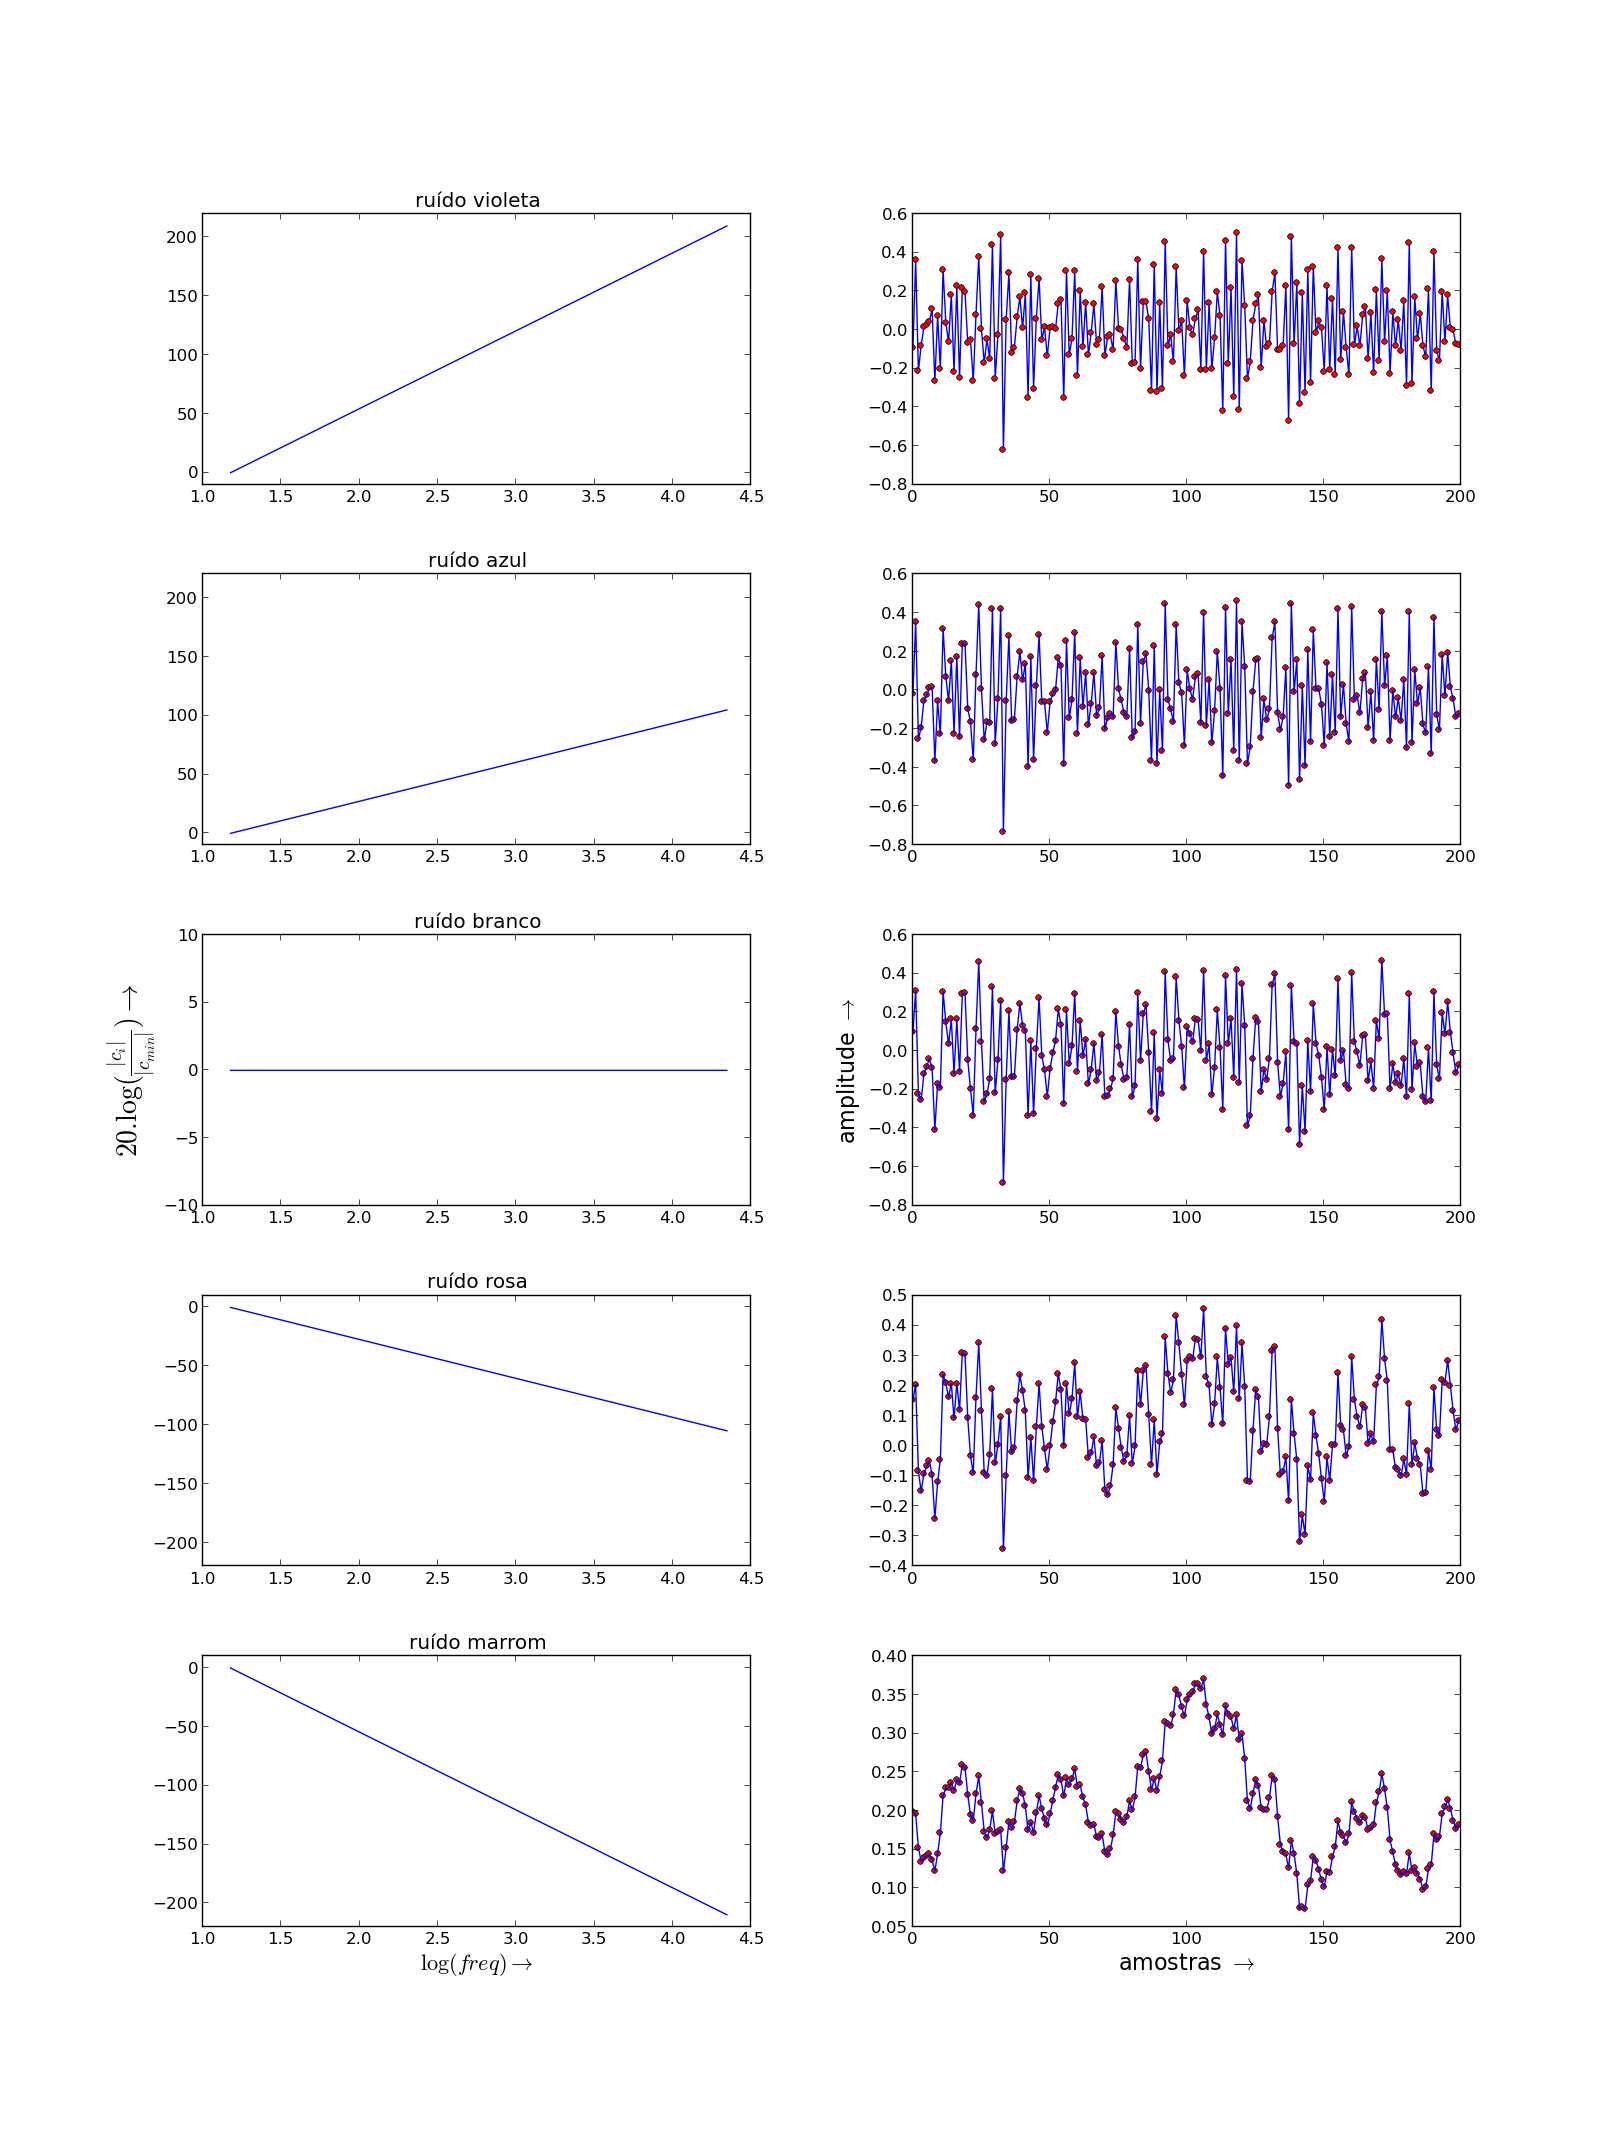
\includegraphics[width=\textwidth]{figuras/ruidos___}
        \label{fig:ruidos}
\end{figure}


Abaixo elencamos alguns ruídos de espectros estáticos. São chamados \emph{coloridos} por terem sido associados a cores. 

\begin{itemize}

\item O ruído branco deve seu nome por possuir energia distribuida
igualmente por todas as frequências. Podemos obter a realização
do ruído branco com a transformada inversa dos seguintes coeficientes:


\begin{equation}\label{eq:branco}
\begin{split}
c_0 & =0 \quad \text{pois não queremos bias} \\
c_i & =e^{j.x}\;,\;\; j^2=-1 \;, \;\; x \; \text{randômico} \; \in \; [0,2\pi]\;,\;\; i \; \in \; \left[1, \, \frac{\Lambda}{2}-1\right] \\
c_{\Lambda/2} & = 1 \quad\quad \text{(se $\Lambda$ par)}\\ 
c_i & = c_{\Lambda - i}^*\;,\;\; \text{para}\;  i \; > \;  \frac{\Lambda}{2}
\end{split}
\end{equation}

O valor de $c_i$ calculado pela exponencial é apenas um artifício para resultar em módulo unitário e fase aleatória.
Já $c_{\Lambda/2}$ é sempre puramente real (como vimos na sessão anterior).

\item O ruído rosa possui uma queda de $3dB$ por oitava. Este ruído é muito usual no teste de equipamentos e montagens de aparelhos além de presença destacada na natureza~\cite{Roederer}. 

\begin{equation}\label{eq:rosa}
\begin{split}
f_{\text{min}} & \approx 15 Hz \\
f_i & = i \frac{f_a}{\Lambda} \;, \;\; \quad i \;\leq\; \frac{\Lambda}{2},\;\; i\;\in\;\mathbb{N}  \\
\alpha_i & = (10^{-\frac{3}{20}})^{\log _2 \left ( \frac{f_i}{f_{\text{min}}} \right )}  \\
c_i & =0\;,\;\; \forall \; i \; : f_i<f_{\text{min}} \\
c_i & =e^{j.x} . \alpha_i\;,\;\; j^2=-1 \;, \;\;\  x \;\; \text{randômico} \; \in \; [0,2\pi]\;,\;\; \forall \; i \; : f_{\text{min}} \le f_i < f_{\lceil \Lambda/2-1 \rceil}  \\
c_{\Lambda/2} & = \alpha_{\Lambda/2} \quad\quad \text{(se $\Lambda$ par)}\\ 
c_i & = c_{\Lambda - i}^*\;,\;\; \text{para}\;  i \; > \;  \Lambda/2
\end{split}
\end{equation}

A frequência mínima $f_{\text{min}}$ pode ser escolhida com base no limite da audição, pois não escutamos como altura de um som uma frequência absoluta abaixo de $\approx\; 20Hz$.

O resto dos ruídos podem ser feitos com base neste procedimento descrito para 
o ruído rosa. Basta que modifiquemos alguns detalhes. Em especial a equação que define $\alpha_i$.

\item O ruído marrom deve seu nome ao Robert Brown, que descreveu o movimento browniano.
Embora esta origem seja um tanto díspar do que poderiamos considerar motivo para uma associaçãocom a cor marrom, o ruído sonoro ficou consagrado com este nome. De qualquer forma, é bastante comum declarar satisfatória a associação do ruído com a cor marrom, dados os ruídos branco e rosa mais estridentes e relacionados a cores mais intensas~\cite{marrom}.

O que caracteriza este ruído é a queda de $6dB$ por oitava. Desta forma, basta modificarmos a equação de $\alpha_i$ 
no conjunto \ref{eq:rosa} para:

\begin{equation}\label{eq:marrom}
\alpha_i=(10^{-\frac{6}{20}})^{\log _2 \left( \frac{f_i}{f_{\text{min}}} \right )}
\end{equation}

\item Ruído azul é aquele em que há um ganho de $3dB$ por oitava em uma banda limitada. Para
a síntese deste ruído, basta estipularmos a frequência mínima $f_{\text{min}}$ e a frequência
máxima $f_{\text{máx}}$. Assim, também com base no conjunto de equações \ref{eq:rosa}, 
basta atentarmos para as sequintes identidades:

\begin{equation}\label{eq:azul}
\begin{split}
\alpha_i & = (10^{\frac{3}{20}})^{\log _2 \left ( \frac{f_i}{f_{\text{min}}} \right )} \\
c_i & =0\;,\;\; \forall \; i \; : f_i<f_{\text{min}} \;\; \text{ou} \;\; f_i>f_{\text{máx}} \\
\end{split}
\end{equation}

\item O ruído violeta é similar ao ruído azul, mas o ganho é de $6dB$ por oitava:

\begin{equation}\label{eq:violeta}
\alpha_i = (10^{\frac{6}{20}})^{\log _2 \left ( \frac{f_i}{f_{\text{min}}} \right )} \;\;, \quad f_{\text{min}} \approx 15 Hz \\
\end{equation}

\item O ruído preto possui perdas maiores que $6dB$ por oitava, assim:

\begin{equation}\label{eq:preto}
\alpha_i=(10^{-\frac{\beta}{20}})^{\log _2 \left( \frac{f_i}{f_{\text{min}}} \right )}\;\;, \quad \beta > 6
\end{equation}



\item Um pouco diferente dos exemplos acima é o ruído cinza, definido como
um ruído branco sujeito a uma das curvas iso-audíveis. Como estas curvas são resultados
experimentais, precisamos neste caso da curva para a realização dos fatores multiplicativos
$\alpha_i$.

\end{itemize}

Com base nestes ruídos expostos podemos prever a infinidade de ruídos utilizados. Importante
neste momento é entender que foram expostos somente ruídos com espectro estático. Existem classificações
de ruídos com variações do espectro no decorrer do tempo. Existem também ruídos que
são fundamentalmente transientes, como os clicks e os chirps. O primeiro é modelado
facilmente por um impulso relativamente isolado, enquanto o segundo é uma varredura rápida de 
alguma banda de frequência~\cite{Cook}.

Os ruídos das equações \ref{eq:branco}, \ref{eq:rosa}, \ref{eq:marrom},
\ref{eq:azul}, \ref{eq:violeta} estão na figura \ref{fig:ruidos}. Vale notar
que os espectros foram feitos com a mesma fase nos coeficientes, de forma que
pode-se observar a contribuição dos harmônicos agudos no traçado geral dado
pelas frequências graves e muito explícito no ruído marrom.


\subsubsection{Usos musicais parte 1: trêmolo e vibrato, AM e FM}

Enquanto o vibrato é uma variação periódica de altura (frequência),
o tremolo é uma variação periódica de volume (intensidade).

Iniciemos pelo vibrato. Para realizarmos o caso mais geral, façamos uma sequência $t_i'$
de frequência $f'$ com o auxílio
de uma segunda tabela $\widetilde{M}_i$ de tamanho $\widetilde{\Lambda}_M$ que apresente também
um período de onda que oscila entre $[-1,1]$. Descrevemos uma sequência sonora $t_i^{vbr(f',\,\nu)}$ com
um vibrato de frequência $f'$ e profundidade  $\mu$ (quantos herz é a oscilação no pico superior)
ou $\nu$ (amplitude do vibrato em semitons) da seguinte forma:


\begin{equation}\label{vbrGamma}
\gamma_i'=\left \lfloor i f' \frac{\widetilde{\Lambda}_M}{f_a} \right \rfloor
\end{equation}

\begin{equation}\label{vbrAux}
t_i'=\widetilde{m}_{\gamma_i' \;\% \widetilde{\Lambda}_M}
\end{equation}

\begin{equation}\label{vbrF}
f_i=f \left ( \frac{f + \mu }{f} \right )^{t_i'}=f . 2^{t_i'\frac{\nu}{12}}
\end{equation}

\begin{equation}\label{vbrGamma}
\Delta_{\gamma_i}=f_i\frac{\widetilde{\Lambda}}{f_a} \quad \Rightarrow \quad \gamma_i = \left \lfloor \sum_{j=0}^{i} f_i \frac{\widetilde{\Lambda}}{f_a} \right \rfloor = \left \lfloor \sum_{j=0}^{i} \frac{\widetilde{\Lambda}}{f_a}f \left ( \frac{f + \mu }{f} \right )^{t_i'}  \right \rfloor= \left \lfloor \sum_{j=0}^{i} \frac{\widetilde{\Lambda}}{f_a}f . 2^{t_i'\frac{\nu}{12}}  \right \rfloor
\end{equation}

\begin{equation}\label{vbrT}
T_i^{f, vbr(f')}=\{ t_i^{f,vbr(f')} \}_0^{\Lambda-1}=\{ \widetilde{l}_{\gamma_i \%\; \widetilde{\Lambda} } \}_0^{\Lambda-1}
\end{equation}


\begin{figure}[h!]
    \centering
    \caption{Espectrograma de um som com vibrato senoidal de $3Hz$ e profundidade de uma oitava em uma dente de serra de $1000Hz$}
        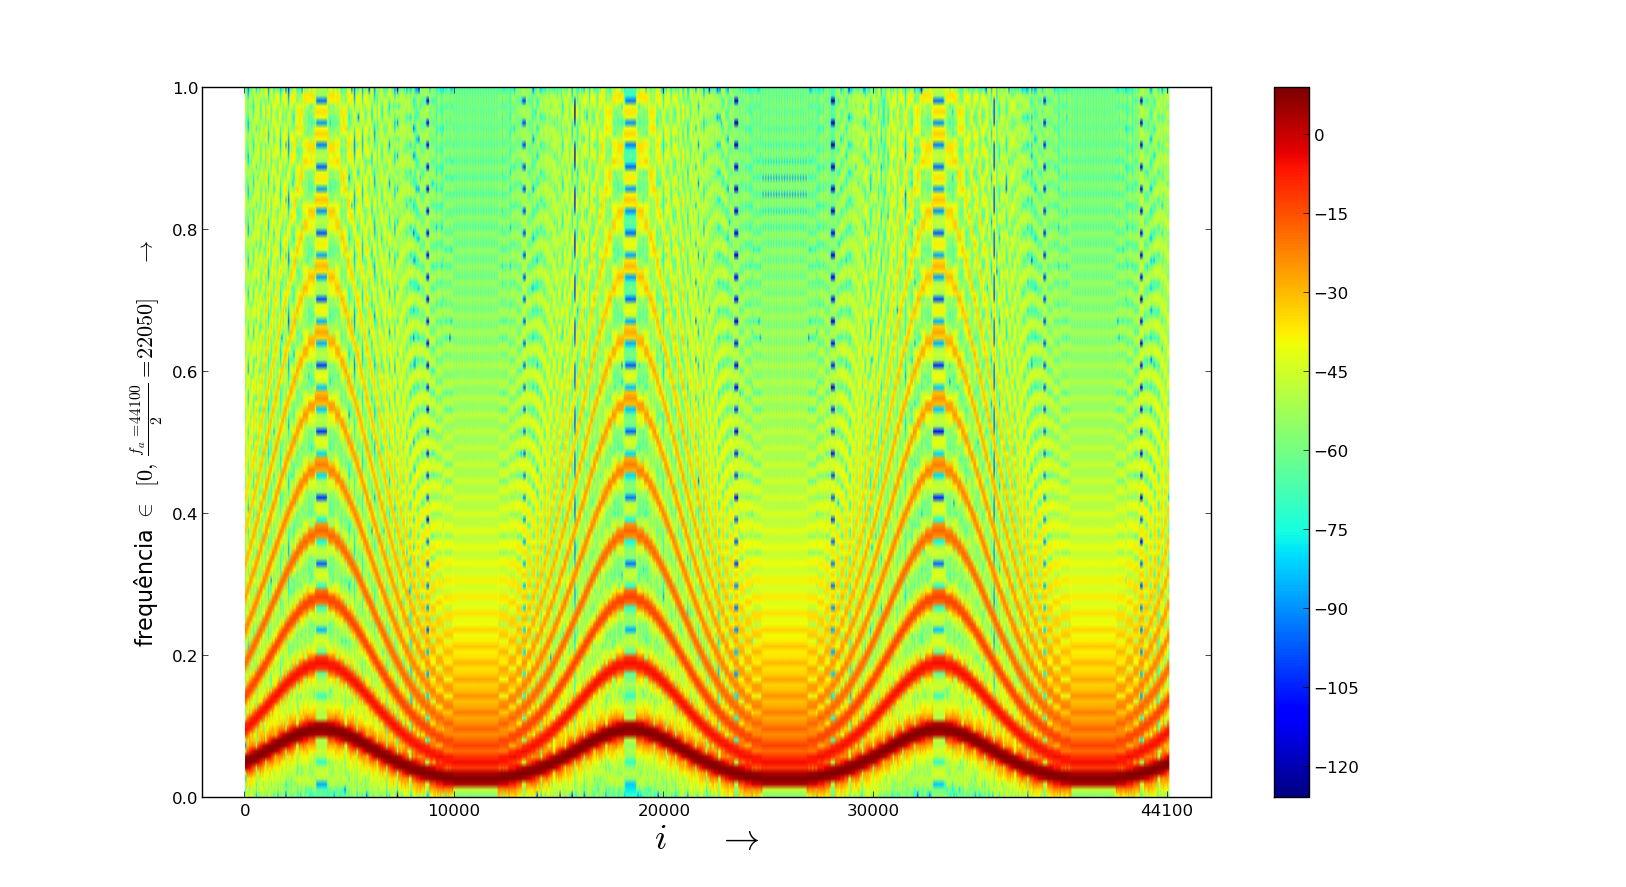
\includegraphics[width=\textwidth]{figuras/vibrato___}
        \label{fig:vibrato}
\end{figure}

Para a correta realização do vibrato, é importante atenção para as duas tabelas e sequências.
A tabela $\widetilde{M}_i$ de tamanho $\widetilde{\Lambda}_M$ e a sequência de índices $\gamma_i'$ formam a sequência $t_i'$
 que é o padrão da oscilação da frequência enquanto
a tabela $\widetilde{L}_i$ de tamanho $\widetilde{\Lambda}$ e a sequência de índices $\gamma_i$ formam $t_i$ que é o som em si.
As variáveis $\mu$ e $\nu$ quantificam a intensidade do vibrato: $\mu$ é uma medida direta da quantidade
de Herz envolvidos no limite superior da oscilação e $\nu$ é a medida direta de semitons envolvidos na oscilação ($2\nu$ é o número de semitons entre os picos superioes e inferiores de oscilação da frequência do som $t_i$ causada pelo vibrato).
Note que $\nu=\log_{2}\frac{f+\mu}{f} $ é conveniente neste caso pois o aumento máximo de frequência
não equivale à diminuição máxima, mas a variação de semitons se mantém.

A Figura \ref{fig:vibrato} é o espectrograma de um vibrato artificial de uma nota em
$1000Hz$ (entre um si e um dó) e cujo desvio da frequência atinge uma oitava
para cima e para baixo. Note o padrão senoidal do vibrato e as compontentes harmônicas
da dente de serra. Qualquer forma de onda pode
ser utilizada para gerar o som e o padrão de oscilação do vibrato, o que é tão crucial para os usos musicais quanto a
frequência de oscilação e o desvido de altura envolvido\footnote{O desvio de altura
é chamado profundidade do vibrato e é dado por conveniência em semitons ou cents.}. Estas qualidades não são praticáveis em instrumentos musicais tradicionais, introduzindo novidade nas possibilidades musicais.

O caso do tremolo é semelhante e $f'$, $\gamma_i'$ e $t_i'$ permanecem os mesmos. Calculamos
a sequência de amplitudes a serem multiplicadas pela sequência original $t_i$ da
sequinte forma:

\begin{equation}\label{trA}
a_i=10^{t_i' \frac{V_{dB}}{20}} = a_{\text{máx}}^{t_i'}
\end{equation}

\begin{equation}\label{trT}
T_i^{tr(f')}=\{ t_i^{tr(f')} \}_0^{\Lambda-1}=\{ t_i . a_i \}_0^{\Lambda-1}=\{t_i .10^{t_i' \frac{V_{dB}}{20}}    \}_0^{\Lambda-1}=\{t_i . a_{\text{máx}}^{t_i'}\}_0^{\Lambda-1}
\end{equation}

Onde $V_{dB}$ é a profundidade da oscilação em decibels do trêmolo e $a_{\text{máx}}=10^{\frac{V_{dB}}{20}}$
 é o ganho máximo de amplitude envolvido.
A medição em decibels é bastante pertinente pois o aumento máximo de amplitude
não equivale à diminuição máxima relacionada, enquanto a diferença em decibels se mantém.

A figura~\ref{fig:tremolo} mostra a amplitude das sequências $\{a_i\}_0^{\Lambda-1}$ e $\{t_i'\}_0^{\Lambda-1}$
para três oscilações de um trêmolo com forma da dente de serra. A curvatura é devido à progressão logarítmica de
intensidade. A frequência do trêmolo é de $1,5Hz$ pois $f_a=44,1kHz \; \Rightarrow \; \text{duração} = \frac{i_{\text{máx}}=82000}{f_a}= 2s \; \Rightarrow \; \frac{3\text{oscilações}}{2s}=1,5$ oscilações por segundo ($Hz$). 

A peça \emph{vibra e treme} explora estes recursos dos tremolos e vibratos
com frequências $f'$
e profundidades ($\nu$ e $V_{dB}$) diferentes. Usadas em associação e isoladamente e com variações progressivas dos parâmetros. A peça desenvolve também uma comparação entre os vibratos e tremolos que se desenvolvem em escala logarítmica e em escala linear.


\begin{figure}[h!]
    \centering
    \caption{Tremolo de profundidade $12dB$ com padrão oscilatório de uma dente de serra em $1,5Hz$ em uma senoide de $40Hz$ (considerada taxa de amostragem $f_a=44,1kHz$)}
        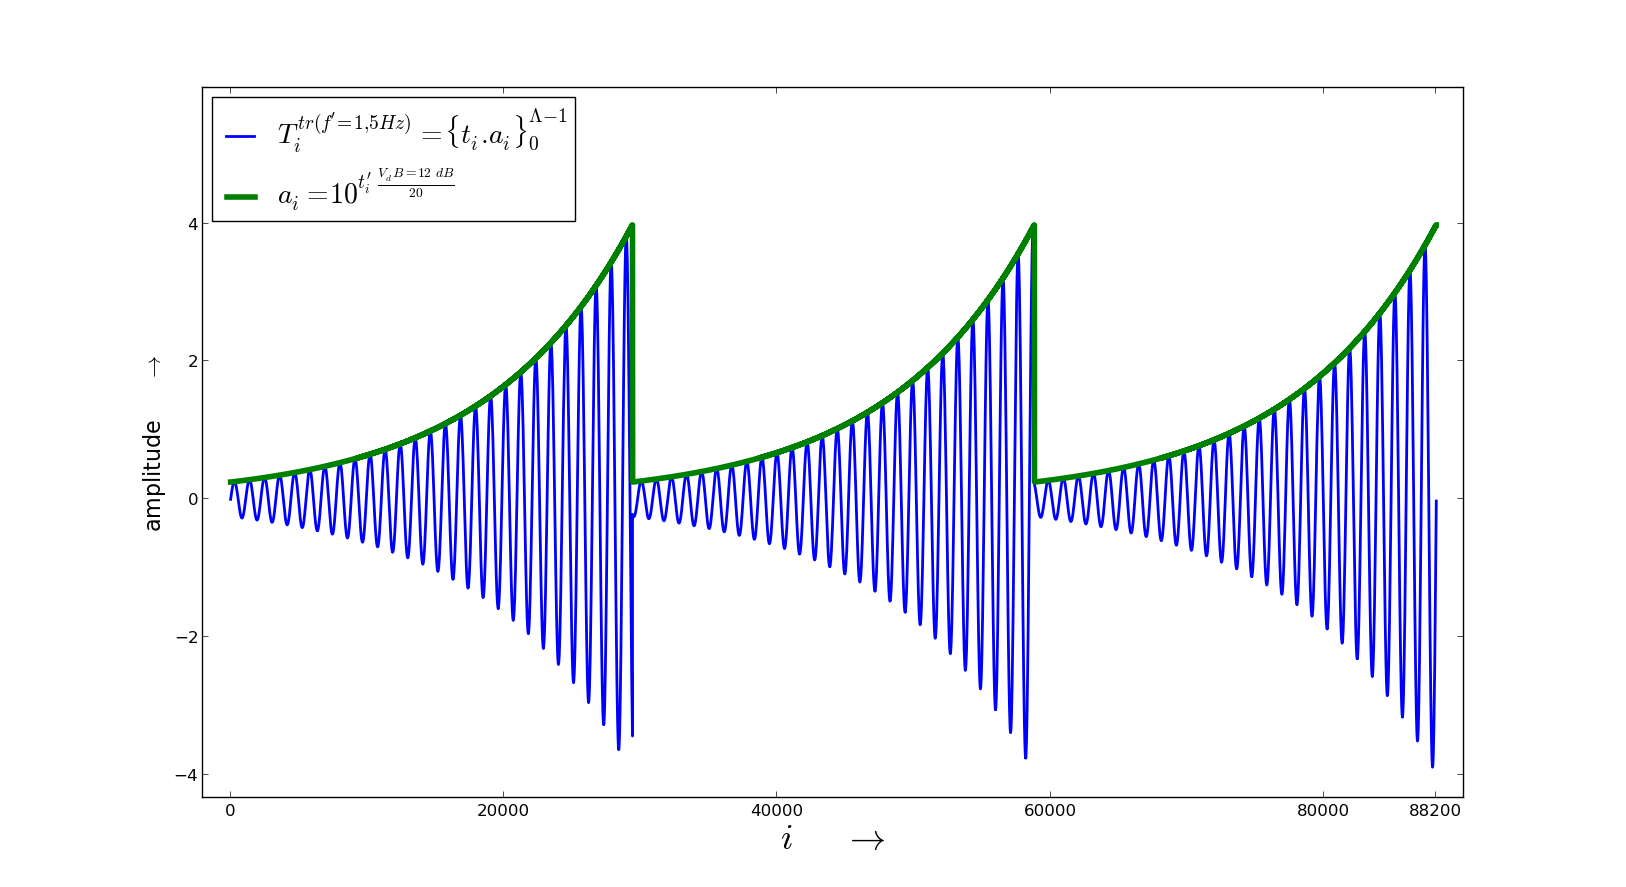
\includegraphics[width=\textwidth]{figuras/tremolo}
        \label{fig:tremolo}
\end{figure}

As equações ~\ref{vbrT}, ~\ref{vbrGamma}, ~\ref{vbrF} e ~\ref{vbrAux}
são utilizadas para síntese nos casos em que $f'$ é
maior que $20Hz$ e as oscilações de frequência resultam em padrões complexos
de componentes espectrais harmônicas e não harmônicas. É a chamada síntese
por frequência modulada (FM).

As equações ~\ref{trA} e ~\ref{trT}
(junto às ~\ref{vbrT} e ~\ref{vbrGamma} para a realização da sequência auxiliar $t_i'$) 
resultam na síntese chamada de amplitude modulada (AM)
quando $f'$ é maior que $20Hz$\footnote{As sínteses
FM e AM são técnicas com diversas amplicações na música e também em outras áreas,
especialmente conhecidos são os usos telecomunicações para transferência de informações
via ondas eletromagnéticas. O leitor interessado pode visitar os itens relacionados
da nossa bibliografia para uma abordagem musical (veja especialmente ~\ref{} e ~\ref{})
ou aproveitar nossa abordagem breve sobre o assunto nos usos musicais desta sessão, logo abaixo.}.

----

Algo interessante ocorre se aumentarmos progressivamente $f'$.
Primeiramente o limiar de frequência
para audição do fenômeno sonoro como
altura ($\approx 20Hz$) gera rugosidades para
ambos tremolos e vibratos. A sequência \emph{Rugosidades}
explora este limiar com concomitâncias de tremolos e vibratos na mesma
voz, com intensidades e formas de onda diferentes.

Se continuarmos aumentando a frequência, deixamos de ouvir estas oscilações
como eventos identificáveis. Neste caso, as oscilações se apresentam na forma de espectro
audível como altura, $f'$ e a forma de onda realizam alterações espectrais no som
original $T_i$ de formas diferentes para os tremolos e para os vibratos, são as 
chamadas sínteses AM (Amplitude Modulation) e FM (Frequency Modulation).
Estas são técnicas muito poderosas e conhecidas, com aplicações em sintetizadores
históricos como o Yamaha XXX e com aplicações fora da música, como em telecomunicações
(ex. radios AM e FM).

Para nosso caso, em resumo, podemos entender a síntese FM através do caso entre senoides
e decompor os sinais em seus espectros de Fourier (i.e. senoidais) para casos mais complexos.
Assim, a síntese FM realizada com um vibrato de frequência $f'$ em um som $T_i$ de frequência $f$
e duração $\Delta$ segundos (assumimos $\Lambda = \lfloor \Delta . f_a \rfloor $ amostras)
gera bandas centradas em $f$ e distantes $f'$ entre si:

\begin{equation}\label{eq:fmEsp}
\begin{split}
\{t_i'\}_0^{\Lambda -1} & = \left \{ \cos \left [f . 2 \pi \frac{i}{f_a-1} + \mu . sen \left ( f' . 2 \pi \frac{i}{ f_a -1 } \right ) \right ] \right \}_0^{\Lambda-1}  = \\
 & = \left \{ \sum_{k=-\infty}^{+\infty} J_k(\mu) \cos \left [ f . 2 \pi \frac{i}{f_a-1} + k . f' . 2 \pi \frac{i}{f_a-1} \right ]  \right \}_0^{\Lambda-1} = \\
 & = \left \{ \sum_{k=-\infty}^{+\infty} J_k(\mu) \cos \left [ (f+k.f') . 2 \pi \frac{i}{f_a-1} \right ]  \right \}_0^{\Lambda-1}
\end{split}
\end{equation}

onde 
\begin{equation}
J_k(\mu) = \frac{2}{\pi} \int_0^{\frac{\pi}{2}}\left [ cos \left (\overline{k}\;\frac{\pi}{2} + \mu . \sin w \right ) . cos \left ( \overline{k}\;\frac{\pi}{2} + k . w \right ) \right ] dw \quad , \quad \overline{k} = k \% 2 \;\;,\;\; k \in \mathbb{N}
\end{equation}
é a função de Bessel~\cite{BesselCCRMA,JOSFM}. Note que, nestas equações, a variação de frequência não respeita a progressão geométrica de frequência que acompanha a percepçao de altura. Caso utilizemos as equações~\ref{vbrF} teríamos uma distribuição diferente dos harmônicos. Para este fim, dispomos o APÊNDICE~\ref{cap:fmam} onde calculamos o conteúdo espectral da síntese FM feita com oscilações na escala logarítmica. De fato, como pode-se notar nos cálculos, o comportamento simples que torna a FM é privilégio das variações lineares utilizadas em~\ref{eq:fmEsp}.

O caso da modulação de amplitude (AM) é mais simples:

\begin{equation}\label{eq:am}
\begin{split}
\{t_i'\}_0^{\Lambda-1} & =\{(1+a_i) . t_i\}_0^{\Lambda-1}= \left \{ \left [ 1+M.\sin \left ( f'.2\pi\frac{i}{f_a -1} \right ) \right] . P .\sin \left ( f.2\pi\frac{i}{f_a -1} \right ) \right \}_0^{\Lambda-1} = \\
& = P.\sin \left( f.2\pi\frac{i}{f_a -1}  \right ) + \frac{P.M}{2} \left [ \sin \left( (f-f').2\pi\frac{i}{f_a -1}  \right ) + \sin \left( (f+f').2\pi\frac{i}{f_a -1}  \right ) \right ]
\end{split}
\end{equation}

Ou seja, o sinal resultante é o sinal original (chamada portadora, com conteúdos harmônicos como a senoide de frequência $f$)
e a reprodução de seu conteúdo espectral acima e abaixo da frequência
original, distantes na proporção de cada harmônico ($f'$) da moduladora.

 Além do comparativo qualitativo que é explorado entre as oscilações nas escalas diferentes, é uma ponte conveniente com as sínteses FM e AM.

\subsubsection{Usos musicais livres}
A este ponto as possibilidades musicais explodiram. Possuímos unidades
musicais com características próprias de altura (dada pela frequência),
tímbre (dada pela forma de onda),
volume (dada pela intensidade) e duração (dada pelo número de amostras).
Em uma nota, estas características podem ser consideradas
de forma absoluta ou tratadas ao longo de sua duração,
com a única excessão da duração em si.

Desta forma, os usos musicais que apresentamos é uma coleção de possibilidades
com o objetivo de exemplificar manipulações sonoras que resultem algo
musical, por razões variadas e aprofundadas na próxima sessão.

Uma primeira possibilidade interessante é o estabelecimento de vínculos
entre os parâmetros do trêmolo e do vibrato e algum parâmetro da nota básica,
digamos a frequência. Assim, podemos estabelecer que quanto mais aguda é a nota,
mais alta é a frequência do vibrato e do trêmolo mas menor a sua profundidade.
Desta forma, tomando por base as equações \ref{vbrGamma}, \ref{vbrF} e \ref{trA}
podemos escrever:

\begin{equation}
\begin{split}
f^{vbr} = f^{tr} & = func_a(f) \\
\nu & = func_b(f) \\
V_{dB} & = func_c(f)
\end{split}
\end{equation}

Com $f^{vbr}$ e $f^{tr}$ sendo $f'$ nas equações de referência, ou seja, a frequência
de oscilação do vibrato e do tremolo utilizada na equação~\ref{vbrGamma}. Já $\nu$ e $V_{dB}$ são as profundidades
do vibrato e do tremolo, respectivamente. A montagem musical 
\emph{tremolos, vibratos e a frequência} explora
recursos como este e variações da forma de onda da oscilação. As possibilidades
são numerosas e ricas e, aliás, os tremolos e os vibratos naturais ocorrem
juntos, i.e. quase todo tremolo natural também apresenta oscilação de frequência
e vice versa.

Estas oscilações - aplicadas à amplitude, frequência, posição espacial - são ornamentos muito apreciados e possuem nomes
específicos. Em linguagem pianística,
os tremolos são ocorrências em que se alternam rapidamente 2 notas (com
casos de expansão do conceito), ou seja, seriam mais facilmente associados aos vibratos
segundo a nomenclatura aqui utilizada\footnote{Veja nosso glossário.}.

---------

Com relação à convolução, podemos estabelecer um pulso musical (a exemplo de um pulso BPM)
e distribuir impulsos no decorrer deste pulso, de forma a estabelecer métricas e rítmos\footnote{Lembrando
que a convolução com o impulso resulta no som deslocado ao instande de ocorrência do impulso}.
Por exemplo, se escolhemos 2 impulsos igualmente espaçados, estaremos fazendo uma
divisão binária básica do pulso. Se escolhemos dois sinais, um com 2 pulsos e outro com 3 pulsos,
ambos com os impulsos igualmente espaçados na duração do pulso, resultamos na manutenção
do pulso, com uma marcação rítmica usada tanto em divisões binárias quanto ternárias em diversos
estilos de música étnica e tradicional. 
Os próprios valores absolutos destes impulsos resultam em proporções entre as amplitudes dos sinais
convoluídos.
Exploramos este recurso da métrica
estabelecida pela convolução com impulsos na sequência musical \emph{trenzinho de caipiras impulsivos}.

Já com os filtros as possibilidades explodem ainda mais vertiginosamente. Pode-se convoluir um sinal para reverberá-lo, para
remover algum ruído, para gerar distorções ou tratamento com intuito estético mesmo. Por exemplo,
aplicando um filtro bassa banda em que deixamos passar somente entre $1kHz$ e $3kHz$, geramos um som
que parece de telefone ou de televisão antiga. Ao remover com alguma precisão somente
a frequência de oscilação da rede elétrica (usualmente $50Hz$ ou $60Hz$) e harmônicas, podemos remover
ruídos introduzidos pelos equipamentos de áudio utilizados. Um uso mais incrementado
e propriamente musical seria realizar filtragens em bandas específicas e usar estas bandas
pré estabelecida como um parâmetro adicional das notas.

Um recurso musicalmente forte é a filtragem dependente do tempo, no qual convém os filtros IIR, em que
os valores do filtro podem ser modificados - com algum cuidado - ao longo de sua aplicação. Cascatas
destes filtros podem realizar filtragens complexas e mais precisas. A montagem \emph{ruídos e faixas} explora
este recursos, realizando filtragens em ruídos diversos, com sequênciamento de disposição de bandas
e ruídos específicos, e filtragens que variam no tempo.

Um uso incrementado destes recursos todos seria a realização de um efeito chamado \emph{chorus}. Ao
exemplo do que ocorre com um coro de cantores, neste efeito o som é realizado com diversas pequenas modificações,
potencialmente aleatórias, em paramêtros como frequência central, presença (ou ausência) de vibrato
e trêmolo e suas características, equalizações, volume etc. Para o resultado final, estas versões do som
inicial é então mixado (ver equação \ref{eq:mixagem}). A peça \emph{chorus infantil} realiza chorus de formas
diferentes em sons diferentes.




\clearpage
\subsection{Organização de notas musicais em música}
Seja $ S=\{T_{i,1},T_{i,2}...T_{i,N}\} =\bigcup_{j \in [1,N]} T_{i,j} $ uma sequência de $N$ eventos
musicais. Para simplificar, sejam notas musicais estes eventos musicais.
Considerando $S$ como uma estrutura musical, existem diversas técnicas
para tornar estas estruturas interessantes e agradáveis.

\subsubsection{Afinação, escalas e acordes}
Quando dobramos a frequência, temos uma oitava ascendente $f_2=2f_1$.
Doze semitons equidistantes para o ouvido formam uma oitava,
portanto $f_2=2^{\frac{1}{12}}f_1$ forma um semitom ascendente.
O fator $\varepsilon=2^{\frac{1}{12}}$ forma uma grade de notas
no espectro audível, em que as frequências fundamentais possíveis
estão separadas por intervalos múltiplos de $\varepsilon$\footnote{Este
é um modelo idealizado, os intrumentos reais possuem desvios das frequências
fundamentais como citadas}.

Esta divisão da oitava em doze notas é o cânone da música ocidental clássica,
além de usos cerimoniais/religiosos e étnicos. Nesta afinação, chamada cromática
de temperamento igual, temos 5 divisões perfeitamente simétricas, consideradas
escalas pela simetria interna e usos fáceis que disso resultam. Descrevamos
as escalas como sequências de fatores aos quais $\varepsilon$ é elevado para resultar
no fator a ser multiplicado por $f_0$:

\begin{equation}
\begin{split}
\text{cromática} = E_i^c = \{e_i^c\}_0^{11} =  \{0,1,2,3,4,5,6,7,8,9,10,11\} = \{i\}_0^{11}\\
\text{tons inteiros} = E_i^t = \{e_i^t\}_0^{5} = \{0,2,4,6,8,10\} = \{2.i\}_0^{5} \\
\text{terças menores} = E_i^{tm} = \{e_i^{tm}\}_0^{3} = \{0,3,6,9\} = \{3.i\}_0^3 \\
\text{terças maiores} = E_i^{tM} = \{e_i^{tM}\}_0^{2} = \{0,4,8\} = \{4.i\}_0^2\\
\text{trítonos} = E_i^{tt} = \{e_i^{tt}\}_0^{1} = \{ 0, 6 \} = \{6.i\}_0^1
\end{split}
\end{equation}

Assim, a terceira nota da escala em tons inteiros com $f_0=200Hz$
é $f_3=\varepsilon^{e_3^t} . f_0 = 2^{\frac{6}{12}} . 200 \approxeq 282.843 Hz$. Estas
'escalas' ou padrões, geram estruturas estáveis pelas simetrias internas, e podem ser
repetidas de forma eficiênte e sustentada. Discutiremos mais sobre simetrias e voltaremos
a estas divisões da oitava por igual.

As escalas diatonicas também são facilmente especificadas, assim como
as escalas tonais maior e menor:


\begin{equation}
\begin{split}
\text{menor natural} = \text{modo eólico} = E_i^m = \{e_i^m\}_0^6 = \{0,2,3,5,7,8,10\} \\
\text{menor harmônica} = E_i^{mh} = \{e_i^{mh}\}_0^6 = \{0,2,3,5,7,8,11\} \\
\text{menor melódica} = E_i^{mm} = \{e_i^{mm}\}_0^{14} = \{0,2,3,5,7,9,11,12,10,8,7,5,3,2,0\} \\
\text{modo lócrio} = E_i^{mlo} = \{e_i^{mlo}\}_0^6 = \{0,1,3,5,6,8,10\} \\ 
\text{maior} = \text{modo jônico} = E_i^M = \{e_i^M\}_0^6 = \{0,2,4,5,7,9,11\} \\
\text{modo dórico} = E_i^{md} = \{e_i^{md}\}_0^6 = \{0,2,3,5,7,9,10\} \\
\text{modo frígio} = E_i^{mf} = \{e_i^{mf}\}_0^6 = \{0,1,3,5,7,8,10\} \\
\text{modo lídio} = E_i^{ml}=\{e_i^{ml}\}_0^6 = \{0,2,4,6,7,9,11\} \\
\text{modo mixolídio} = E_i^{mmi} = \{e_i^{mmi}\}_0^6 = \{0,2,4,5,7,9,10\}
\end{split}
\end{equation}

Todas as escalas diatônicas (salvo as menores harmônica e melódica)
seguem o padrão de intervalos sucessivos
tom, tom, semitom, tom, tom, tom, semitom. De forma
que podemos escrever:
\begin{equation}
\begin{split}
d_i & =\{2,2,1,2,2,2,1\} \\
e_0 & =0 \\
e_i & =d_{(i+\kappa)\%7}+e_{i-1} \quad para \;\;  i > 0
\end{split}
\end{equation}

Com $\kappa \in \mathbb{N}$. Para cada
modo, temos um único valor de $\kappa$ em qualquer intervalo $\in [x,x+6], \forall x \in \mathbb{N}$.


Por exemplo, consideremos o modo lídio. Uma breve
inspeção revela que $e_i^{ml}=d_{(i+2)\%7}+e_{i-1}^{ml}$. Temos, portanto, $\kappa=2$
para o modo lídio. 
Várias outras escalas e sequências são facilmente representadas desta forma. Em especial,
lembramos aqui das pentatônicas e os modos de transposição limitados de messiaen ~\ref{}.

A ocorrência simultânea de notas é observada musicalmente em grande medida
através dos acordes. Listamos os acordes triádicos sem inversão e na forma fechada,
com a fundamental em $0$:

\begin{equation}
\begin{split}
\text{tríade maior} = A_i^M= \{a_i^M\}_0^2=\{0,4,7\} \\ 
\text{tríade menor} = A_i^m = \{a_i^m\}_0^2=\{0,3,7\} \\
\text{tríade diminuta} = A_i^d = \{a_i^d\}_0^2=\{0,3,6\} \\
\text{tríade aumentada} = A_i^a = \{a_i^a\}_0^2=\{0,4,8\}
\end{split}
\end{equation}

Nestes casos, seguindo as mesmas restrições, basta acrescentar $10$ para ter o acorde
com sétima menor ou $11$ para resultar em sétima maior\footnote{As sétimas
menor e maior são intervalos de $10$ e $11$ semitons respectivamente.}. Para realizar inversões e posições abertas,
basta contar o número de semitons de cada nota a partir da nota mais grave.

Para a realização de microtonalidade\footnote{O uso explícito de
intervalos menores que o semitom é chamado microtonalismo. Isso pode ter usos
ornamentais ou estruturantes da música em si. A
divisão da oitava em $12$ notas igualmente espaçadas possui fundamentos físicos mas
não deixa de ser uma \emph{convenção}
(reconhecidamente adotada pela música erudita clássica de origem européia). Outras afinações
são também incidentes na manifestação musical humana, para citar somente um exemplo, a
música tradicional tailandesa utiliza uma divisão da oitava em sete notas igualmente
espaçadas ($\varepsilon=2^{\frac{1}{7}}$),
resultando em intervalos que pouco se assemelham aos intervalos presentes na
divisão de doze notas.}, podemos usar reais não inteiros
para descrever a sequência de alturas ou modificar o fator $\varepsilon$
e usar inteiros ainda. Por exemplo, uma afinação muito
interessante por contemplar a série harmônica de forma consideravelmente precisa,
é proposta na forma da divisão da oitava em $53$ notas, de forma
que $\varepsilon=2^{\frac{1}{53}}$. As sequências de alturas
continuam sendo compostas por inteiros com o novo $\varepsilon$.
Note que se $S_i$ é uma sequência de alturas $s_i$ e mudamos de $\varepsilon_1$ para
$\varepsilon_2$,
resultamos em uma nova sequência $S_i'$ com $s_i'=s_i \frac{\varepsilon_1}{\varepsilon_2}$.

\subsubsection{Rítmo}
A noção rítmica é dependente de eventos separados por durações. Estes eventos são discerníveis se separados
por ao menos $50-63ms$. Para que a separação entre eles possa ser apreciada, ela deve ser ainda um pouco maior,
por volta de $100ms$ ($10Hz$)(tem um resumo interessante na página 42 do \ref{microsound}). Podemos sumarizar 
a transição do domínio da apreciação
de durações como alturas para a apreciação em rítmo da seguinte forma (~\ref{alfaix, microsound}):

\begin{center}
{\tiny 
\begin{tabular}{  l | r r r r   r r r    r r r || r r || r r r r r r }
\hline
           & \multicolumn{10}{c}{$\underleftarrow{\text{\bf zona de percepção de durações em rítmo}}$} & \multicolumn{2}{c}{transição} & \multicolumn{3}{c}{-} \\
duração (s) & {\bf ...}     & {\bf 32,}     & {\bf 16,}   & {\bf 8,}  & {\bf 4,}   & {\bf 2,}   & {\bf 1,}   & {\bf 1/2,} & {\bf 1/4,} & {\bf 1/8,} & $\frac{1}{16}=62,5ms$ , & $\frac{1}{20}=50ms$ & {\color{Gray} 1/40} & {\color{Gray} 1/80  } & {\color{Gray} 1/160 } & {\color{Gray} 1/320 } & {\color{Gray} 1/640 } & {\color{Gray} ... } \\
frequência (Hz) & {\color{Gray} ...} & {\color{Gray} 1/32,}   & {\color{Gray} 1/16,} & {\color{Gray} 1/8,} & {\color{Gray} 1/4,} & {\color{Gray} 1/2,} &  {\color{Gray} 1,}  & {\color{Gray} 2,}   & {\color{Gray} 4,}   & {\color{Gray} 8,}    & 16,  & 20   & {\bf 40}   & {\bf 80}   & {\bf 160}   & {\bf 320}   & {\bf 640}   & {\bf ...} \\
           & \multicolumn{10}{c}{ - } & \multicolumn{2}{c}{transição} & \multicolumn{6}{c}{$\overrightarrow{\text{\bf zona de percepção de durações em altura}}$} \\
\hline
%\ca
\end{tabular}
}
\end{center}

A banda de durações marcada como transição está minimizada pois os limites não são bem definidos.
A duração específica em que começamos a perceber nitidademente uma frequência fundamental ou uma separação entre as ocorrências é dependente da pessoa e de características do som como conteúdo espectral e intensidade.

A métrica rítmica costuma se basear em uma duração básica chamada pulso. O pulso tipicamente
compreende durações entre $0,25-1,5s$ (respectivamente $240$ e $40BPM$). Na educação musical e estudos cognitivistas,
costuma-se associar esta gama de frequências de pulsação às durações entre batidas 
do coração ou entre os passos ao caminhar.

O pulso é subdividido em partes iguais e também é 
repetido sequencialmente. Estas relações (de divisão e de concatenação) costumam
seguir relações de números inteiros de baixa ordem
\footnote{Em ordem crescente de ocorrência na música
escrita e étnica, podemos
dizer que as divisões do pulso musical e seus agrupamentos
sequenciais no tempo ocorrem com fatores 2, 4 e 8, depois 3, 6 (dois grupos de 3 ou 3 grupos de 2) e 9 (3 grupos de 3). Por 
último os primos 5 e 7, completando 1-9 (~\ref{jocelyn}, ~\ref{favre}).
Outras métricas são incidentes (divisões ou agrupamentos em 13, 17, etc), mas não são tão usuais. As métricas, por mais complexas que pareçam, costumam ser decompostas em divisões como estas (inclusive as de fator 5 e 7).}.
Uma exposição esquemática está na figura ~\ref{fig:pulsoSubAgl}.

\begin{figure}[h!]
    \centering
    \caption{Divisões e aglomerações do pulso musical para estabelecimento de métrica\footnote{Ao lado esquerdo temos as divisões da semínima estabelecida como pulso. Ao lado direito temos exemplos de fórmulas de compasso que especificam as mesmas métricas, mas na escala produzida pela algomeração e ocorrências do pulso musical.}}
        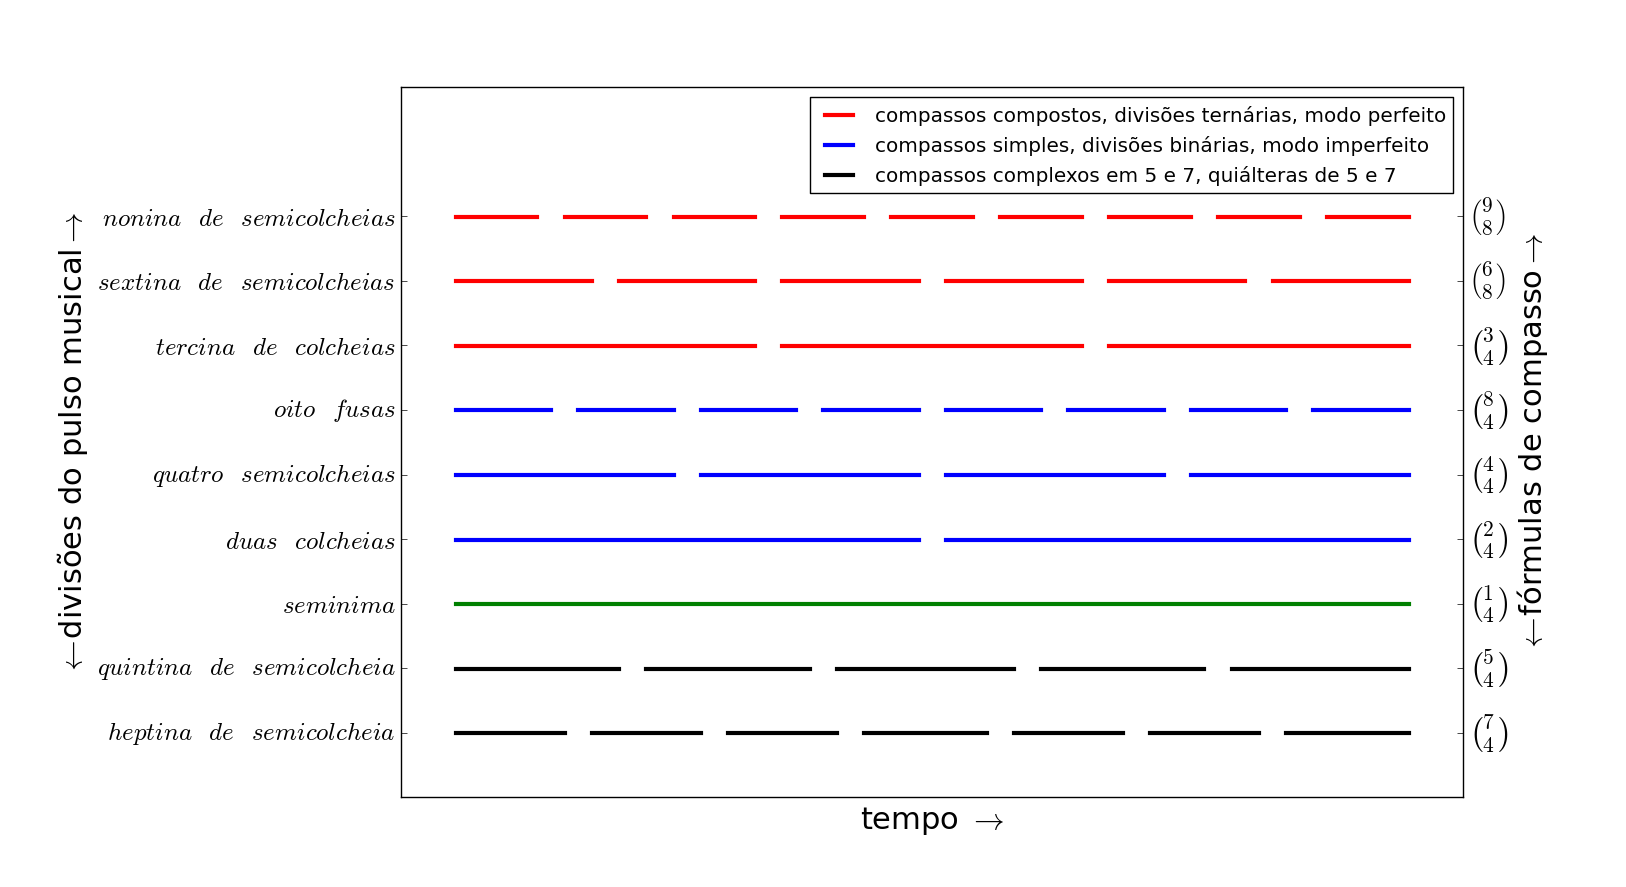
\includegraphics[width=\textwidth]{figuras/metricaMusical}
        \label{fig:pulsoSubAgl}
\end{figure}

As relações duais (compassos simples e divisões binárias) costumam a ocorrer em rítmos de dança
e ocasiões festivas e são chamadas imperfeitas. As relações triádicas ocorrem
incidem mais na música ritualística e relacionada ao sagrado
e são ditas perfeitas.

As divisões mais fortes (acentuadas) são as que consistem nas cabeças dos tempos. Nas divisões binárias (2, 4 e 8 dos casos considerados aqui),
as unidades consideradas fortes se revesam com as fracas
(e.g. a divisão em 4 resulta em forte, fraco, (meio) forte, fraco).
Nas divisões ternárias (3, 6 e 9 dos casos considerados neste escrito) a
à unidade forte (primeira) se sucedem 2 unidades fracas (e.g. a divisão em 3 resulta em forte, fraco fraco)\footnote{A divisão em 6 é considerada composta
 mas pode ocorrer também como uma divisão binária.
 Uma divisão binária que sofre então uma divisão ternária
 resulta em duas unidades divididas em três unidades cada: forte (subdividifo em forte fraco, fraco) e fraco (subdividido em forte, fraco, fraco).
A outra forma de ocorrer a divisão em 6 é através de 
uma divisão ternária que sofre então uma divisão binária, resultando em:
uma unidade forte (subdividido em forte e fraco) e duas unidades fracas (subdivididas em forte e fraco).}.

A acentuação em tempos fracos é chamada contratempo, as notas que se iniciam em tempos fracos e cuja duração percorre tempos fortes são as chamadas síncopas.

As notas podem ocorrer dentro e fora destas divisões (da \emph{'métrica musical'}). Nos casos mais comportados, as notas ocorrem exatamente nestas divisões, com maior incidência para ataques nos tempos fortes.

Com o fim de sistematizar e colocar em termos formais, podemos convencionar
o pulso como nível $j=0$ de agrupamento, o nível $j=-1$ 
é a primeira subdivisão do pulso, o nível $j=1$ como a primeira algomeração dos pulsos e assim por diante. 
Assim, seja $P_i^j$ a $i$-ésima unidade de 
pulsos no nível $j$ de agrupamento\footnote{Assim,
$P^0_{10}$ é o décimo pulso, $P^{1}_3$ é a terceira unidade de agrupamento de pulsos,
$P^{-1}_2$ é a segunda unidade da subdivisão do pulso.}.


Especial atenção para
os limites de $j$ pois as divisões do pulso devem resultar em durações apreciáveis
como rítmo e também as junções do pulso deve resultar algo apreciável como, no máximo
do nosso escopo, música. Dito de outra forma: a duração de $P^{min(j)}_i$, para $\forall \; i$
é maior que $50ms$ e as durações de $P^{\text{máx}(j)}_i$ \emph{somadas}  em $\forall i$
devem resultar em uma duração menor do que alguns minutos ou, no máximo poucas horas.


Para cada nível $j$ temos alguns índices $i$. Sempre que $i$ soma três 
(ou múltiplo de três) índices temos uma relação \emph{perfecta}, 
quando soma dois, quatro ou oito índices temos uma relação \emph{imperfecta}.


Podemos utilizar a notação

\begin{equation}
P^{ \{ j_k \} }_{\left \{ \{ i_{l} \}_0^{\alpha_{k}-1} \right \} } \quad \text{onde}\; \alpha_k \; \text{é o número de partições do nível} j_k
\end{equation}

para especificar qualquer unidade da subdivisão da métrica, com níveis $j_k$ e unidades $i_l$\footnote{Como um exemplo, podemos escrever $P^{-1,0,2}_{3,2,1}$  como a terceira subdivisão $P^{-1}_3$ do segundo
pulso $P^0_2$ do terceiro aglomerado $P^2_2$ de aglomerado de pulsos (perceba o termo $P^1_1$ omitido por simplicidade).}.

A cada unidade ou conjunto de unidades $P_i^j$ pode ser associada uma sequência de amostras temporais $T_i$
que formam uma nota musical. 

Usualmente lidamos com a distribuição rítmica dos eventos musicais com este arcabouço em mente. Assim como acontece com outras características
musicais, lidamos com a estrutura rítmica sem fórmulas pre-estabelecidas, deixando procedimentos sistemáticos para quando é pertinente.


\subsubsection{Estruturas direcionais}

Dadas as estruturas musicais básicas tanto frequenciais (acordes e escalas) quanto 
rítmicas (divisões e aglomerações simples, compostas e complexas) é 
natural pensar em como realizar estas estruturas de forma musical.

Neste ponto, encontramos alguns artifícios consagrados pelo tempo e pelo uso. 
Apresentamos aqui, de forma bastante breve, o pensamento musical dado por estruturas direcionais.
Na parte seguinte exploramos as estruturas recorrentes e cíclicas.

As estruturas direcionais nos possibiitam os recursos mais usuais: arcos melódicos e sequências que convergem ou divergem.

Os arcos melódicos são compostos por duas sequências convergentes: 
uma que atinge um ápice (chamado literalmente de clímax pela teoria musical canônica) e 
outra que, de forma paradigmática, volta do ápice à região da nota de partida.

Seja $S_i=\{s_i\}_0^{\Lambda_S-1}$ uma sequência crescente. A sequência 
$R_i=\{r_i\}_0^{2\Lambda_S -2}=\{s_{(\Lambda_S-1-|\Lambda_S-1-i|)}\}_0^{2\Lambda_S-2}$ 
é uma sequência perfeitamente simétrica\footnote{Apresenta simetria especular perfeita, i.e. a segunda metade é uma versão espelhada da primeira.}. Pensada segundo conceitos musicais, o clímax está exatamente no meio da sequência. 
Canonicamente, distinguimos também entre arcos cujos clímax estão deslocados do meio para o final 
e para o começo (e casos extremos disso, em que os climax estão no extato começo ou final)~\ref{schoenbergComp}.
Por razões ilustrativas, apresentamos no APÊNDICE XX alguns exemplos 
destas estruturas em casos da história da música.

\subsubsection{Estruturas cíclicas}
Os arcos musicais nem sempre são fruto de estruturas direcionais como as citadas
acima. Um caso crítico é o de estruturas que se modificam gradualmente
até atingirem o estado original, formando um arco cíclico.

Neste caso, faremos uma exposição específica sobre permutações dada
a solidez desta abordagem segundo princípios musicais, matemáticos e
filosóficos\footnote{De forma bastante resumida, apontamos o
entendimento filosófico de que o pensamento humano se baseia
em reconhecimentos de semelhanças e diferenças dentre os estímulos
e objetos~\ref{deleuze}. Portanto, segundo este entendimento,
as simetrias se encontram no cerne do processo cognitivo. Matematicamente,
as simetrias são representadas por grupos algébricos e os grupos finitos, por sua vez,
são sempre isomorfos a um grupo de permutações. Desta forma, podemos dizer que
as permutações são capazes de representar quaisquer simetrias em um sistema finito.
Diretamente na música encontramos permutações de forma bastante explícita, inclusive
na análise de música étnica~\ref{permMusic}.
Na tradição musical a permutação está presente em diversas técnicas~\ref{zamacois} e
apontamos em especial a técnica \emph{Change Ringing} que consiste essencialmente
em padrões de permutações dentre um fixado número de notas~\ref{change}.}.

Toda permutação pode ser operada com outra permutação, resultando na permutação
que representa a modificação de elementos fixados se aplicada uma permutação
depois a outra:

\begin{equation}
p_1 \bullet p_2 = p_3, \quad \forall \; p_1, p_2 \; \text{permutações finitas}
\end{equation}

Uma permutação finita aplicada sucessivamente um número suficiente de vezes
resulta na ordenação inicial dos elementos:

\begin{equation}
(p)^n = e \quad : \quad \text{se} \; p \; \text{finito} \; \Rightarrow \; \exists \;\; n  \in \mathbb{N} \; \text{e finito}
\end{equation}

O menor valor de $n$ é chamado de \emph{ordem} da permutação $p$. O elemento $e$ é chamado de elemento neutro e é
a permutação que leva uma ordenação para ela mesma.

A utilização de permutações na música pode ser resumida da seguinte forma:
seja $L_i$ uma lista de eventos musicais (para simplificar, considere
estes eventos musicais como sendo notas musicais) e $p$ uma permutação.
$L_i'=p(L_i)$ consiste nos mesmos elementos de $L_i$ com a ordem entre eles
modificada.

Importante notar que não é necessário permutar os elementos de $L_i$, mas somente
alguma ou algumas de suas características. Assim, seja $p^f$ uma permutação agindo
nas frequências e $L_i$ uma sequência de notas básicas como expostas
ao final de ~\ref{notaBasica}. A nova sequência $L_i'=p^f(L_i)$ consiste nas mesmas
notas musicais, na mesma ordem, com as frequências fundamentais permutadas segundo
o padrão que $p^f$ apresenta.

Por último, duas sutilezas deste procedimento.
Primeiro, a permutação $p$ não precisa envolver todos os elementos de $L_i$, i.e. ela
pode operar em subconjuntos de $L_i$. Segundo, nem todos os eventos $L_i$ precisam ser executados a
cada consulta de estado realizada.

Para simplificar, considere novamente os eventos de $L_i$ 
como notas musicais. Assim, se $i$ é vai de $0$ a $n>3$, a cada compasso
de $4$ notas podemos executar somente as primeiras $4$ notas. As outras notas de
$L_i$ podem ser incidentes nos compassos em que as permutações aloque
estas notas para as primeiras quatro notas de $L_i$.

Nada impede que tenhamos permutações operando no mesmo conjunto, cada uma destas permutações
$p_i$
possui: dimensões das notas em que opera (frequência, duração, fades, intensidade, etc),
modo de incidência (opera em $L_i$ a cada uma ou duas utilizações de $L_i$). Na realização das notas de $L_i$, uma solução fácil e coerente é executar as primeiras $n$ notas\footnote{A execução de notas disjuntas de $L_i$ equivale a modificar a permutação e executar as primeiras notas.}.

Esta abordagem resultou em alguns trabalhos ~\ref{figgusOriginal} e implementações computacionais. Descrevemos um uso coerente desta técnica abaixo e apresentamos no APÊNCIDE XX a implementação computacional disponibilizada em ~\ref{repoFiggus}


\subsubsection{Usos Musicais}
Algumas restrições funcionais possíveis: manter-se em harmonias triádicas e encadear os acordes
que possuam relações de quintas justas dentre as fundamentais ou dentre uma fundamental
e a terça do acorde seguinte.

Melodias e harmonias.

Explorações microtonais, oitava em 5 notas etc
FIGGUS














\clearpage


\section{Áudio e Música (deprecated)}

Por razões didáticas, dividimos este capítulo em 4 partes: música em tempo diferido (ou seja, que não é feito em tempo real),
música em tempo real,  música na matéria (suporte físico em hardware) e música no tecido social
(considerando especialmente as mobilizações humanas relacionadas).

Com isso desejamos expor a prática musical através do código
com exemplos reais de aplicação e em uso pelo autor, por membros do LabMacambira.sf.net,
por parceiros, colaboradores e por usuários eventuais das naturezas mais diversas.

  \subsection{Música em Tempo Diferido: Minimum-fi e FIGGUS}

\begin{quotation}
\small
'The increasing dominance of graphic interfaces for music software obscured 
the continuing presence of the command-line tradition, 
the code writer, the hacker. The code writing of deferred time 
computer programming may be assembled out of time order, debugged and optimized.'

\emph{Simon Emmerson, Living electronic music, 2007}
\end{quotation}

A realização musical em tempo diferido é o paradigma inicial da música computacional.
Iniciando com o Music V, a proposta foi depois desenvolvido com o CSound. Pode-se dizer
que até hoje é a forma como compositores usualmente pensam a música: pensando
e escrevendo as estruturas, que depois são executadas por instrumentistas ou aparelhos eletrônicos.

Assim como a composição instrumental permite um trabalho mais minucioso do que
a improvisação instrumental, a realização musical em tempo diferido usualmente permite um
detalhamento maior dos procedimentos do que a realização em tempo real. Por este
mesmo motivo, trataremos inicialmente de dois trabalhos em tempo diferido.
Aliás, como veremos a seguir, as abordagens completam uma base para a música
computacional praticada até os dias de hoje.

O som musical pode ser caracterizado físicamente, e sua síntese digital com base em nossa banda de audição e no teorema de Nyquist, sintetiza uma música amostra por amostra, através de princípios
claros de síntese sonora e organização musical\footnote{Veja no APÊNDICE XX: o \emph{minimum-fi} hi-fi, low-fi, minimum-fi, ou seja,
o mínimo de qualidade para assegurar existência e consistência
da criação}. O segundo, chamado de \emph{FIGGUS} (FInite
Groups in Granular and Unit Synthesis), utiliza os princípios do minimum-fi e constitui
um módulo Python completo, cuja proposta é a utilização de simetrias, através de
permutações e de Teoria de Grupos, para a composição de músicas. Como demonstração
das capacidades do FIGGUS, ele gera um EP\footnote{Extended Play, uma album musical maior que um single mas menor que um LP (Long Play) inteiro} com um único comando. Este é o
\emph{PPEPPS}\footnote{Pure Python EP: Projeto Solvente}, como veremos a seguir.

Desta forma, esta sessão exemplifica e explicita - através de dois exemplos reais - os
princípios do uso de código para a síntese \emph{musical}, desde as amostras
relativas a uma nota com dada frequencia, amplitude e timbre, até a confecção
de uma ferramenta derivada, já incorporando propostas musicais e estruturas
mais elaboradas.

      \subsubsection{Minimum-fi}

Existe uma perene matiz estética e também tecnológica
de realizar uma dada tarefa com \emph{o mínimo} necessário.
Esta matiz é para a música igualmente
fundamental e reconhecida como
princípio de unidade e coerência\footnote{Este princípio tanto é fundamental
que as escolas musicais possuem técnicas específicas, músicas possuem suas
próprias convenções mantidas por toda a sua duração, os arcos mantém características,
enfim, podemos até mesmo concluir que a simetria define o escopo.}. Em código computacional
a empreitada para manifestar este princípio ele próprio de forma mínima
resultou no \emph{minimum-fi.py}, código Python em um único arquivo curto que sintetiza
músicas com segundo as estruturas especificadas em linha\footnote{Em música se fala da \emph{bula} (que equivaleria
às funções em si e das especificações da linguagem) e a partitura ou 'música' propriamente ditas (que equivale à .}.
Na versão atual, de 2012 mas adiantada em 2011, os algorítmos 
em Python propriamente ditos somam 
53 linhas e inclui 5 funções. Com estas funções, estruturas musicais podem 
ser criadas padrão a padrão, nota a nota, amostra por amostra. Na prática e posto em
linguagem cotidiana, resultam em notas que formam
blocos e estruturas hierarquicamente superiores.


Os princípios, bastante simples\footnote{Osvaldo Lacerda, em seu livro \emph{Compendio de Teoria Elementar da Musica} fala das propriedades do som musical de forma equivalente.}, são:
\begin{itemize}
  \item Deve-se ter um mecanismo de síntese sonora que
possibilite a geração de unidades sonoras com diferentes timbres, controle sobre a frequência fundamental e duração específica\footnote{Também entra aqui o volume, mas como o que controlamos de fato é a intensidade relativa entre as notas, resolvemos por bem omitir
esta parte até que fiquem claros os códigos relativos a isso, logo abaixo.}.
  \item Deve-se ser capaz de construir não só unidades sonoras, mas também séries de unidades, sejam sobrepostas (acordes, por exemplo)
  ou justapostas (melodias, por exemplo).
\end{itemize}

Para o primeiro item, se prestam comumente os procedimentos de busca em tabelas/vetores com formas
de ondas em alta resolução (chamado \emph{lookup table}). O procedimento é barato e de qualidade alta
(não acrescentam ruídos relevantes ao sinal).

Para realizarmos a busca de forma eficiente, precisamos de tabelas que contenham cada uma
uma forma de onda. As tradicionais são a senoide e as ondas quadrada, triangular e dente de serra.
Mostramos a seguir estas formas de onda e também uma forma de onda retirada de um som real.

De posse destas formas de onda, A seguir está o procedimento da lookuptable:

\code{Procedimento de Lookup Table}{python_snippets/lookuptable.py}

O primeiro ponto importante é a tabela em si, usualmente unidimensional. É de comum conhecimento que
tabelas com 1024 são mais que suficientes para os usos musicais e a diferença
de qualidade (relação sinal/ruido) não muda consideravelmente com a utilização
de tabelas maiores. A seguir dispomos algumas destas tabelas, mais 
especificamente, dispomos as tabelas para os formatos de onda mais usuais. 

\code{Formas de Onda Tradicionais}{python_snippets/formasDeOnda.py}

Através da utilização do lookup sucessivo (procura-se um valor na primeira tabela
e este valor indica o valor na segunda tabela a ser utilizado), executamos
um waveshaping. Este procedimento é bastante apreciado pela simplicidade e eficácia
na síntese de tímbres diversos e ricos em harmônicos e evolução temporal. Embora
uma explicação exaustiva do waveshaping fuja ao escopo deste trabalho, este
método se caracteriza pela aplicação de uma função não linear ao sinal de entrada.
Neste caso o sinal de entrada é gerado pelo primeiro lookup, a função não linear aplicada
é representada pela segunda tabela e aplicada pelo segundo lookup.

Existem muitas formas de se executar waveshaping, a seguir segue o que usamos no minimum-fi, que se sustenta principalmente por ser leve e simples:

\code{Waveshaping com Lookups sucessivas}{python_snippets/lookup_cruz.py}

O segundo item - dos dois princípios expostos sobre o minimum-fi - presta-se à discretização do espaço musical. Unidades como batidas e notas
tornam mais eficiente a comunicação pois a quantidade
de estruturas sugeridas é maior e as estruturas são mais claras no discreto do que no contínuo~\cite{Roederer}. Roederer chega a
apontar que as próprias notas dos instrumentos musicais são um reflexo de que é mais eficiente
o uso do discreto do que do contínuo para a geração de estruturas musicais.

De fato, unidades bem definidas se mostram úteis na prática musical 
para fazer sequências de unidades, concatená-las. Quando as unidades
são notas, as sequências de unidades justapostas no tempo são melodias ou linhas melódicas. As
sequências sobrepostas no tempo são comumente pensadas como acordes, mas podem ser tidas simplesmente
como sobreposições circunstanciais de duas linhas melódicas. Isso, claro, segundo
a sistematização clássica e usual da música~\cite{Lacerda}\footnote{Vole assinalar aqui que a música do século XX apresentou diversos modelos teóricos que quebram com este entendimento simplificado sobre a música, suas unidades básicas e estruturas relacionadas}.

As duas construções básicas explicitadas a seguir, baseadas na dicotomia melodia/harmonia
(horizontalidade/verticalidade, justaposição/sobreposição), são
as funções \emph{fazSequencia} e \emph{fazAcorde} no minimum-fi. Vale notar elas são absolutamente 
equivalentes em uma análise puramente conceitual, i.e. uma delas pode ser omitida segundo algumas teorizações. Isso fica particularmente óbvio quando se nota que os procedimentos de mixagem e concatenação são
plenamente capazes de realizar o que estas funções realizam. Aliás, as funções nada
mais são do que usos típicos e quase caricatos destes procedimentos: no fazAcorde a mixagem
sobrepõe no tempo todas as unidades, no fazSequencia as unidades são todas juntapostas no tempo.

Como pode-se notar a seguir, as sequências de notas e os acordes, em última instância, são utilizações específicas das 2 funções de síntese sonora explicadas anteriormente: lookup e lookupcruz.

\code{Realização de Sequências de Notas}{python_snippets/fazSequencia.py}

\code{Realização de Acordes de Notas}{python_snippets/fazAcorde.py}

A última das cinco funções utilizadas é uma soma amostra a amostra de dois sons. Para isso,
é necessário completar com zeros a sequência com o menor número de amostras para somar rapidamente:

\code{Somador (função auxiliar)}{python_snippets/somador.py}

Depois disso é usufruir com estruturas criadas. Por exemplo: depois de construidas
algumas tabelas para serem usadas como diferentes timbres, pode-se criar as
escalas completamente simétricas na oitava cromática assim:

\code{Escalas Completamente Simétricas (na grade dos 12 semitons e no âmbito da oitava)}{python_snippets/escalas_simetricas.py}

% escala\_1=range(12) # cromática ascendente sem inclusão da oitava
% escala\_2=range(0,12,2) # tons inteiros
% escala\_3=range(0,12,3) # diminutão
% escala\_4=range(0,12,4) # terças maiores
% escala\_6=range(0,12,6) # trítonos
% \end{python}
% \input{py}

Sendo cada unidade um semitom. Ou seja, cada unidade é o fator que fica presente na conta $f_0 . 2^{(1/12)} . fator $ e resulta na frequência exata da nota relativa a $f_0$ em um sistema temperado ideal.

Podemos também utilizar as usuais
escalas tonais maior e menor natural, harmônica e melódica:

\code{Escalas diatônicas tonais (maiores e menores)}{python_snippets/escalas_Mm.py}

A utilização de intervalos menores que o semitom\footnote{Prática também conhecida
como \emph{microtonalismo}, que gera/utiliza \emph{microtonalidade}.} mostra-se trivial em
nossa implementação. Basta representar sequências de fracionários
que são partes linearmente proporcionais dos semitons ou modificar o fator $f$:

\code{Escalas Microtonais (com quartos e oitavos de tom e intervalos menores)}{python_snippets/escalas_microtonais.py}

Da mesma forma, as triades maiores e menores
são especificadas com simplicidade. Note que aos acordes \emph{diminutão} e
\emph{aumentado} correspodem as mesmas notas das escalas simétricas de terças menores
e maiores respectivamente:

\code{Acordes anotados como listas em python}{python_snippets/acordes.py}


E séries/sequências podem ser anotadas junto a variações:

\code{Séries diversas}{python_snippets/series.py}

Com este arcabouço, o passo seguinte é sintetizar e mixar, resultando
em sequências musicais. A síntese de sequências e acordes são feitos tipicamente
através de comandos desta forma:

\code{Sintetizando sequências e acordes}{python_snippets/seqs_acordes.py}

Já a síntese de estruturas compostas (p.ex. sequências de acordes e sobreposição
de linhas melódicas), são feitas com os recursos usuais da liguagem. Neste caso
usamos listas em Python e implementações em Numpy (mais eficientes em tempo de
execussão e também na simplicidade do código) estão no apêndice. Estes mesmos
procedimentos são praticamente os mesmos em Scilab, C/C++, Javascript, PHP, etc.

A seguir demonstramos para fins didáticos, a construção de acordes periódicos em
python puro\footnote{A implementação não didática destas três linhas de código
podem ser agrupadas em uma só linha.}:

\code{Acordes periódicos}{python_snippets/acordes_periodicos.py}

Em posse destas sequências, acordes e recursos da linguagem,
formamos estruturas hierarquicamente superiores
através da concatenação de estruturas, da mixagem de estruturas, e da amplificação
(ou atenuação) seletiva das mesmas:

\code{Amplificação e mixagem}{python_snippets/amp_mix.py}

Neste ponto, basta criarmos músicas e sequências de interesse estético ou para pesquisa. Dado o ferramental, os encadeamentos dependem de intensões estéticas, entendimentos musicais e estruturas abstratas que mantém a coerência e interesse em uma peça musical. Para o leitor mais interessado, deixamos para o Apêndice X um exemplo de música feita com o minimum-fi. A seguir utilizamos esta base apresentada para sintetizar estruturas musicais e então um EP.

\vspace{10 mm}

        \subsubsection{FIGGUS: FInite Groups in Granular and Unit Synthesis}

Em coerência com os conhecimentos
e tecnologias já apresentados nesta exposição\footnote{Especificamos o arcabouço para geração de sons musicais em unidades
e estruturas compostas logo acima na subsessão sobre o minimum-fi.}, introduzimos agora
um foco especial nas estruturas musicais
desenvolvidas. São elas, inseridas em um momento histórico e
executadas por instrumentos específicos com as técnicas de época,
que constituem uma linguagem musical e músicas propriamente
ditas[ref]. O FIGGUS constitui uma técnica composicional
manifestada em software como ferramenta de síntese de
estruturas musicais por estruturas matemáticas específicas
para representação de simetrias.

Este desenvolvimento foi iniciado em 2006 com o físico-matemático Prof. Adolfo Maia Junior - bem anterior
ao nascimento do minimum-fi - para
tratar de simetrias na música com vistas à composição musical através
de métodos matemáticos\footnote{Duas iniciações científicas trataram do assunto, convenios XXX e YYYY.}. Mais especificamente, a proposta resultou em
um programa voltado para a síntese
granular e síntese de estruturas musicais através de Grupos Algébricos. O nome dado
foi FIGGUS, sigla de FInite Groups in Granular and Unit Synthesis\footnote{Também utilizamos
o nome FIGGS (FInite Group in Granular Synthesis) dado que o termo \emph{unit synthesis} não
é usual na literatura. Posteriormente o primeiro autor deste trabalho recorreu novamente
ao uso do nome FIGGUS. Isso foi motivado principalmente pelo fato de que
o maior uso da técnica é para síntese de estruturas musicais, não para
síntese de amálgamas sonoros (ou timbres mesmo) tipicamente resultantes da síntese granular}.

Na atual reescrita, embora ainda bastante atrás do FIGGUS original quanto
à interface gráfica, a ferramenta opera diretamente em Python puro,
com as biblitecas imbutidas por padrão. Isso permite com que o FIGGUS
sintetize todo um EP usando somente os comandos:

\code{Utilizando o FIGGUS para Sintetizar um EP}{python_snippets/synth_ep.py}

Desta forma, a ferramenta fica muito mais simples para experimentações
e implementações adicionais pois sua utilização se dá através
do próprio código no qual tudo é especificado. Esta abordagem se mostra particularmente
pertinente pois a estagnação do mecanismo de síntese de estruturas musicais
beira a inviabilização do uso artístico ou torna necessário o uso
de recursos externos.
Outro uso pretendido para o FIGGUS
é a síntese de tímbres e amálgamas sonoros através da
Síntese Granular. Embora nosso foco seja outro, cabe algumas breves
palavras sobre o assunto.

A Síntese Granular é uma área bem estabelecida tanto na acústica quanto
na Computação Musical e se caracteriza pela geração de sons bastante curtos
e em quantidade massiva. Tipicamente os sons possuem entre 5 e 40 milissegundos
e a quantidade destes \emph{microsons}\footnote{Grãos sonoros e microsons são jargões
típicos da síntese granular usados para indicar sons com as durações especificadas
no texto.} pode chegar a milhares por segundo. O tratamento específico da
síntese granular foge ao escopo deste trabalho e indicamos ao leitor interessado
os artigos produzidos sobre Síntese Granular e Teoria de Grupos[refs AES e SBCM].
Assim, focamos o texto a seguir em Grupos Finitos e Síntese de Estruturas Musicais.

Nas artes é de comum conhecimento o papel absolutamente central
que as simetrias possuem. Na música, para citar somente alguns exemplos simples,
temos os numerosos estudos de simetrias na música de J. S. Bach, os jogos
de dados de Mozart e os usos recorrentes da proporção áurea na música
de Béla Bártok. Matematicamente, as \emph{simetrias} são descritas por Grupos,
e estes são definidos como sendo um conjunto (chamemos de $G$)
munido de uma operação (seja $\bullet$), formando um grupo $(G,\bullet)$
satisfazendo as seguintes propriedades:

\begin{enumerate}
    \item Fechamento: $\forall \ g_1, g_2  \in G \Rightarrow g_1 \bullet g_2 \in G$
    \item Associatividade: $(g_1 \bullet g_2) \bullet g_3 = g_1 \bullet (g_2 \bullet g_3), \forall \ g_1, g_2, g_3 \in G$
    \item Existência do elemento neutro: $\exists \ e \in G : g \bullet e = e \bullet g = g$
    \item Existência dos inversos: $\forall \ g \in G \ \exists \ g^{-1} : g \bullet g^{-1} = g^{-1} \bullet g = e$
\end{enumerate}

Adicionalmente, vale complementar que se um grupo tiver um número
finito de elementos, ele é dito finito, caso contrário é chamado
infinito. Todos os elementos de um grupo finito são cíclicos pois
operado com si próprio um número suficiente de vezes resulta em si
mesmo. Um grupo é dito comutativo ou abeliano caso a propriedade
comutativa seja satisfeita para todos os elementos:
$\forall \ g_1, g_2 \in G \Rightarrow g_1 \bullet g_2 = g_2 \bullet g_1$.

São numerosas as aplicações de grupos e estes
usos para as artes possam se desenvolver
de diversas formas focadas em simetrias
e com interesse estético, em
nossas pesquisas uma delas se mostrou particularmente coerente
e pertinente: as permutações de unidades sonoras. Primeiro,
através do Teorema de Cayley, todo grupo finito é isomorfo
a um grupo de permutação\footnote{Mais especificamente,
todo grupo é isomorfo a um subgrupo do grupo simétrico agindo
em G.}, i.e. seus elementos são diretamente relacionados
a permutações. Além disso, na música as permutações estão
no núcleo de diversos procedimentos canônicos como a
retrogradação e outras técnicas de variação.

[Expor sobre uma ou duas músicas feitas com o FIGGUS]

No FIGGUS, implementamos o grão sonoro (no caso mais usado
como unidade) como uma classe que possui apenas
os seguintes atributos (e não possui funcões): duração (segundos),
frequência (Hz), timbre (identificador para usar mediante implementações convenientes), intensidade (pico $\in \ [0,1]$), e duração dos fades (in e out em segundos). Aqui a classe:


\code{Grão Sonoro Básico}{python_snippets/fgrao.py}

O FIGGUS funciona com base em uma sequência de grãos posta de antemão
na qual operam as permutações. Além da sequência de grãos,
é conveniente também manter o número de grãos da sequência e uma
lista com os índices dos grãos para executar as operações necessárias para gerarmos as músicas (ver abaixo). A classe utilizada para representar as sequências é assim:

\code{Sequência de Grãos}{python_snippets/fsequencia.py}

Aos grãos em sequência neste ponto são aplicadas permutações.
Para isso é bastante conveniente representar as permutações em classesseparadas e os padrões de aplicação destas permutações para facilitar
desenvolvimentos com clareza. No caso a classe de permutações só possui os parâmetros da permutação em si e do tamando dela (número de elementos que ela utiliza). É conveniente implementar uma tradução da notação cíclica para a notação direta da permutação e é uma das facilidades da implementação por classe que fizemos. A classe do padrão de permutação possui também um período de aplicação da permutação, ou seja, de quantas em quantas leituras da sequência aplicamos a permutação. As classes ficaram assim:

\code{Permutações e Padrões de Permutações}{python_snippets/fpermutacoes.py}

De posse dos grãos, da sequência, das permutações e do padrão de permutações estamos possibilitados de realizar a estrutura musical em si. Bastam adicionalmente, especificar o número desejado de iterações da sequência. Com isso, a sequência de grãos é lida um número de vezes, aplicando as permutações na sequência segundo o padrão de aplicação das pemutações, de forma a resultar em uma sequência sonora musical. Note que se a permutação usar menos elementos que a sequência possui, alguns destes elementos ficarão estáticos nas iterações da sequência no padrão sonoro.

Na síntese do vetor sonoro relacionado, é também crucial estabelecer a taxa de amostragem preterida, como podemos perceber na função de síntese dos vetores, da classe Pattern que cuida desta realização do padrão em si. Deixamos a seguir esta função, de forma que faltará apenas a escrita destes vetores sonoros em arquivo de áudio, como veremos a seguir.

\code{Realização do Padrão Musical}{python_snippets/fpadraosonoro.py}

Em posse não apenas de representações abstratas do padrão musical a ser realizado, mas dos próprios vetores sonoros relacionados à representação digital da música a ser realizada, podemos escrever este vetor como um arquivo de áudio propriamente dito. O mais conveniente neste caso é escrever um arquivo PCM (Pulse Code Modulation) em padrão amplamente utilizado e reconhecido. Ambos os padrões WAV e AIFF satisfazem estes requisitos e escolhemos o WAV por ser o padrão de CDs (Compact Discs) e também o mais utilizado por programas de áudio. Mais especificamente, o padrão de CDs é WAV com 44100 amostras por segundo e 16 bits por amostra\footnote{No formato WAV de CD, cada amostra é representada por uma variável inteira 'signed' de 16 bits.}. As amostras dos vetores sonoros são calculados, por conveniência e por convenção, no âmbito $[-1,1]$ e precisam ser normalizados para o âmbito $[-32767,32768]$ e truncados em números inteiros. Depois disso precisam ser escritos em um arquivo com os bits como na convenção da linguagem C/C++. A bibioteca \emph{struct} cuida dessa escrita do inteiro no formato correto, e a biblioteca \emph{wave} escreve o cabeçalho no formato WAV adequado. Assim, a clase de escrita do vetor sonoro em arquivo comum fica assim:

\code{Escrita do Vetor Sonoro em Arquivo WAV}{python_snippets/fio.py}


  \subsection{Música em Tempo Real: Livecoding e ABeatTracker (ABT)}

Com os avanços computacionais recentes, tornou-se usual a síntese sonora
em tempo real. Com isso, surgiram liguagens dedicadas para o áudio e a música
em sua maioria dedicadas - ou ao menos capacitadas - para o uso 
em tempo de execussão [citar PD, SC, ChucK]. Em outras palavras, estas linguagens
possibilitam que o usuário ouça o resultante sonoro do código utilizado e altere
o código com resultado imediato no processamento e resultado que escuta.

Nesta linha de exploração musical do código, iremos expor a seguir sobre
nossas investidas em \emph{Livecoding} (escrita de código em tempo real
com vistas à performance pública) e o ABeatTracker (uma linguagem por macros
para execussão sonora rítmica em conjunto com instrumentos tradicionais e outras
fontes sonoras/musicais externas).


        \subsubsection{Livecoding}

Recentemente, grupos de ponta em música experimental no mundo todo estão
desenvolvendo apresentações musicais públicas baseadas na escrita
de código ao vivo. Usualmente, se projeta o código para que a audiência possa
ver o que está sendo escrito, no rítmo em que se escreve, e se projeta também
o resultante sonoro por autofalantes.

As motivações para isso são variadas. Expomos a seguir de forma topificada
um condensado do que nos orientou a tal prática. Vale ressaltar que são
motivações igualmente presentes em outros grupos, embora não necessariamente
em todos ou da mesmícima forma.

\begin{itemize}
    \item A performance musical por computador carece de recursos performáticos
    à altura das execussões com instrumentos tradicionais. Os gestos são por demais
    discretos e a concentração do performer é bastante focada na tela do computador.
    \item O feedback auditivo do código projetado permite que o espectador infira
    significados dos códigos. Mesmo que de forma superficial, este recurso do livecoding
    é em muito capaz de desmistificar a programação de computadores, por muito considerada
    completamente intangível.;
    \item O código em si é um recurso poderosíssimo, que permite ao usuário controlar
    os sons produzidos amostra por amostra ou em escalas maiores, como notas, compassos, fraseados
    inteiros ou mesmo em escalas maiores de tempo, como minutos, horas, dias e semanas.
    \item O compartilhamento do código é usual, leve e eficiente como entrega completamente
    aberta da tecnologia relacionada à proposta estética.
\end{itemize}

Desta forma, iniciamos em 2011 uma linha de atuação com Livecoding que resultou em uma performance
no \emph{V Festival Contato}. Utilizamos a linguagem ChucK por apresentar os recursos que
consideramos mais apropriados, embora de forma alguma isso seja consensual na prática atual
de livecoding.

A apresentação contou com recursos adicionais para agregar interesse, como a utilização
do \emph{cowsay} (para enviar mensagens enquanto se desenrolava a música) e trajetórias
de um ponto no fundo do código para sugerir a vertigem do sono REM. Estes recursos
podem ser vistos em uso claramente nos videos demonstrativos [citar videos do vimeo].
As linhas do cowsay e o script em processing relacionados estão no Apêndice XX...

Duas pessoas executaram livecoding simultaneamente. A saber, Vilson Vieira executava
rítmos, batidas bastante marcadas que serviam como base. Renato Fabbri, autor do presente
trabalho, executava linhas fluídas quasi melódicas que formavam arcos maiores. Nos intervalos
das investidas no formato citado, havia interlúdios em que ambos se revesavam com músicas
curtas e inusitadas, como em um duelo[disponibilizar músicas em links e colocar de referencia].

[Colocar os códigos meus e do Vilson e explicar o funcionamento e uso]





      \subsubsection{ABeatTracker (ABT)}
O ABT é uma linguagem/ferramenta que dispara linhas rítmicas através de macros que especificam
as células rítmicas, amostras sonoras que são utilizadas como conteúdo sonoro destas
linhas, modos de leitura destas amostras sonoras, e variáveis randômicas utilizadas
para execussão da linha. Além disso, o ABT dispõe de variáveis globais que podem ser alteradas
a qualquer momento pelo usuário, como BPM, velocidade de leitura das amostras e variáveis
randômicas globais (que se somam às individuais).

Em pouco explicitaremos a forma de utilização do ABT. De antemão, é pertinente apresentar
uma pequena discussão a respeito do que o ABT é considerado e sobre os propósitos desta
ferramenta. Em primeiro lugar, vale manter em mente que o ABT tem um funcionamento específico
que pode transcender o que se conhece por livecoding. As macros pré-estabelecidas engendram um
conjunto de recursos pré-estabelecidos bem definido, o que contrasta com a ideia de uma 'linguagem
de programação' que tenha capacidades mais amplas. De qualquer forma, linguagens com domínios
específicos não são raras e por vezes o ABT foi descrito como uma linguagem.

Sobre os propósitos do ABT, em primeiro lugar ele se dispõe a ser um instrumento computacional
essencialmente rítmico. Junto a esta proposta, vem a necessidade da utilização em conjunto com
outros instrumentos, externos ao ABT, ao computador em que estiver rodando e possivelmente externo
com relação a qualquer computador. Para isso foi elaborado o ABD (ABeatDetector), no qual o usuário
tamborila os rítmos que estiver ouvindo ou imaginando para que o ABT sincronize o pulso e utilize
células rítmicas relacionadas. A análise feita pelo ABD resulta em uma série de rítmos explicitados
por sequências de compassos que encapsulem durações regulares do rítmo tamborilado. Estes rítmos
relacionados ao tamborilar do usuário são chamados de harmônicos e podem ser selecionados
prontamente para o disparo de linhas melódicas.

No Apêndice XX está o manual de utilização do ABT e todo o código do ABT (e do ABD) está
disponivel online (citar repos). Exploramos abaixo detalhes relevantes da implementação,
em especial a forma de funcionamento do ABD.

[códigos-chave e explicações sobre o ABT e o ABD]




  \subsection{Música na Matéria: EKP e AHT}

Embora o foco deste trabalho seja na exploração musical através de códigos (abertos!),
nesta sessão iniciamos uma explicação simples, clara e factual de como estas
investidas transcendem o código e até mesmo a música em si.

Mais relevantes que os desenvolvimentos em si, são as mobilizações criadas nos
entornos e os engajamentos. Isso ficará evidente nas próximas - curtas - sessões
destes desenvolvimentos e resultados.

Aqui apresentamos dois trabalhos que geraram alguma movimentação de pessoas,
resultando em reuniões, desenvolvimentos, pesquisas e apresentações propriamente
ditas. O primeiro utiliza o estado do hardware como entrada, o segundo se trata
de uma mesa escultural para flutuação de origamis que resulta em um instrumento musical
bastante lúdico.


      \subsubsection{Emotional Kernel Panic (EKP)}

Em 2008, colaborando intensamente com o CDTL
(Centro de Desenvolvimento de Tecnologias Livres)\footnote{foi uma associação civil formada e desmembrada em 2008 e sediada em Recife, PE}
foi lançada a ideia de utilizar o estado do sistema operacional - especialmente o kernel linux - para
geração de sons. Surge o Emotional Kernel Panic (EKP) na colaboração excepcional de
Felipe Machado\footnote{Importantíssimo para o desenvolvimento da Cultura Digital no Brasil [citar fontes e programas governamentais]},
Ricardo Brazileiro\footnote{Artivista Digital bastante ativo [citar fontes]} e o primeiro autor do presente trabalho.

Desde o inicio, foram definidos três finalidades
para esta exploração do SO:

[visitar o README do EKP e achar os scripts do Brazileiro sobre o EKP]

\begin{itemize}
    \item Didáticos
    \item Artísticos
    \item Monitoramento do SO
\end{itemize}

Toda a base do EKP está aqui: http://trac.assembla.com/audioexperiments/browser/ekp-base

[Patches desenvolvidos por Brazileiro/Machado e rascunho do EKP-Monitor]

      \subsubsection{AirHackTable}

A AirHackTable é um instrumento musical eletrônico controlado por origamis (dobraduras de papel), construída na forma de uma mesa. Nela, uma rede de coolers reciclados faz flutuar origamis de geometria e cores variadas. Os movimentos dos origamis são captados por webcam e interpretados em tempo real por software de processamento de imagens, gerando padrões que controlam a transformação sonora da música. Dessa forma, pode-se dizer que os sons gerados refletem o voo dos origamis de acordo com suas geometrias (que geram trajetórias de voo caracteristicas).

Na versão atual da AirHacktable, cada cor (vermelho, amarelo, azul, verde, preto, ou branco) controla uma voz, e a posição do origami na mesa modula aspectos do som. Em outras palavras, se o origami está flutuando mais à esquerda, o som sai no canal à esquerda da mesa, e se o origami está mais próximo da câmera, o volume aumenta, e se está mais afastado do operador, o som se torna mais agudo. 

[imagens da AHT e dos patches em operação]

   \subsection{Música no Tecido Social: Sabrina Kawahara, Audioexperiments, EstudioLivre.org, CDTL, juntaDados.org, Devolts.org, MSST, LabMacambira.sf.net}

Esta é uma sessão menor, dedicada a apontar repercussões emergentes destas empreitadas em comunidades diferentes
e então tornar compreensível o desdobramento que estes códigos dedicados à música tiveram em processos sociais
e mobilizações civis.

Grupos foram montados em torno destes desenvolvimentos. Como os propósitos de compartilhamento
e apropriação tecnológica estavam no cerne dos grupos relacionados, as investidas
naturalmente tomaram teores engajados socialmente. A questão do empoderamento das pontas
e da criação de um patrimônio tecnológico da humanidade é consequência quase imediata
das posturas de compartilhamento e apropriação citados.

Discorremos brevemente sobre cada uma das iniciativas citadas:

\begin{itemize}
    \item Sabrina Kawahara
    \item Audioexperiments
    \item Estudiolivre.org
    \item CDTL
    \item JuntaDados.org
    \item Devolts.org
    \item MSST
    \item LabMacambira.sf.net
    \item Outros relacionados: MuSa, Metareciclagem, Submidialogia, Tainã
\end{itemize}


\section{Web}

  Difusão de informação com ênfase na facilitação
  da apropriação de tecnologias e de instancias políticas.

   \subsection{Tecnologias sociais de alta demanda: Sitios, Conteúdos e Articulação}

      \subsubsection{Sítios}

      FDDCA

      Ferramenta de comunicação

      (Cadastro dos pontos?)

      AA, SOS, Catalogo de Ideias, etc

      Meu site pessoal


      \subsubsection{Conteúdos}

      Wiki?

      \subsubsection{Articulação}

      IRC, Emails

\subsection{Disponibilização e desenvolvimento conjunto: wikis, etherpads, AA, Trac, IRC ..}

\subsubsection{Wiki}

\subsubsection{Trac}

\subsubsection{Screencasts - Vimeo}

\subsubsection{AA}

\subsubsection{Audio Experiments (Æ)}

\subsubsection{IRC}

\subsubsection{Etherpads}

\subsubsection{Outras fontes}


\section{Materiais didáticos}

  \subsection{Tutoriais em texto e código: Filtros, Nyquist e plugins LADSPA}

Os vários materiais didáticos produzidos constam no apêndice
deste trabalho. Um único destes será exposto a seguir por sua
capacidade de agregar os conteúdos dos capítulos anterioes:
os tutoriais de filtros e amostragem.

\begin{itemize}
    \item {\bf Tutorial de python para áudio e som}

Este tutorial foi levado para Berlim no LAC 2007 e sofreu melhoras desde entao. Esta
primeira versao ficou resumida em forma de texto no EL\footnote{http://estudiolivre.org/python-e-som-tutorial}. Em 2010
a Associacao Python Brasil escolheu este trabalho, então já mais amadurecido, para ser apresentado no
FISL em Porto Alegre. Como consequencia, foi feita uma série de video-tutoriais bastante utilizados\footnote{http://estudiolivre.org/tiki-index.php?page=Video+Tutoriais}.
Este tutorial foi comentado em listas em que o autor não participa (e outras em que o autor participa).

    \item {\bf Tutoriais de filtros e amostragem via python}

Voltados para explicitar principios fundamentais de áudio, estes tutoriais
são baseados código Python e o equivalente em C. Pequenas explicações são
dadas com o intuito de orientar a exploração inteligente destes \emph{snippets}.

\emph{Teorema de Amostragem}: estes scripts visam a experimentacao inteligente com
o Teorema de Nyquist. (descricao)

\emph{Filtros}: alem da explicitação sobre as diferenças entre filtros FIR e IIR,
duas utilizações clássicas destes filtros estão implementadas: Wavelets (FIR) e Quad (IIR)

Estes códigos podem ser baixados no repositório SVN do AudioExperiments. E os textos estão
na wiki (nos digitais ou EL, recriar pois os CDTL foram apagados)

    \item {\bf Tutorial de plugins lv2}

Dadas as dificuldades que o desenvolvimento dos \emph{plugins} de áudio apresenta,
desenvolvi um tutorial passo a passo com plugins que rodam em todas as etapas.
Ele é baseado em uma interface C++ para este padrão de plugin que eh implementado
em C. Os códigos e os textos estão todos em repositório.

    \item {\bf Microtutoriais Django ~\cite{dmicrotuts}}

Estes 'microtutoriais' são baseados nos conceitos de \emph{scripts mínimos} e
\emph{alterações puntuais}. O primeiro conjunto de microtutoriais é dedicado
a reconstruir o tutorial oficial do django de forma condensada e não prolixa.
O segundo destes conjuntos é dedicado a instrumentalizar de fato o leitor com
o entendimento do funcionamento dos princípios fundamentais deste framework.

    \item {\bf Philosometrics}

Embora este não seja um trabalho didático propriamente dito, ele tem este intuito
no cerne de sua concepção e surgimento. Em decorrência dele, surgiu o  Musimetrics,
o Cinemetrics e o Literametrics. Além disso, ele é um belo exemplo da
utilização das ciências duras para a análise de ciências humanas e foi acolhido
como tal em alguns momentos.

    \item {\bf Carta mídias livres}

Texto criado em decorrência da participação da comissão de seleção no
'Prêmio Mídias Livres', a convite do Ministério da Cultura por 'notório saber'.
Esta carta é um documento único no seu conteúdo, deixando às claras
o conceito de Mídias Livres como mídias não aprisionadas pelo conceito
de propriedade, ou seja, que priorizam a sua livre circulação e a possibilidade
de geração de materiais derivados, assim como sua geração aberta ao colaborativo e comunitário.

    \item {\bf Textos de cunho sociológico, transformador}

Produção mais numerosa que as anteriores, se caracteriza por métodos não convencionais
de abordagem dos assuntos e de escrita. Em especial utiliza-se pseudônimos para
auxiliar a despersonificação, gerando textos menos presos à satisfação da auto-imagem, dente
outras qualidades. A utiliação de psudônimos é um costume muito apreciado em diversos meios,
e as pesquisas tem confirmado as vantagens que a prática apresenta e confirma\footnote{http://disqus.com/research/pseudonyms/}.

O autor destes textos se dá ao direito de não revelar seus psudônimos - embora muitos deles
sejam publicamente conhecidos - para conservar as consequências desta prática na
forma mais pura. Como comprovante desta produção, deixamos uma mensagem sobre a publicação
de textos em mídia impressa com autores internacionais,
confirmando a participação do autor desta dissertação, mas cujo
nome não consta na publicação.

!!!!!!!!!!!!!!!!!!!!!!!!!!!!!!!!!!!!!!!

de      fabi borges catadores@gmail.com por  riseup.net 
responder a     submidialogia@lists.riseup.net
para    submidialogia@lists.riseup.net
data    23 de agosto de 2011 12:26
assunto Re: [submidialogia] livro sub- publicação
lista de e-mails        <submidialogia.lists.riseup.net> Filtrar as mensagens dessa lista de e-mails
enviado por     lists.riseup.net
assinado por    riseup.net
cancelar inscrição      Cancelar a inscrição para essa lista de e-mails
        Importante principalmente porque você frequentemente lê mensagens com esse marcador.
ocultar detalhes 12:26 (6 minutos atrás)
entao, eu fui recebendo textos durante esse tempo,
alguns tao atrazados como dos sem satelites, mas muita gente mandou;

aqui os autores:

os internacionais nao sao muitos, o joni kempf (o que bebe ouro do hardware), o barbrook (futuros imaginarios),
Hamdy heda (da revolucao egipcia), o pedro soller (summerlab), maria llopis (pos porno),  talvez a bronac, nao entregou ainda.

dos brasileiros, renato fabri, ruiz, pasteur, morgana e caio, ju dornelles, mari marcassa, coletivo errorista, adriana velozo-drica, tiago pimentel, felipe fonseca, thiago novaes, lelex, felipe ribeiro(?), maira, verenilde,  bartolina silva, poro, vitoria amaro, fabib (eu),

entao, precisa publicar agora,
uma equipe para publicacao e,,, 

bjs
f

!!!!!!!!!!!!!!!!!!!!!!!!!!!!!!!!!!!!!!!

\end{itemize}

\subsection{Screencasts e outros materiais em video e em texto}

\begin{itemize}
    \item Python para áudio e música
	  Texto - palestras - videos

    \item Canal Macambira
No Macambira estão sendo produzidos materiais em screencasts sobre
diversas cenas de hackeamento.

    \begin{itemize}
	\item Live-Coding
	\item Raspagem de dados
    \end{itemize}
\end{itemize}
